\documentclass[10pt,letterpaper]{article}

% ===============================
% PACKAGES
% ===============================
\usepackage{geometry}
\usepackage{setspace}
\usepackage{fancyhdr}
\usepackage{tcolorbox}
\tcbuselibrary{skins, breakable}
\usepackage{titlesec}
\usepackage{tocloft}
\usepackage{hyperref}
\usepackage[numbers,sort&compress]{natbib}
\usepackage{url}
\usepackage[table]{xcolor}
\usepackage{lipsum}
\usepackage{indentfirst}
\usepackage{array}
\usepackage{tabularx}
\usepackage{booktabs}
\usepackage[table]{xcolor}
\usepackage{tabularx}
\usepackage{float} 
\usepackage{graphicx}
\usepackage{amsmath}
\usepackage{caption}
\usepackage{enumitem}
\captionsetup[table]{skip=6pt}
\usepackage{subcaption}
\usepackage{xltabular}
\usepackage{booktabs}
\usepackage{xcolor}
\usepackage{setspace}
\usepackage{longtable}
\usepackage{amsmath}
\usepackage{amssymb}
\usepackage{bm}
\usepackage{multicol}

\newcounter{assumption}
\newcommand{\nextassumption}{\stepcounter{assumption}\arabic{assumption}}

\newcounter{assumptionm}
\newcommand{\nextassumptionm}{\stepcounter{assumptionm}\arabic{assumptionm}}

\newcounter{metric}
\newcommand{\nextmetric}{\stepcounter{metric}\arabic{metric}}

\newcounter{gs}
\newcommand{\nextgs}{\stepcounter{gs}\arabic{gs}}

\newcounter{bc}
\newcommand{\nextbc}{\stepcounter{bc}\arabic{bc}}

% ===============================
% PAGE SETUP
% ===============================
\geometry{
    letterpaper,
    top=1in,
    bottom=1in,
    left=1in,
    right=1in
}
\setstretch{1}

\setlength{\headheight}{15pt}

% ===============================
% HEADER & FOOTER CONFIGURATION
% ===============================
\fancypagestyle{body}{
    \fancyhf{}
    \fancyhead[L]{\textbf{Effects of Coral Reef Degradation in Tropical Climates – Team \#23914}}
    \fancyfoot[R]{\thepage}
    \renewcommand{\headrulewidth}{0.4pt}
    \renewcommand{\footrulewidth}{0pt}
}

\fancypagestyle{plain}{
    \fancyhf{}
    \renewcommand{\headrulewidth}{0pt}
    \renewcommand{\footrulewidth}{0pt}
}

% ===============================
% LINK COLORS
% ===============================
\hypersetup{
    colorlinks=true,
    linkcolor=black,
    urlcolor=black,
    citecolor=black,
    hypertexnames=false,
    hypertexnames=false
}

% ===============================
% SECTION STYLE
% ===============================
\setcounter{secnumdepth}{2}
\setcounter{tocdepth}{2}

\titleformat{\section}
  {\Large\bfseries}
  {\thesection}{1em}{}


% ===============================
% DOCUMENT START
% ===============================
\begin{document}

% -------------------------------
% TITLE PAGE
% -------------------------------
\pagenumbering{roman}
\begin{titlepage}
    \centering
    \vspace*{1.5in}

    {\LARGE\bfseries A Risk Analysis of the Effects of Coral Reef Degradation in Tropical Climates \par}
    \vspace{1em}
    {\Large Team \#23914 \par}
    \vspace{1em}
    {\Large CAAARal Reefs \par}
    \vspace{1em}
    {\large Date Submitted: March 1, 2026 \par}
    \vspace{1em}
    {\normalsize Submitted for the 2025--26 Modeling the Future Challenge \par}

    \vfill

    {\tiny
    \color{red}
    \begin{flushleft}
    \textbf{Disclaimer:}\\
    The Modeling the Future Challenge competition (Competition) is a research competition for high school students sponsored by The Actuarial Foundation and the Institute of Competition Sciences (collectively, the Sponsors) solely for educational purposes. \\
    
    The mathematical models, conclusions, concepts, ideas, proposals, recommendations, presentations, methods, practices, sources, videos, graphs, tables, charts, assumptions, conclusions, and other information presented by the students (including the winning students) in connection with the Competition (collectively, the "information") are created solely by the students for use in connection with the competition and as a learning tool. The information has not been validated, tested or otherwise confirmed. The information may not be accurate and may not be (i) used or relied upon for any reason, (ii) cited or quoted in a way that would imply accuracy, or (iii) presented as fact. The Sponsors have not validated, and do not "approve" or "endorse" the information or the competitors (including the winners) and the information may not be cited in any way that would imply such approval or endorsement. The students competing in the Competition are not authorized to speak on behalf of the Sponsors or the Competition. Any articles, appearances, interviews or quotes issued by competitors are done in their individual capacity and not on behalf of, or in connection with, the Sponsors or the Competition (unless specially authorized or published by the Sponsors). \\ 
    
    By viewing or otherwise accessing the information, you expressly assume all risk of loss, harm or injury resulting from the use or misuse of such information. The Sponsors do not make any guarantee, representation, or warranty, express or implied, at law or in equity, and the Sponsors expressly disclaim all such guarantees, representations or warranties whatsoever, as to the validity, accuracy or sufficiency of any of the information. The Sponsors (including, without limitation, their respective directors, officers, volunteers, employees, agents, attorneys and members) are not responsible for any injuries, claims, losses or damages to persons or property that a viewer (or any third party) may incur arising, directly or indirectly, out of or as a result of any actual or alleged libelous statements; infringement of intellectual property or privacy rights; product liability, whether resulting from negligence or otherwise; or from any use or reliance on any of the information.
    \end{flushleft}
    }

\end{titlepage}

\clearpage
\pagenumbering{arabic}
\setcounter{page}{1}
\pagestyle{body}

% -------------------------------
% EXECUTIVE SUMMARY
% -------------------------------
\section*{Executive Summary}
\addcontentsline{toc}{section}{Executive Summary}

\noindent
\noindent Coral reef degradation is currently at an alarmingly high rate, with nearly half of global hard coral cover lost and degradation approaching 70\% for certain reefs. Over half a billion people directly rely on reefs for their livelihoods and food, and the effects extend well beyond subsistence. Coral reefs absorb 97\% of wave energy from storms, support fisheries and tourism, generating approximately \$3.4 billion in global economic value annually, and sustain roughly twenty-five to thirty-two percent of all marine species. The primary drivers of reef degradation are rising ocean temperatures, ocean acidification, and greater cyclone frequency, all of which are projected to intensify in the future. Low-income and indigenous communities are disproportionately affected, and the downstream impacts on fishing, tourism, and coastal protection threaten both local economies and global markets. This paper presents a quantitative risk analysis of coral reef degradation across seven global reef regions and proposes a set of government programs to mitigate these risks.

Data were drawn from over 1.6 million observations across four platforms, NOAA CORIS, IBTrACS, The World Bank, and FRED \cite{noaa_coris, ibtracs, world_bank, fred}, spanning benthic cover, fish population surveys, coral bleaching, water temperature, and carbonate chemistry. Four models were integrated into a unified analytical pipeline. A stochastic Gordon-Schaefer Model projected fish biomass trajectories and collapse probabilities, finding that the number of catches for fishermen is decreasing across all regions, with total global fishing losses of \$4.01 billion by 2100 and collapse probabilities exceeding 97\% at every location. A SARMA$(1,1)\times(1,1)_4$ time-series model and SARIMAX extension projected a continued hard coral cover decline of $-0.6397\%$ per year, with episodic near-zero cover events emerging at four-year intervals by the 2030s as rising algae cover, from $42.7\%$ in 2013 to $65.2\%$ in 2023, continues to displace live coral. A Random Forest regression model achieved an $R^2$ of $0.88$ in predicting bleaching severity, confirming a structural bleaching threshold at approximately 8 Degree Heating Weeks. Finally, an economic loss model translated these forecasts into annual losses across tourism and coastal wave damage channels, growing from \$798 million in 2024 to \$1.05 billion per year by 2050, with a 27-year net present value of \$17.19 billion in the status quo.

A sensitivity analysis across three intervention scenarios shows that holding current cover constant saves \$2.90 billion in NPV losses, while active restoration saves \$8.08 billion, confirming that reef restoration is a more critical next step than simply curbing current degradation.

Based on these findings, this paper recommends a five-program government policy package totaling \$1,954 million annually, spanning all three categories of risk mitigation: modifying outcomes through a ten-year coral restoration program targeting 96,171 hectares at \$200,000 per hectare and expanded Marine Protected Area enforcement; changing behavior through fishermen income subsidies and equipment rebates to support transitions away from reef-dependent fishing; and providing insurance through a parametric national reef reserve funded by fishing license and tourism levies to enable rapid response after shock events such as cyclones or hurricanes. These initiatives are intended to guide reef restoration efforts before the critical threshold of reef coral cover is reached by the mid 2050s.

Ultimately, this paper provides a framework for quantifying the impacts of reef degradation, developing strategies to aid in restoration efforts, and recommending governmental policies to protect financial institutions and the millions relying on reefs for their livelihoods globally.

\clearpage

% -------------------------------
% TABLE OF CONTENTS
% -------------------------------
\begingroup
\setstretch{1.075}
\setlength{\columnseprule}{0.4pt}
\tableofcontents
\endgroup
\clearpage

\section{Introduction \& Background}

Coral reefs, distributed across tropical and subtropical ocean floors worldwide, are among the most biologically and economically valuable ecosystems on Earth. Widely marvelled at for their aesthetic value, coral reefs play a pivotal role in facilitating interactions between species across ecosystems. Coral reefs are directly responsible for supporting approximately twenty-five to thirty-two percent of all marine species despite covering less than one percent of the ocean floor \cite{epa_2025, unep_2025}. 

In addition to their ecological importance, coral reefs provide substantial economic value through fisheries, tourism, and natural coastal protection. Reefs absorb up to 97\% of wave energy from storms, reducing erosion in coastal communities and providing flood risk protection totaling approximately \$1.8 billion. Globally, more than 1 billion people rely directly or indirectly on coral reef ecosystems for food security, employment, and income. Fisheries and tourism generate approximately \$200 million annually in reef-dependent regions, while the total global economic value of coral reef–related services is estimated at \$3.4 billion \cite{noaa_2026_econ}. Coral reefs therefore represent one of the most integral environmental assets supporting global economies.

\subsection{Causes and Risks}

Despite their immense per-area benefit to marine life and humans alike, coral reefs face accelerating existential risks driven primarily by rising ocean temperatures, ocean acidification, and increased storm intensity. Elevated sea surface temperatures and intensified cyclones trigger mass coral bleaching events, while ocean acidification weakens coral skeletons, reducing reef resilience and recovery potential \cite{unep_nd, hughes2017, hughes2018}. When simplified, the primary drivers of coral reef degradation are increasing global ocean temperatures, rising acidity levels, and greater cyclone frequency.

As these stressors intensify, coral reef loss poses systemic risks that extend beyond marine ecosystems, threatening food security, livelihoods, and economic stability. The resulting risks include sustained declines in reef-dependent fish populations, increased coastal exposure to storm damage, and long-term economic instability in communities and industries that rely on healthy coral reef systems. Furthermore, effects span non-market value lost in sectors such as the pharmaceutical industry which is unrecoverable post-reef degradation.

These impacts are most concentrated in tropical and coastal regions, where reef degradation disproportionately affects fishermen, Indigenous communities, and low-income populations with limited economic alternatives \cite{teicher_2025}. Many Small Island Developing States (SIDS), whose economies rely heavily on reef-based tourism due to the aesthetic and ecological value of their coastal environments, are particularly vulnerable. Overall, the cascading effects of coral reef degradation can be categorized into two environmental levels that translate into broader socioeconomic consequences.

\subsection{Effect Categorization}

Reef degradation operates through three cascading pathways. First, declining reef area reduces fish populations, directly cutting fishing revenue and food supply. Second, increased bleaching degrades reef aesthetic value, suppressing tourism revenue. Third, loss of hard coral cover reduces wave energy absorption, amplifying coastal storm damage. These Level I environmental effects compound into Level II ecological consequences before manifesting as the socioeconomic impacts that form the basis of this paper's risk analysis.

\subsection{Existing Mitigation Strategies}

Current coral reef mitigation strategies include establishing marine protected areas, expanding coral restoration and nursery programs, developing heat-tolerant coral strains, installing artificial reef structures, and implementing policies to reduce pollution while promoting reef-safe tourism practices. 

While these approaches have demonstrated promising localized success, significant gaps remain in long-term, large-scale empirical evidence regarding their economic efficiency, scalability, and sustained ecological impact across varying climate conditions and geographic regions. Addressing these gaps requires integrated modeling approaches capable of linking environmental degradation to measurable socioeconomic risk.

\subsection{Problem Statement}

There is an imperative need for a foundational understanding of the risks involved with coral reef degradation in order to guide environmental policy. The primary risk factors driving this degradation include rising ocean temperatures, ocean acidification, and increased cyclone frequency, which together threaten the food security, livelihoods, and economic stability of reef-dependent communities. In this paper, we propose various regression-based models for analyzing the social and economic risks of reef degradation. Our project aims to understand changes in reef size, fish populations, ocean temperature, and acidity to assess the downstream social and economic impacts of reef loss. Our analysis is designed to support decision-making for key stakeholders, including fishermen, Indigenous and coastal communities, tourism-dependent industries, insurers, and regional governments.
	By identifying how environmental variables drive reef degradation and translating these effects into measurable economic and social risks, this paper aims to guide reef risk mitigation. Specifically, our findings are intended to aid policy development, insurance design, and conservation investment strategies that reduce long-term losses, enhance ecosystem resilience, and protect vulnerable populations who depend most heavily on healthy coral reef systems. To address these risks, this paper explores three categories of mitigation: direct outcome modification through reef restoration, behavioral change through subsidies and conservation policy, and insurance mechanisms to protect reef-dependent communities from acute losses.
    
\section{Data Methodology}

The data for this project spans four independent data platforms and incorporates a variety of environmental and socioeconomic metrics relevant to coral reef health and economic impacts. Data were sourced primarily from the National Oceanic and Atmospheric Administration's Coral Reef Information System (CORIS) and the International Best Track Archive for Climate Stewardship (IBTrACS) \cite{noaa_coris, ibtracs}. Economic data used for model calibration and validation were obtained from the World Bank and the Federal Reserve Economic Data (FRED) \cite{world_bank, fred}. Together, these four platforms provide over 1.6 million individual observations across 7 reef regions, forming a comprehensive basis for assessing reef degradation and related economic consequences.

\subsection{Data Management and Cleaning}

All datasets were managed in a GitHub repository, enabling version control and centralized storage. Data files were stored in \texttt{.csv} format and sorted by region (e.g., Puerto Rico, U.S. Virgin Islands, CNMI). Each sub-region dataset contained multiple metrics, including benthic cover, fish population surveys, erosion rates, calcification rates, and carbonate chemistry measurements. Dataset sizes varied: reef and bleaching surveys contained at least 30 entries per file, while fish surveys included up to 50,000 entries. This provides a clear numerical summary of the data volume per category, supporting transparency in the modeling process.

Data cleaning was conducted in Jupyter Notebook using Python. Cleaning steps included the removal of columns with incomplete or non-informative data, the standardization of reef location identifiers for consistency across datasets, and verification of entries against source documentation to ensure accuracy. Survey years with no benthic observations for a given transect were excluded from the panel regression rather than imputed, to avoid introducing artificial cover values into the trend estimation. Entries with physiologically implausible values (e.g., combined benthic cover fractions exceeding 100\%) were flagged and removed, accounting for less than 0.3\% of total observations. The carbonate chemistry and SST records from CORIS, which are measured at higher temporal frequency than annual benthic surveys, were aggregated to annual means by reef region prior to joining with the survey-level data.

These steps ensure the reliability and credibility of the data while maintaining replicability. After cleaning, datasets were assessed for suitability for modeling and categorized according to the Actuarial Process Guide, as summarized in Table 2.

Five core metrics characterize reef degradation in this analysis: \texttt{erosion} (rate of reef structural loss, increasing coastal flood risk), \texttt{carbonate chemistry} (ocean pH conditions governing coral growth rates), \texttt{benthic cover} (percentage of seafloor covered by living coral, the primary indicator of reef health), \texttt{fish population surveys} (abundance and diversity of reef-dependent species), and \texttt{coral reef bleaching} (loss of symbiotic algae under thermal stress, reducing coral survival and reef functionality).

\subsection{Data Assumptions and Justifications}

The datasets were assessed for reliability, completeness, and applicability to the modeling objectives. Assumptions were necessary to address gaps or limitations in long-term datasets. Table 3 summarizes key data assumptions along with their justifications. Each assumption reflects the team's understanding of data limitations and potential variability. Of the four source platforms, CORIS and IBTrACS provide direct observational measurements and are considered the most reliable inputs; World Bank and FRED data are secondary economic aggregates subject to revision and varying methodological consistency across countries and time periods \cite{noaa_coris, ibtracs, world_bank, fred}.

Data assumptions and justifications are as follows. First, time-series environmental and economic data
are assumed to be continuous and to follow smooth trends; while short-term fluctuations may exist,
the regression-based modeling framework captures overall trends and minimizes noise effects. Second,
data accuracy is assumed to reflect current conditions, as all data were collected from reputable
open-source sources and verified internally by CORIS and NOAA prior to use. Third, observed outliers
are treated as real-world deviations rather than reporting errors, and over long time horizons the
data are assumed to approximate expected statistical distributions. Fourth, Florida Keys economic
parameters are taken as representative of U.S.\ reef regions more broadly; although the economic
loss model is parameterized using Florida Keys baseline data due to availability constraints, this
constitutes a conservative lower bound, given that SIDS and Indo-Pacific regions carry greater
per-capita reef economic dependence. Finally, World Bank and FRED macroeconomic aggregates---including
GDP, tourism expenditure, and fishery price data---are treated as fixed at their most recently
observed values, as macroeconomic variability over the 27-year modeling horizon is not explicitly
modeled.

The mathematical models further require structural assumptions; these are enumerated in Section 3.1 within the Mathematical Methodology.

\subsection{Data Categorization}

Following the Actuarial Process Guide, datasets were categorized across three dimensions: potential outcome categories (benthic cover, bleaching, fish population surveys, and coastal damage, sourced from CORIS), severity of outcomes (economic losses across fisheries, tourism, and coastal defense, sourced from World Bank and FRED), and likelihood of outcomes (environmental stressors including water temperature, cyclone frequency, ocean acidification, erosion, and wave energy, sourced from CORIS and IBTrACS).

\section{Methodology}

MATLAB was chosen as the primary computational tool for this analysis due to its wide variety of built-in functions and libraries, such as ARIMA and  SARIMAX. The computational model aims to utilize variables that are present within our GitHub database to predict future trends in coral reef degradation. These results can then be translated into economic trends. There are two main parts to the computational model: regression and ARIMA/SARIMAX.

The proposed mathematical methodology in this paper involves analytically abstracting the modeling objective of predicting the effects of coral reef degradation. Both linear and nonlinear models, such as the Linear Tourism Model and the Gordon-Schaefer Model for Fishery Dynamics, will be used to model the effects of coral reef degradation on biodiversity, fish population, wave energy, and tourism. Data from the computational prediction of coral reef metrics will be used to predict these factors across one-year periods. Additionally, data that has been gathered will also be used within the mathematical model to provide a natural transition into predicting data.

These models function as an integrated pipeline: the ARIMA and SARIMAX models forecast future hard coral cover, which serves as the primary environmental input to both the Gordon-Schaefer fishery dynamics model and the economic loss transfer functions. The Random Forest bleaching model operates independently to characterize the drivers of bleaching risk and validate the thermal stress assumptions embedded in the coral cover projections. Together, the four models translate environmental trends into quantified economic and ecological outcomes.

\subsection{Model Assumptions}
\label{sec:model-assumptions}

\begingroup
\setstretch{1.15}
\renewcommand{\arraystretch}{1.05}
\rowcolors{2}{gray!15}{white}
\begin{xltabular}{\textwidth}{>{\centering\arraybackslash}p{0.42cm}
                             >{\raggedright\arraybackslash}p{2.5cm}
                             >{\raggedright\arraybackslash}X
                             >{\raggedright\arraybackslash}X}
\rowcolor{white}\caption{Mathematical Model Assumptions}
\label{tab:model-ass}\\
\toprule
\rowcolor{white}\textbf{\#} & \textbf{Model} & \textbf{Assumption} & \textbf{Justification} \\
\midrule
\endfirsthead
\rowcolor{white}\multicolumn{4}{c}{\tablename\ \thetable{} -- \textit{continued from previous page}} \\[4pt]
\toprule
\rowcolor{white}\textbf{\#} & \textbf{Model} & \textbf{Assumption} & \textbf{Justification} \\
\midrule
\endhead
\midrule
\rowcolor{white}\multicolumn{4}{r}{\textit{Continued on next page}} \\
\endfoot
\bottomrule
\endlastfoot
\nextassumptionm & Gordon-Schaefer & Fishing effort $E$ is constant & Simplifies optimization; policy adjustments handled in Section~5 \\
\nextassumptionm & Gordon-Schaefer & $K_t = \alpha R_t$ (linear coupling) & Conservative approximation supported by reef fish biomass literature \\
\nextassumptionm & Gordon-Schaefer & Shocks follow a Bernoulli process with probability $p_{\text{shock}}$ & Consistent with IBTrACS hurricane and bleaching event frequencies \\
\nextassumptionm & ARIMA / SARIMAX & Coral cover series is stationary after detrending & Confirmed by Ljung-Box test ($p = 0.077$); residuals are white noise \\
\nextassumptionm & ARIMA / SARIMAX & Algae cover follows a linear trend (2013--2023) & Most parsimonious fit given the short observation window \\
\nextassumptionm & Economic Loss & Tourism revenue is linear in coral cover & Reflects documented reef visitation elasticity \\
\nextassumptionm & Economic Loss & Wave attenuation decays exponentially with coral cover & Standard form per \cite{ferrario_2014, storlazzi_2019} \\
\nextassumptionm & Economic Loss & Discount rate fixed at $r = 1.5\%$ & Per OMB Circular A-4 \cite{omb_a4_2003}; robustness at $3\%$ and $7\%$ confirmed in sensitivity analysis \\
\end{xltabular}
\endgroup

\subsection{Gordon-Schaefer Model for Fishery Dynamics}
The Gordon-Schaefer Model was developed in 1954 after biologist Milner B. Schaefer combined a biological model of fish population dynamics with H. Scott Gordon's economic model of fisheries, describing the relationship between fish populations, fishery characteristics, and economic yield. The model provides two key metrics: maximum sustainable yield, at which profit is maximized without depleting fish stocks, and maximum economic yield, the strict profit maximum a fishery can derive.

The model was initially deterministic, assuming continuous variables without sudden shocks. This paper extends it to a stochastic framework in MATLAB to determine probability distributions for future reef outcomes under current degradation and remediation scenarios.

The stochastic model contains four components: fish parameters (carrying capacity, biomass, growth rate), reef parameters (recovery rate, degradation rate, shock frequency), economic metrics (fish price, discount rate), and shock parameters modeling unpredictable ecological events such as hurricanes. The specific variables are given in Table~\ref{tab:gordon-schaefer-is-daddy}.

\begingroup
\setstretch{1.2}
\renewcommand{\arraystretch}{1.1}
\rowcolors{2}{gray!15}{white}
\begin{xltabular}{\textwidth}{>{\centering\arraybackslash}p{0.42cm} 
                             >{\centering\arraybackslash}p{1.8cm}
                             >{\centering\arraybackslash}p{1.8cm}
                             >{\raggedright\arraybackslash}X}
\rowcolor{white}\caption{Components and Variables of the Gordon-Schaefer Model}
\label{tab:gordon-schaefer-is-daddy}\\
\toprule
\rowcolor{white}\textbf{\#} & \textbf{Component} & \textbf{Variable} & \textbf{Significance} \\
\midrule
\endfirsthead
\rowcolor{white}\multicolumn{4}{c}{\tablename\ \thetable{} -- \textit{continued from previous page}} \\[4pt]
\toprule
\rowcolor{white}\textbf{\#} & \textbf{Component} & \textbf{Variable} & \textbf{Significance} \\
\midrule
\endhead
\midrule
\rowcolor{white}\multicolumn{4}{r}{\textit{Continued on next page}} \\
\endfoot
\bottomrule
\endlastfoot
\nextgs & Fish & $K$ & Fish population carrying capacity \\
\nextgs & Fish & $x_0$ & Most recently measured biomass \\
\nextgs & Fish & $r$ & Fish population growth rate \\
\nextgs & Fish & $q$ & Catchability coefficient - measures a fishery's efficiency in catching fish \\
\nextgs & Fish & $\sigma_x$ & Coefficient of variation of fish population - used as the diffusion coefficient in stochastic component \\
\nextgs & Fish & $E$ & Effort units - measures the tendency of a fishery to put resources into fishing \\
\nextgs & Reef & $A$ & Reef area \\
\nextgs & Reef & $R_{\text{max}}$ & Maximum observed reef hard coral cover \\
\nextgs & Reef & $R_0$ & Most recently observed reef hard coral cover \\
\nextgs & Reef & $g$ & Reef recovery rate \\
\nextgs & Reef & $\delta$ & Reef degradation rate \\
\nextgs & Reef & $\sigma_R$ & Coefficient of variation of reef degradation - used as the diffusion coefficient in stochastic component \\
\nextgs & Reef & $\alpha$ & Ratio of biomass to \% coral cover \\
\nextgs & Economic & $p_{\text{fish}}$ & Average price per kg of fish \\
\nextgs & Economic & $d$ & Discount rate - accounts for inflation as losses in the future are less impactful than present ones \\
\nextgs & Shock & $p_{\text{shock}}$ & Probability of a shock occurring \\
\nextgs & Shock & $\mu_{\text{reef}}$ & Average coral cover loss due to a shock \\
\nextgs & Shock & $\sigma_{\text{reef}}$ & Standard deviation coral cover loss due to a shock \\
\nextgs & Shock & $\mu_\text{{fish}}$ & Average fish population loss due to a shock \\
\nextgs & Shock & $\sigma_{\text{fish}}$ & Standard deviation fish population loss due to a shock \\
\end{xltabular}
\endgroup



All parameters were derived from two raw data sources: fish community records from the NOAA Reef Visual Census (RVC) and NCRMP survey CSVs, and benthic cover records from NCRMP photo-quadrat surveys. Individual length observations were converted to biomass via $W = 0.01L^{3}$, with $K$ set to peak annual biomass, $X_0$ to the most recent year, $r$ from a logistic fit, and $\sigma_X$ from log-return standard deviation. From benthic CSVs, $R_{max}$ and $R_0$ were taken as historical peak and most recent coral cover, $g$ and $\delta$ from an exponential fit constrained to literature ranges, and $\sigma_R$ from log-return variance. The coupling parameter $\alpha = K / R_{max}$ was derived analytically, consistent with documented relationships between coral cover loss and reef fish biomass decline across Caribbean and Indo-Pacific systems \cite{paddack2009, graham2006}. Shock parameters were calibrated against the historical hurricane and bleaching record at each location rather than estimated from survey data. Calibrated regional shock probabilities ranged from $p_{\text{shock}} = 0.04$ (Florida, lowest hurricane exposure) to $p_{\text{shock}} = 0.20$ (Puerto Rico, highest), with full parameter values available in the project repository. Regional shock probabilities vary substantially, reflecting differences in hurricane track frequency and bleaching exposure documented in the IBTrACS record; PRIA carries the highest mean reef cover loss per shock event ($\mu_{\text{reef}} = 0.30$), consistent with its acute thermal sensitivity and low baseline cover.

The model forms a stochastic system with deterministic and Brownian stochastic components:

\begin{equation}
dX_t = \underbrace{\left[ r X_t \left(1 - \frac{X_t}{K_t}\right) - qEX_t \right] dt}_{\text{deterministic}} + \underbrace{\sigma_X X_t \, dW_t - J_t^X X_t}_{\text{stochastic}}
\end{equation}

Fish biomass $X_t$ grows logistically toward a time-varying carrying capacity $K_t = \alpha R_t$ coupled to coral cover $R_t$, while harvest removes biomass at rate $qE$. The stochastic component combines geometric Brownian diffusion $\sigma_X X_t \, dW_t$ capturing continuous environmental variability, and a jump term $J_t^X X_t$ representing discrete shock events drawn from a truncated normal distribution:

\begin{equation}
J_t^X \sim \max\left(0,\ \mathcal{N}\!\left(\mu_X^{\text{shock}},\ {\sigma_X^{\text{shock}}}^2\right)\right)
\end{equation}

arriving as a Bernoulli process with annual probability $p_{\text{shock}} \cdot dt$. The present value of biomass loss below carrying capacity is:

\begin{equation}
\mathcal{L} = \int_0^T p \cdot \max(0,\ K - X_t)\ e^{-\rho t}\ dt
\label{biomass-loss}
\end{equation}

where $p$ is the fish price per kilogram and $\rho$ is the discount rate. Monte Carlo simulations with $n = 500$ stochastic realizations were conducted per reef location, spanning 80 years with $x_0, r_0$ from the most recent surveys, displayed with 90\% confidence intervals.

\begingroup
\setstretch{1.2}
\renewcommand{\arraystretch}{1.1}
\rowcolors{1}{gray!15}{white}
\begin{xltabular}{\textwidth}{>{\centering\arraybackslash}p{2.2cm} 
                >{\centering\arraybackslash}p{4.0cm}
                >{\centering\arraybackslash}p{4.0cm}
                >{\centering\arraybackslash}X}
\rowcolor{white}\caption{Degradation and Collapse Probabilities of Fish Populations}
\label{tab:gordon-schaefer-is-daddy-pt-2}\\
\toprule
\rowcolor{white}\textbf{Region} & \textbf{Reef Location} & \textbf{Degradation Share} & \textbf{Collapse Probability} \\
\midrule
\endfirsthead
\rowcolor{white}\multicolumn{4}{c}{\tablename\ \thetable{} -- \textit{continued from previous page}} \\[4pt]
\toprule
\rowcolor{white}\textbf{Region} & \textbf{Reef Location} & \textbf{Degradation Share} & \textbf{Collapse Probability} \\
\midrule
\endhead
\midrule
\rowcolor{white}\multicolumn{4}{r}{\textit{Continued on next page}} \\
\endfoot
\bottomrule
\endlastfoot
Atlantic & Florida & 10.41\% & 100.0\% \\
Atlantic & Puerto Rico & 6.84\% & 100.0\% \\
Atlantic & U.S. Virgin Islands & 10.41\% & 97.6\% \\
Pacific & American Samoa & 1.03\% & 100.0\% \\
Pacific & Mariana Islands & 1.55\% & 99.8\% \\
Pacific & Hawaii & 4.27\% & 100.0\% \\
Pacific & Pacific Islands & 1.10\% & 100.0\% \\
\textbf{Average} & \textbf{---} & \textbf{5.09\%} & \textbf{99.63\%} \\
\end{xltabular}
\endgroup

The collapse probabilities are calculated as the proportion of 500 Monte Carlo simulations in which hard coral cover falls below the critical threshold of 10\% at any point before 2100. The near-universal probabilities reflect the simulation architecture: given that mean biomass trajectories reach critical levels between 2040 and 2060 across all regions, virtually all stochastic realizations cross this threshold within the 75-year horizon. This is consistent with IPCC AR6 projections that 70--90\% of reefs will experience severe annual bleaching at 1.5\textdegree C warming --- a level expected by the 2030s --- leaving insufficient recovery time between disturbance events \cite{ipcc2022}. The probabilities are therefore best interpreted as confirming that threshold crossing is effectively certain under status quo degradation, with the policy-relevant question being \textit{when} rather than \textit{whether}. Florida and the Virgin Islands show proportionally high degradation shares, indicating that degradation plays a larger direct role in economic output through Level I effects, while Pacific regions show lower degradation shares but equivalent collapse probabilities, reflecting acute sensitivity to shock events.

\begingroup
\setstretch{1.2}
\renewcommand{\arraystretch}{1.1}
\rowcolors{1}{gray!15}{white}
\begin{xltabular}{\textwidth}{>{\centering\arraybackslash}p{2.2cm} 
                >{\centering\arraybackslash}p{4.0cm}
                >{\centering\arraybackslash}p{4.0cm}
                >{\centering\arraybackslash}X}
\rowcolor{white}\caption{Economic Results of Gordon-Schaefer Fishery Dynamics Model}
\label{tab:gordon-schaefer-is-daddy-pt-2-we-have-a-project-bc-of-this-man}\\
\toprule
\rowcolor{white}\textbf{Region} & \textbf{Reef Location} & \textbf{Global Degradation Loss} & \textbf{Global Biomass Loss} \\
\midrule
\endfirsthead
\rowcolor{white}\multicolumn{4}{c}{\tablename\ \thetable{} -- \textit{continued from previous page}} \\[4pt]
\toprule
\rowcolor{white}\textbf{Region} & \textbf{Reef Location} & \textbf{Global Degradation Loss} & \textbf{Global Biomass Loss} \\
\midrule
\endhead
\midrule
\rowcolor{white}\multicolumn{4}{r}{\textit{Continued on next page}} \\
\endfoot
\bottomrule
\endlastfoot
Atlantic & Florida & $\$4,200,000$ & $\$687,200,000$ \\
Atlantic & Puerto Rico & $\$42,990,000$ & $\$628,750,000$ \\
Atlantic & U.S. Virgin Islands & $\$51,940,000$ & $\$499,180,000$ \\
Pacific & American Samoa & $\$5,950,000$ & $\$577,330,000$ \\
Pacific & Mariana Islands & $\$8,950,000$ & $\$579,000,000$ \\
Pacific & Hawaii & $\$27,020,000$ & $\$633,100,000$ \\
Pacific & Pacific Islands & $\$7,210,000$ & $\$655,990,000$ \\
\textbf{Total} & \textbf{---} & \textbf{\$148,260,000} & \textbf{\$4,260,550,000} \\
\end{xltabular}
\endgroup

The stark difference between global degradation losses and biomass losses reflects the distinction between Level I and Level II effects: degradation losses capture direct reef infrastructure damage while biomass losses represent the full downstream impact on the fishing industry. Regions with low reef area such as the Virgin Islands and Mariana Islands show disproportionately high biomass losses, confirming that economic dependence compounds the impact of degradation beyond what reef area alone would predict.

\begin{figure}[H]
\centering
\includegraphics[width=\textwidth]{GS_FINAL.png}
\captionsetup{justification=centering}
\caption{Combined Gordon-Schaefer fish biomass projections for all 7 reef regions \\ until 2100 bounded by region-specific 90\% CIs.}
\label{fig:fig1}
\end{figure}

The Gordon-Schaefer results establish the scale of fishery losses under continued degradation, but projecting those losses forward requires a reliable forecast of future hard coral cover. The following section develops that forecast using time-series modeling applied directly to the benthic cover dataset.

\subsection{ARIMA and SARIMAX Models for Benthic Cover}

To generate forecasts for downstream economic modeling, this paper develops an ARIMA framework applied to the benthic cover dataset described in Section 2. The dataset contains 1,646,052 observations from seven NOAA CRCP survey regions spanning 2013--2023, encompassing 4,650 unique transects across the Florida Keys, Puerto Rico, the U.S. Virgin Islands, American Samoa, the Commonwealth of the Northern Mariana Islands and Guam, Hawaii, and the Pacific Remote Island Areas.

\subsubsection{Panel Regression and Trend Estimation}

Prior to time-series modeling, a panel regression was fitted to the pooled transect-level data to isolate the underlying hard coral cover trend while controlling for depth, algae cover, and marine protection status:

\begin{equation}
C_{it} = \beta_0 + \beta_1 t + \beta_2 z_{\text{depth},i} + \beta_3 z_{\text{algae},it} + \beta_4 \text{prot}_{i} + \varepsilon_{it}
\end{equation}

\begingroup
\setstretch{1.2}
\renewcommand{\arraystretch}{1.1}
\rowcolors{2}{gray!15}{white}
\begin{xltabular}{\textwidth}{>{\centering\arraybackslash}p{0.42cm} 
                             >{\centering\arraybackslash}p{3cm}
                             >{\centering\arraybackslash}p{3cm}
                             >{\centering\arraybackslash}X}
\rowcolor{white}\caption{ARIMA Parameters}
\label{tab:atharv-arima-parameters}\\
\toprule
\rowcolor{white}\textbf{\#} & \textbf{Component} & \textbf{Variable} & \textbf{Significance} \\
\midrule
\endfirsthead
\rowcolor{white}\multicolumn{4}{c}{\tablename\ \thetable{} -- \textit{continued from previous page}} \\[4pt]
\toprule
\rowcolor{white}\textbf{\#} & \textbf{Component} & \textbf{Variable} & \textbf{Significance} \\
\midrule
\endhead
\midrule
\rowcolor{white}\multicolumn{4}{r}{\textit{Continued on next page}} \\
\endfoot
\bottomrule
\endlastfoot
\nextbc & Deterministic & $C_t$ & \% hard coral cover \\
\nextbc & Deterministic & $t$ & Survey year normalized to first observation \\
\nextbc & Deterministic & $z_{depth}$ & Standardized depth \\
\nextbc & Deterministic & $z_{algae}$ & Standardized algae cover \\
\nextbc & Deterministic & $\text{prot}$ & Binary marine protection indicator \\
\nextbc & Stochastic & $\varepsilon_t$ & Error term at time $t$ \\
\end{xltabular}
\endgroup

\noindent The regression was estimated on $N = 1{,}659$ transect-year observations. Full coefficient estimates are provided in Table~\ref{tab:panel-regression}.

\begingroup
\setstretch{1.2}
\renewcommand{\arraystretch}{1.1}
\rowcolors{1}{gray!15}{white}
\begin{xltabular}{\textwidth}{>{\centering\arraybackslash}p{6.5cm} 
                >{\centering\arraybackslash}X}
\rowcolor{white}\caption{Panel Regression Coefficients for Hard Coral Cover}
\label{tab:panel-regression}\\
\toprule
\rowcolor{white}\textbf{Predictor} & \textbf{Coefficient} \\
\midrule
\endfirsthead
\rowcolor{white}\multicolumn{2}{c}{\tablename\ \thetable{} -- \textit{continued from previous page}} \\[4pt]
\toprule
\rowcolor{white}\textbf{Predictor} & \textbf{Coefficient} \\
\midrule
\endhead
\midrule
\rowcolor{white}\multicolumn{2}{r}{\textit{Continued on next page}} \\
\endfoot
\bottomrule
\endlastfoot
Intercept                  & $9.0418$  \\
Year (per year)            & $-0.6397$ \\
Depth ($z$-score)          & $-0.3482$ \\
Algae cover ($z$-score)    & $0.0987$  \\
Marine protection (binary) & $1.6813$  \\
\end{xltabular}
\endgroup

The year coefficient of $-0.6397\%$ per year represents the adjusted decline trend after controlling for covariates. The positive protection coefficient of $1.681$ confirms that marine protected areas maintain systematically higher coral cover, consistent with the conservation literature and Level I effects in Table~1. The unadjusted annual mean trend of $-0.1545\%$ per year confirms the direction of decline across all regions.

\subsubsection{Candidate Model Selection}

A suite of candidate ARIMA and SARIMA specifications was evaluated using AIC and BIC, with the full candidate set provided in Appendix~1. The SARMA$(1,1)\times(1,1)_4$ specification was selected, achieving the lowest AIC of $39.409$ and BIC of $41.796$. Its four-year seasonal period is consistent with multi-year bleaching and recovery cycles documented in the ecological literature. Residual diagnostics via the Ljung-Box test returned $p = 0.077$, confirming adequate model fit under a 10\% significance threshold appropriate for a short time series.

A SARIMAX extension incorporating standardized algae cover produced the lowest AIC among all SARIMAX candidates ($\text{AIC} = 35.226$), with an algae coefficient of $\hat{\beta}_{\text{algae}} = -0.4948$. This confirms that rising algae cover is significantly associated with declining hard coral cover, consistent with the Level~I phase-shift dynamics described in Section~1 and the observed trend of algae rising from $42.7\%$ in 2013 to $65.2\%$ in 2023 \cite{bellwood2004}.

\subsubsection{Forecasts}

Both models were projected forward through 2049, with 95\% prediction intervals presented in Table~\ref{tab:arima-forecast} and Figure~\ref{fig:arima-forecast}. The SARIMA forecast serves as the primary input to the economic loss model; the SARIMAX, which conditions on the projected algae trajectory, provides a more severe near-term alternative that validates the direction of the SARIMA projections.

\begin{figure}[H]
    \centering
    
\includegraphics[width=\linewidth]{Figures/BenthicForecast.png}
    \caption{Hard coral cover forecasts through 2049. The left panel shows ARIMA and SARIMAX point forecasts overlaid on observed annual means ($\pm$ SE), with the 95\% prediction interval shaded and the linear trend as a dashed reference. The right panel displays the projected algae--coral dynamic through 2050.}
    \label{fig:arima-forecast}
\end{figure}

\subsubsection{Regional Analysis}

Individual region models did not achieve convergence given the limited annual observations per sub-region; regional trends are therefore descriptive rather than inferential, and primary forecasting relies on the aggregate panel-derived models. This aggregate approach is justified by the consistent directional decline observed across all seven regions, making the pooled trend a conservative approximation for regional inputs to the Gordon-Schaefer model.

Both models project a continued long-run decline reinforcing the $-0.6397\%$ per year trend. A notable feature is the emergence of episodic near-zero cover years at approximately four-year intervals --- most prominently in 2028, 2036, 2044, and 2049 --- consistent with the model's period-four seasonal structure and with ENSO-driven bleaching cycles documented in the Indo-Pacific and Atlantic literature. The SARIMAX model projects a more severe near-term decline, with cover approaching zero in 2036 and 2044 as algae displacement accelerates. Together these troughs represent not merely a gradual trend but recurring acute disturbances that prevent reef recovery between events, compounding economic losses across both the tourism and wave protection channels.

With a quantified trajectory of hard coral cover decline in hand, the economic loss model below translates these projections into annual and cumulative loss estimates through 2050.

\subsection{Economic Loss Model: Tourism and Coastal Wave Damage}

The ARIMA and SARIMAX forecasts of hard coral cover described in Section~3.3 serve as the principal environmental input to an economic loss model that translates reef degradation into quantified annual and net present value (NPV) losses across two socioeconomic channels: reef-dependent tourism revenue and the diminished wave energy attenuation that reefs provide to coastal communities. Each channel is specified as a transfer function relating coral cover to an economic outcome, and the two are combined to produce aggregate annual loss estimates. Given the challenges of applying this framework globally in the absence of uniform economic observational data, the model is parameterized and demonstrated using a Florida Keys baseline series derived from the SARIMA projections, providing a conservative lower-bound estimate of the broader economic consequences described throughout this paper.

\subsubsection{Linear Tourism Model}

The tourism channel is specified as a linear relationship between hard coral cover and annual reef-dependent tourist arrivals, with revenue computed as a fixed per-tourist expenditure multiplier. The model takes the form

\begin{equation}
T(A) = T_0 \cdot \frac{A}{A_0}
\end{equation}

\noindent where annual tourism revenue is then recovered as

\begin{equation}
M(T) = T \cdot M_0
\end{equation}

\noindent yielding a baseline revenue of $M_{\text{base}} = T_0 \cdot M_0 = \$220.5$ million per year. Tourism losses in each forecast year are computed as the difference between this baseline and the revenue implied by the projected coral cover level. The linear specification reflects the empirically documented sensitivity of reef-dependent visitation to coral cover: reefs with visible degradation and reduced structural complexity attract fewer visitors, reducing diver- and snorkeler-dependent revenue directly \cite{noaa_2026_econ}.

\subsubsection{Wave Damage Transfer Function}

The second channel captures the reduction in wave energy buffering that accompanies declining coral cover. Healthy coral reefs absorb a substantial fraction of incoming wave energy, reducing the physical force experienced by coastlines during storm events and limiting structural damage to coastal infrastructure. As coral cover declines, this natural protective function is progressively eroded, increasing expected annual storm damage. Following \cite{ferrario_2014, storlazzi_2019}, shore energy at time $t$ is modeled as

\begin{equation}
E_{\text{shore}}(t) = E_0 \cdot \exp\!\left(-k \cdot C(t) \cdot A_{\text{reef}}\right)
\end{equation}

\noindent and annual coastal damage is recovered from the fractional excess shore energy above the healthy-reef baseline via a saturating damage function:

\begin{equation}
D_{\text{wave}}(t) = D_{\max} \cdot \left[1 - \exp\!\left(-\lambda \cdot \Delta E_{\text{frac}}(t)\right)\right]
\end{equation}

\noindent where $\Delta E_{\text{frac}}(t) = \max\!\left(0,\, \frac{E_{\text{shore}}(t) - E_{\text{shore}}(C_{\text{ref}})}{E_{\text{shore}}(C_{\text{ref}})}\right)$. The components and parameters of both transfer functions are described in Table 12.

\begingroup
\setstretch{1.2}
\renewcommand{\arraystretch}{1.1}
\rowcolors{2}{gray!15}{white}
\begin{xltabular}{\textwidth}{>{\centering\arraybackslash}p{0.42cm}
                               >{\centering\arraybackslash}p{2.6cm}
                               >{\centering\arraybackslash}p{2.6cm}
                               >{\centering\arraybackslash}X}
\rowcolor{white}\caption{Components and Parameters of the Economic Loss Model}
\label{tab:economic-params}\\
\toprule
\rowcolor{white}\textbf{\#} & \textbf{Component} & \textbf{Variable} & \textbf{Significance} \\
\midrule
\endfirsthead
\rowcolor{white}\multicolumn{4}{c}{\tablename\ \thetable{} -- \textit{continued from previous page}} \\[4pt]
\toprule
\rowcolor{white}\textbf{\#} & \textbf{Component} & \textbf{Variable} & \textbf{Significance} \\
\midrule
\endhead
\midrule
\rowcolor{white}\multicolumn{4}{r}{\textit{Continued on next page}} \\
\endfoot
\bottomrule
\endlastfoot
1 & Tourism & $T(A)$        & Annual reef-dependent tourist arrivals at coral cover $A$ \\
2 & Tourism & $T_0$         & Baseline tourist arrivals at reference cover; $T_0 = 2.10$M/yr \cite{monroe_tdc_2023} \\
3 & Tourism & $A_0$         & Reference hard coral cover level; $A_0 = 27.52\%$ \cite{noaa_crcp, noaa_coris} \\
4 & Tourism & $M_0$         & Average economic output per tourist; $M_0 = \$105$/person \cite{noaa_2026_econ, fl_deo_tourism} \\
5 & Tourism & $M_{\text{base}}$ & Baseline annual tourism revenue; $M_{\text{base}} = T_0 \cdot M_0$ \\
6 & Tourism & $\Delta M(t)$ & Annual tourism loss relative to baseline \\
7 & Wave    & $E_0$         & Offshore incident wave energy [$\text{kJ\,m}^{-1}\text{yr}^{-1}$] \\
8 & Wave    & $k$           & Bulk wave attenuation coefficient [per \% cover per km$^2$] \cite{ferrario_2014} \\
9 & Wave    & $C(t)$        & Hard coral cover at time $t$ [\%] \\
10 & Wave   & $A_{\text{reef}}$ & Reef plan-form area [km$^2$]; $A_{\text{reef}} = 9.0\,\text{km}^2$ \cite{noaa_fknms} \\
11 & Wave   & $D_{\max}$    & Maximum annual coastal damage cost; $D_{\max} = \$850$M \cite{usace_flood, storlazzi_2019} \\
12 & Wave   & $\lambda$     & Damage saturation rate; $\lambda = 2.5$ (calibrated to match observed 2017 Hurricane Irma damage distribution) \\
13 & Wave   & $\Delta E_{\text{frac}}$ & Fractional excess shore energy above healthy-reef baseline \\
14 & NPV    & $r$           & Social discount rate; $r = 1.5\%$ per year \cite{omb_a4_2003} \\
\end{xltabular}
\endgroup

\subsubsection{Aggregate Annual Losses and Net Present Value}

Total annual economic losses are computed by summing the tourism and wave damage channels for each forecast year from 2024 to 2050. These losses are discounted at a rate of $r = 1.5\%$ per year to compute the net present value of cumulative degradation costs over the 27-year horizon. A $95\%$ confidence interval is propagated from the SARIMA prediction intervals to capture forecast uncertainty in the economic projections. The aggregate results are presented in Table 13. The tourism transfer function and its parameterization are illustrated in Figure \ref{fig:tourism-model}, and the full breakdown of annual losses by channel is shown in Figure \ref{fig:annual-losses}.

\begin{figure}[H]
    \begin{minipage}[t]{0.48\linewidth}
        \centering
        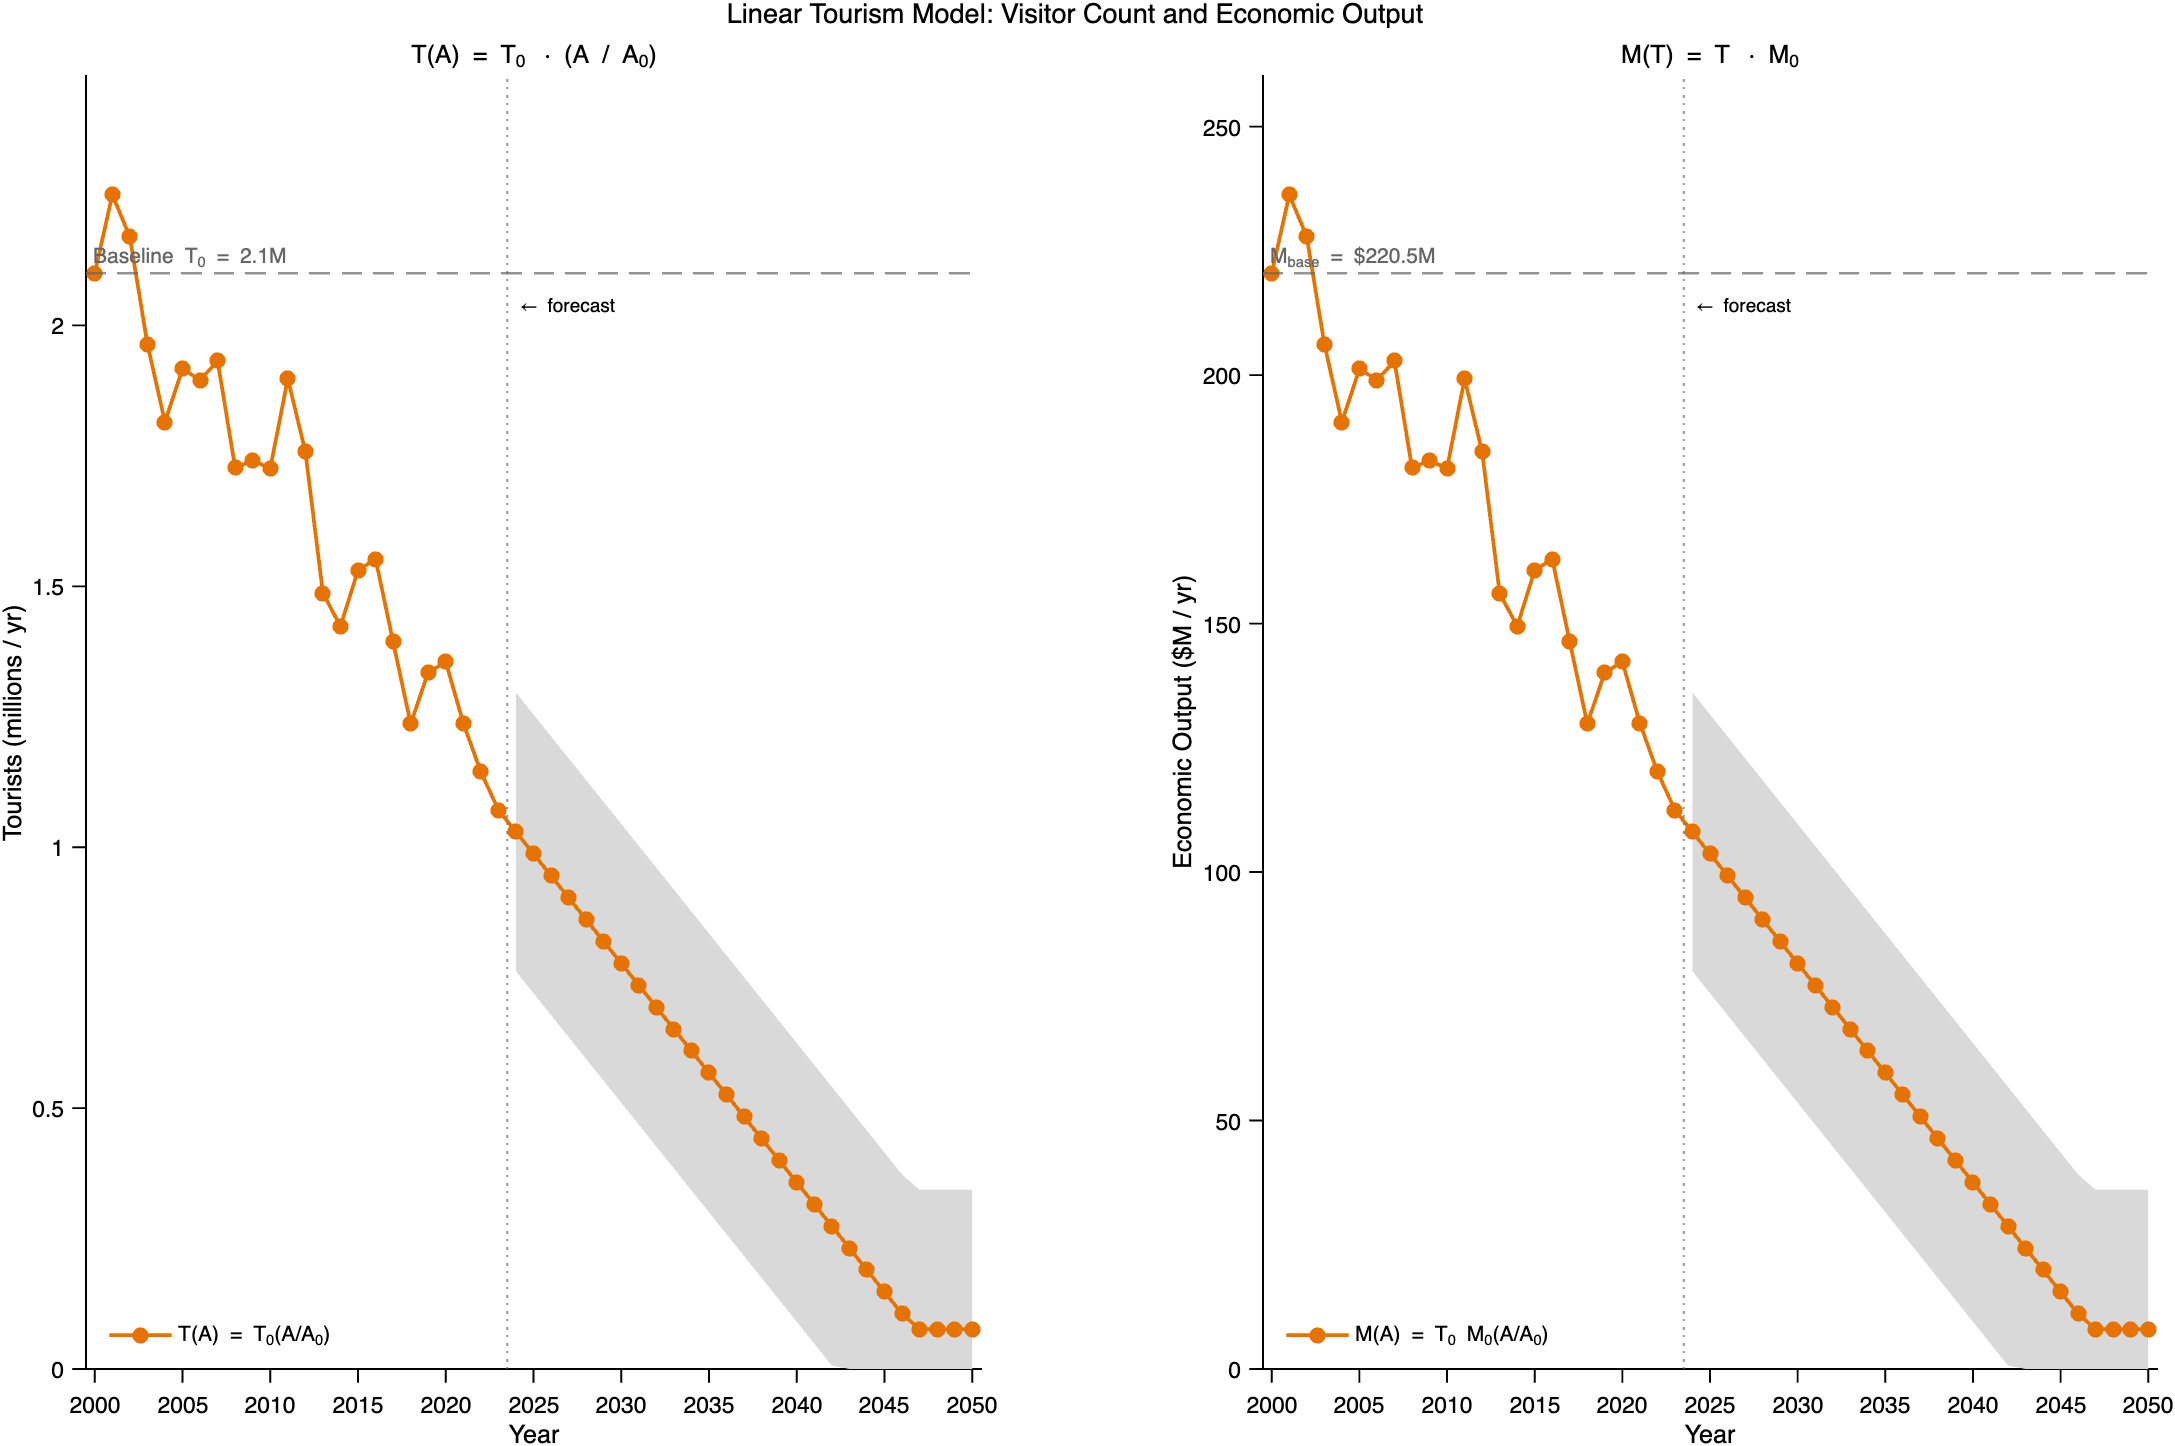
\includegraphics[width=\linewidth]{VisitorCountEconOutput.png}
        \caption{Linear tourism transfer function mapping hard coral cover to annual reef-dependent tourist arrivals under $T(A) = T_0 \cdot (A/A_0)$ (left) and corresponding annual economic output $M(T) = T \cdot M_0$ (right). The dashed reference line indicates baseline revenue $M_{\text{base}} = \$220.5$M per year.}
        \label{fig:tourism-model}
    \end{minipage}
    \hfill
    \begin{minipage}[t]{0.48\linewidth}
         \centering
    
\includegraphics[width=\linewidth]{Figures/CoralCovertoLoss.png}
    \caption{Annual economic losses decomposed by channel, showing wave damage and tourism loss as a stacked area chart with forecast total losses and 95\% CI (left), and all three series as individual lines over the full 2000--2050 horizon (right).}
        \label{fig:annual-losses}
    \end{minipage}
\end{figure}

\begingroup
\setstretch{1.2}
\renewcommand{\arraystretch}{1.1}
\rowcolors{2}{gray!15}{white}
\begin{xltabular}{\textwidth}{>{\centering\arraybackslash}p{1.0cm}
                             >{\centering\arraybackslash}p{2.0cm}
                             >{\centering\arraybackslash}X
                             >{\centering\arraybackslash}p{2.8cm}
                             >{\centering\arraybackslash}p{2.2cm}
                             >{\centering\arraybackslash}p{3.4cm}}
\rowcolor{white}\caption{Projected Annual Economic Losses from Coral Reef Degradation (Selected Years)}
\label{tab:economic-loss}\\
\toprule
\rowcolor{white}\textbf{Year} & \textbf{Benthic Cover (\%)} & \textbf{Wave Damage (\$M)} & \textbf{Tourism Loss (\$M)} & \textbf{Total Loss (\$M)} & \textbf{95\% CI (\$M)} \\
\midrule
\endfirsthead
\rowcolor{white}\multicolumn{6}{c}{\tablename\ \thetable{} -- \textit{continued from previous page}} \\[4pt]
\toprule
\rowcolor{white}\textbf{Year} & \textbf{Benthic Cover (\%)} & \textbf{Wave Damage (\$M)} & \textbf{Tourism Loss (\$M)} & \textbf{Total Loss (\$M)} & \textbf{95\% CI (\$M)} \\
\midrule
\endhead
\midrule
\rowcolor{white}\multicolumn{6}{r}{\textit{Continued on next page}} \\
\endfoot
\bottomrule
\endlastfoot
2024 & 13.49 & 685.6  & 112.4 & 798.0   & [665.9 -- 896.2]   \\
2026 & 12.39 & 710.9  & 121.2 & 832.2   & [711.5 -- 921.3]   \\
2028 & 11.29 & 733.1  & 130.1 & 863.2   & [753.3 -- 944.1]   \\
2030 & 10.19 & 752.5  & 138.9 & 891.4   & [791.4 -- 964.8]   \\
2035 & 7.44  & 790.0  & 160.9 & 950.9   & [872.5 -- 1008.9]  \\
2040 & 4.69  & 814.9  & 183.0 & 997.8   & [936.1 -- 1044.6]  \\
2045 & 1.94  & 830.6  & 205.0 & 1035.6  & [986.1 -- 1058.2]  \\
2050 & 1.00  & 834.3  & 212.5 & 1046.8  & [1000.6 -- 1058.2] \\
\end{xltabular}
\endgroup

\noindent Annual losses grow from approximately \$798 million in 2024 to \$1.05 billion per year by 2050, driven by the progressive loss of both tourism attractiveness and wave buffering capacity. The wave damage channel dominates in absolute terms throughout the forecast horizon, reflecting the high unit cost of coastal storm damage relative to per-tourist revenue; however, the tourism channel exhibits faster proportional growth as coral cover approaches the low-cover asymptote at which reef-dependent visitation effectively ceases. Discounted at $r = 1.5\%$ over 27 years, the total NPV of reef degradation costs is estimated at \$17.19 billion, decomposed as \$14.24 billion in wave damage and \$2.95 billion in tourism losses.

The sensitivity of total NPV losses to different intervention assumptions --- no action, holding current cover, and active restoration --- is evaluated in Section~4.2.

While the ARIMA and economic loss models capture the consequences of degradation already underway, understanding what drives acute bleaching events is equally critical for anticipating future shocks to coral cover. The following machine learning model characterizes those drivers directly from observational data.

\subsection{Pharmaceutical Option Value Model for Reef Biodiversity Loss}

Reef biodiversity loss risks harming not only marine organisms, but also humans and various economic sectors as described in the previous sections. This paper proposes a novel framework for analyzing the effects of biodiversity loss on the pharmaceutical industry, an idea conceptualized by prior literature, such as Simpson et al. (1996) and Costello \& Ward (2006), but not adequately explored in comparable reef risk analysis literature \cite{simpson1996, costello2006}. Fundamentally, the pharmaceutical industry stands to gain from reef remediation efforts due to past treatments for diseases like Alzheimer's and various forms of cancer being sourced from both coral and reef-hosted species, such as \textit{Cryptotethya crypta}. Therefore, facilitating reef remediation ensures that future treatments have a chance of being discovered, while continued degradation prevents any such chance of occurring at all.


The models used in this section draw inspiration from multi-dimensional analysis in graph and network theory with applications of multivariable calculus to analyze change over time. This provides a refined accurate approach for analyzing true pharmaceutical loss as a result of biodiversity decline compared to purely linear or single variable models.

The models described in previous sections, specifically those for wave energy and tourism, discuss effects directly caused by biodiversity loss. Pharmaceutical losses, however, are unrealized, and therefore hinge on reef remediation efforts, as continued reef degradation means these benefits will never be experienced. As described above, Simpson et al. and Costello \& Ward formed the basis of this section, with the former developing the initial framework for pharmaceutical bioeconomic risk analysis and the latter refining probability estimates.

\subsubsection{Species-Area Curve and Biodiversity Decline}

As hard coral cover declines along the SARIMAX-projected trajectory, effective reef habitat area $A(t)$ contracts proportionally, directly linking the benthic cover forecasts of Section~3.3 to this model. Species diversity at time $t$ is then estimated using the species-area relationship:

\begin{equation}
S(A,t) = c \cdot A(t)^{z}
\end{equation}

\noindent where $S$ is species count, $c$ is a region-specific scaling constant, and $z \approx 0.25$ is the power law exponent for reef systems \cite{macarthur1967}. $A(t)$ is derived by applying SARIMAX coral cover projections to each region's known reef area, producing a time-varying habitat area estimate for each of the seven modeled regions. The value $z = 0.25$ is a conservative literature-derived global average --- higher exponents documented in some reef systems would produce steeper species loss curves, reinforcing that this model's outputs represent a lower bound.

A particularly important feature of this formulation is its nonlinearity. The episodic near-zero cover years identified in the SARIMAX forecast --- most prominently 2028, 2036, 2044, and 2049 --- cause sharp contractions in $A(t)$ that propagate nonlinearly through the power law into disproportionately large species losses. This makes episodic bleaching events substantially more damaging to pharmaceutical option value than the gradual trend alone would suggest. Furthermore, species lost before pharmaceutical discovery are permanently removed from the pipeline regardless of subsequent restoration, distinguishing this loss channel from tourism and wave damage which remain theoretically recoverable under the restoration scenario evaluated in Section~4.2.

\subsubsection{Bioeconomic Prospecting Framework}

The framework used for bioeconomic prospecting in this paper is foundationally based on the work of Simpson et al., who modeled biodiversity value as expected return from pharmaceutical prospecting across species with heterogeneous discovery probabilities. The expected pharmaceutical value of a single species $s$ is given by:

\begin{equation}
\mathbb{E}[V(s)] = p(s) \cdot v(s)
\end{equation}

\noindent where the $(1 - p(s))$ term collapses to zero since a species yielding no active compound contributes nothing to the expected value. Discovery probability is defined as $p(s)$ in this paper, calibrated as:

\begin{equation}
p = \frac{N_{\text{approved}}}{N_{\text{screened}}} \cdot \phi_{\text{reef}}
\end{equation}

\noindent where $N_{\text{approved}}$ is the number of reef-derived approved compounds, $N_{\text{screened}}$ is the number of reef organisms screened in systematic programs, and $\phi_{\text{reef}} > 1$ is an upward adjustment factor reflecting the elevated bioactivity of reef organisms relative to the marine average, justified by the competitive chemical ecology of reef environments \cite{newman2016}. This yields an estimate of $p \approx 0.0001$ consistent with \cite{simpson1996, costello2006, newman2016}. However, $p(s)$ varied significantly across these sources --- Simpson et al.\ produced relatively conservative estimates due to a strict screening-to-approval ratio, while more recent work suggests higher hit rates for marine organisms specifically due to their unique evolutionary chemistry. Therefore, $p(s)$ should be considered a calibrated guide rather than a precisely fixed value.

The second component of the framework is $v(s)$, the expected NPV of a compound derived from species $s$ if it reaches clinical development, expressed as a probability-weighted discounted revenue expectation:

\begin{equation}
v = \sum_{k=1}^{K} \pi_k \cdot R_k \cdot e^{-\rho \tau_k}
\end{equation}

\noindent where $\pi_k$ is the probability of commercial outcome $k$, $R_k$ is the associated revenue, $\rho$ is the discount rate, and $\tau_k$ is the expected time from discovery to market \cite{costello2006}. The parameter values are calibrated against the observed record of reef-derived pharmaceutical approvals. Four reef-organism-derived compounds have reached clinical approval: AZT (peak annual revenue $\sim$\$400M), Ziconotide (\$50--100M annually), Trabectedin (\$150--200M annually), and Cytarabine (now generic, with substantial societal value captured through decades of standard leukemia treatment protocols). These four approvals span the full distribution of commercial outcomes, and together anchor $v(s)$ to a realistic expected value rather than a hypothetical upper bound.

Under the uniform $p(s)$ and $v(s)$ assumption necessitated by data limitations, the expected value over the full species pool at reef area $A$ and time $t$ simplifies to:

\begin{equation}
\mathbb{E}[V(A,t)] = \int_0^{S(A,t)} p(s) \cdot v(s) \, ds = p \cdot v \cdot S(A,t)
\end{equation}

\noindent confirming that under this simplification, expected pharmaceutical value scales linearly with species count at a given reef area and time. Treating $p(s)$ and $v(s)$ as uniform averages rather than species-specific values is a simplifying assumption that produces downward bias in the model's estimates and should be interpreted accordingly.

\subsubsection{Multi-Dimensional Cumulative Loss Function}
Cumulative pharmaceutical option value loss is expressed as a triple integral over time, reef area, and species distribution, mirroring the biomass loss integral in Equation~\ref{biomass-loss} of Section~3.2. The equation is given as:

\smallskip

\begin{equation}
\mathcal{L}_{\text{pharma}} = \int_0^T \int_0^{A(t)} \int_0^{S(A,t)} p(s) \cdot v(s) \, ds \, dA \, dt
\end{equation}

\smallskip

The innermost integral accumulates expected pharmaceutical option value loss across all species present in an area $A$ at time $t$, which is the bioeconomic prospecting value at a given spatial and temporal snapshot. The middle integral then aggregates this value spatially across the full reef extent at time $t$, which supports more species and therefore more pipeline value. The final integral $dt$ discounts cumulative losses until the year 2100, capturing all losses across the time horizon. Losses earlier in the time interval count more heavily towards the total NPV calculation consistent with the social discount rate $r=1.5\%$ applied throughout this paper.

Implementation of this equation in MATLAB required discretization into grids evaluated using nested trapezoidal summation. $A(t)$ was derived using SARIMAX coral cover projections, $S(A,t)$ from the species-area curve described above, and $p(s) \cdot v(s)$ was calibrated using literature values. This model differs from the others presented in this paper in that it is not a direct quantitative risk total of loss, but rather a lower-bound based on existing literature values. Therefore, the results of this section should be considered order-of-magnitude lower bounds rather than single-standing loss totals. Pharmaceutical NPV is added as a third channel alongside wave damage and tourism losses, increasing total status quo NPV and strengthening the cost-benefit case for the restoration program described in Section 5.

Unlike the tourism and wave damage channels, which grow gradually along the coral cover decline trajectory and remain theoretically recoverable under a restoration scenario, pharmaceutical option value lost during episodic near-zero cover years --- most prominently in 2028, 2036, 2044, and 2049 --- is permanently foreclosed. Species lost before discovery cannot be recovered by subsequent reef restoration regardless of the scale of intervention, making early action uniquely valuable for this channel relative to the others modeled in this paper.

The pharmaceutical option value model produces three principal outputs: cumulative discounted NPV losses across all seven regions under three discount rate assumptions, permanent option value foreclosed at episodic bleaching troughs, and a triple-integral integrand surface illustrating the spatial and temporal distribution of pharmaceutical value at risk.

\paragraph{Cumulative NPV Loss and Discount Rate Sensitivity.}
Figures~\ref{fig:pharma-npv-region} and ~\ref{fig:pharma-npv-sensitivity} present the cumulative discounted pharmaceutical option value loss under status quo degradation. The left panel decomposes losses by region, with the global total reaching approximately \$28~billion by 2100 at the baseline discount rate of $r = 1.5\%$. PRIA and Hawaii account for the largest regional contributions, driven by their high reef area and species scaling constants. The right panel replicates the global total across three discount rates ($r \in \{1.5\%, 3.0\%, 7.0\%\}$), confirming that the qualitative trajectory is preserved across all scenarios while higher rates compress the terminal NPV figure. The four bleaching trough years are annotated in the legend, and the accelerating loss rate between 2036 and 2044 reflects the compounding effect of successive near-zero cover events that prevent species recovery between disturbance cycles. These figures should be interpreted as conservative order-of-magnitude lower bounds, as the uniform $p(s)$ and $v(s)$ assumption suppresses heterogeneity in species bioactivity that would increase expected value under a fully specified model.

\paragraph{Permanent Option Value at Bleaching Troughs.}
Figure~\ref{fig:pharma-troughs} disaggregates annual pharmaceutical option value loss at each of the four episodic bleaching troughs into permanent and potentially recoverable components. The permanent component, conservatively estimated at 15\% of the annual trough loss, represents species driven to local extinction before pharmaceutical screening --- a loss that is irreversible regardless of subsequent reef restoration. Annual option value losses at the four troughs are \$0.426~billion (2028), \$0.612~billion (2036), \$0.772~billion (2044), and \$0.598~billion (2049). The increasing severity of the 2036 and 2044 troughs reflects the progressive reduction in recovery capacity as background cover declines toward the low-cover asymptote. Cumulatively, the permanent component across all four events represents pharmaceutical pipeline value that is foreclosed in perpetuity, distinguishing this channel from the tourism and wave damage losses which remain theoretically recoverable under the restoration scenario evaluated in Section~4.2.

\paragraph{Triple-Integral Integrand Surface.}
Figure~\ref{fig:pharma-surface} illustrates the discounted integrand $p \cdot v_{\text{life}} \cdot c \cdot A_{\text{eff}}^{z}$ as a function of both time $t$ and reef area fraction $A/A_{\max}$. The surface height --- denominated in \$B per year per unit area fraction --- declines monotonically from left to right as coral cover erodes and from front to back as discounting accumulates. The sharp ridgelines visible at the episodic trough years confirm that pharmaceutical value is not lost uniformly over time but is concentrated in acute disturbance events. This surface directly visualizes the integrand of $\mathcal{L}_{\text{pharma}} = \int_0^T \int_0^{A(t)} \int_0^{S(A,t)} p(s)\,v(s)\,ds\,dA\,dt$, and its rapid decay in the post-2044 period underscores the urgency of early intervention before successive bleaching events permanently compress the pharmaceutical prospecting frontier.


\begin{figure}[H]
    \begin{minipage}[c]{0.48\linewidth}
        \centering
        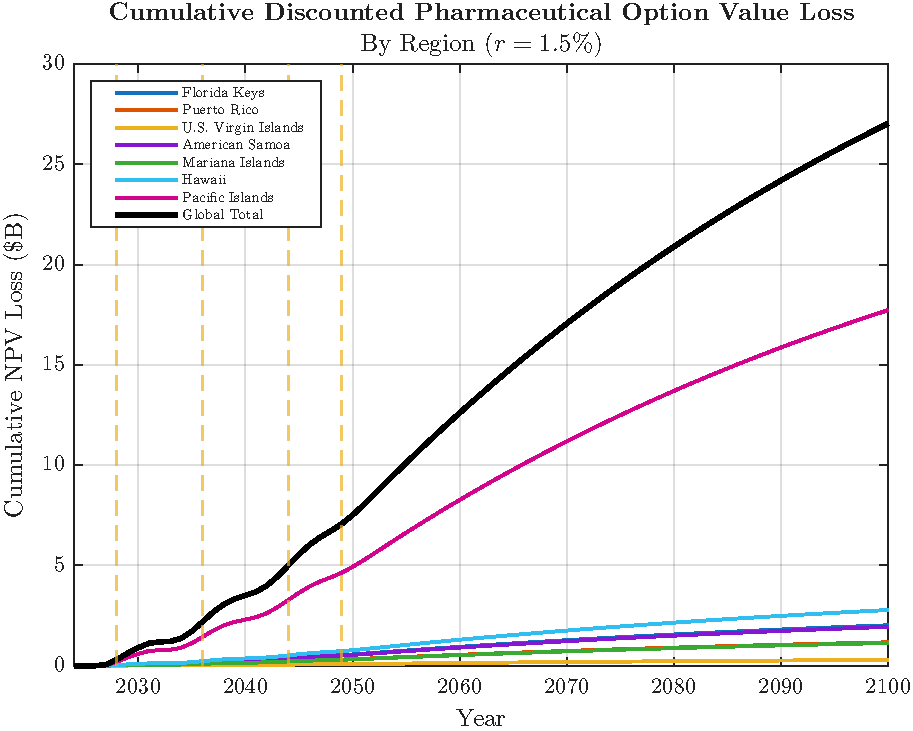
\includegraphics[width=\linewidth, height=6cm, keepaspectratio]{pharma_fig4a_cumulative_npv_by_region.pdf}
        \caption{Cumulative discounted pharmaceutical option value loss by region and global total ($r = 1.5\%$), 2024--2100. Pacific Islands dominates losses owing to its greater reef extent and species richness.}
        \label{fig:pharma-npv-region}
    \end{minipage}
    \hfill
    \begin{minipage}[c]{0.48\linewidth}
        \centering
        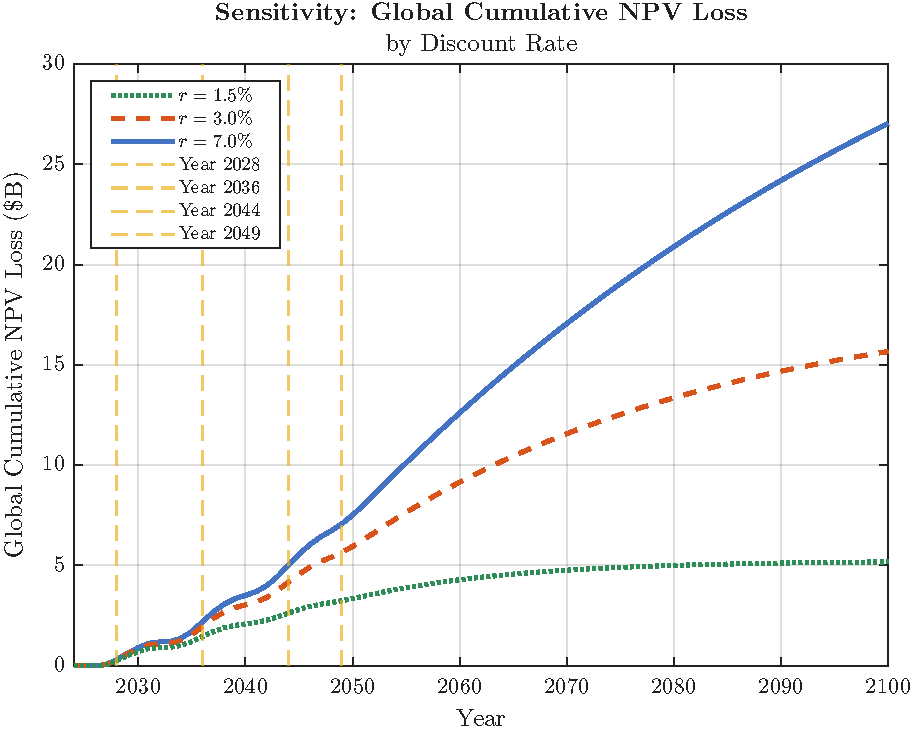
\includegraphics[width=\linewidth, height=6cm, keepaspectratio]{pharma_fig4b_sensitivity_discount_rate.pdf}
        \caption{Global cumulative NPV loss under discount rates of 1.5\%, 3.0\%, and 7.0\%. Terminal losses range from $\sim$\$28~billion at $r = 1.5\%$ to $\sim$\$9~billion at $r = 7.0\%$, illustrating strong sensitivity to the social discount rate.}
        \label{fig:pharma-npv-sensitivity}
    \end{minipage}
\end{figure}

\begin{figure}[H]
    \begin{minipage}[c]{0.48\linewidth}
        \centering
        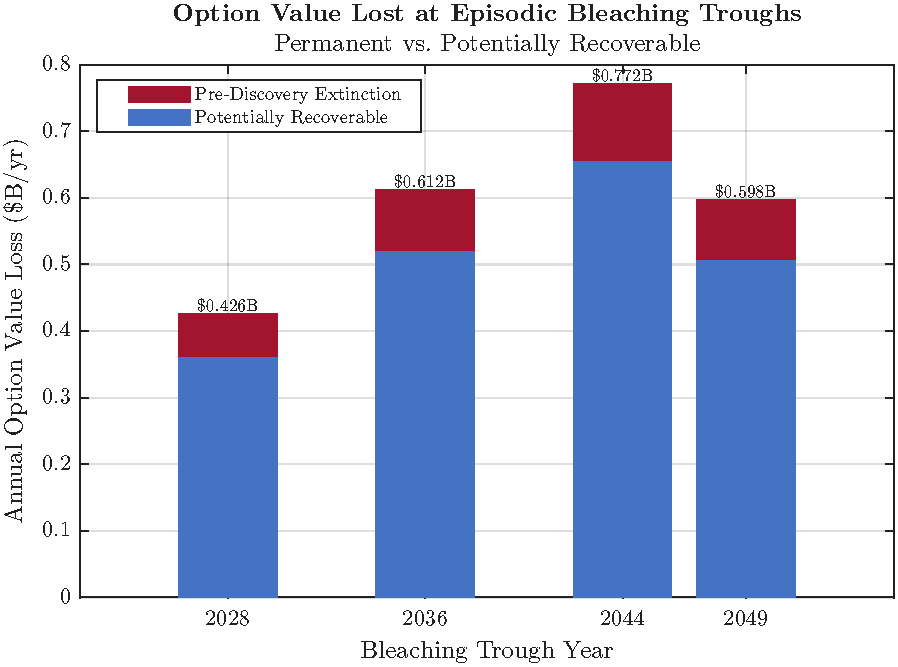
\includegraphics[width=\linewidth, height=6cm, keepaspectratio]{pharma_fig5_trough_loss_3.pdf}
        \caption{Annual pharmaceutical option value lost at each bleaching trough, split into recoverable and permanent (pre-discovery extinction) components. The 2044 trough produces the largest single-year loss at \$0.772~billion.}
        \label{fig:pharma-troughs}
    \end{minipage}
    \hfill
    \begin{minipage}[c]{0.48\linewidth}
        \centering
        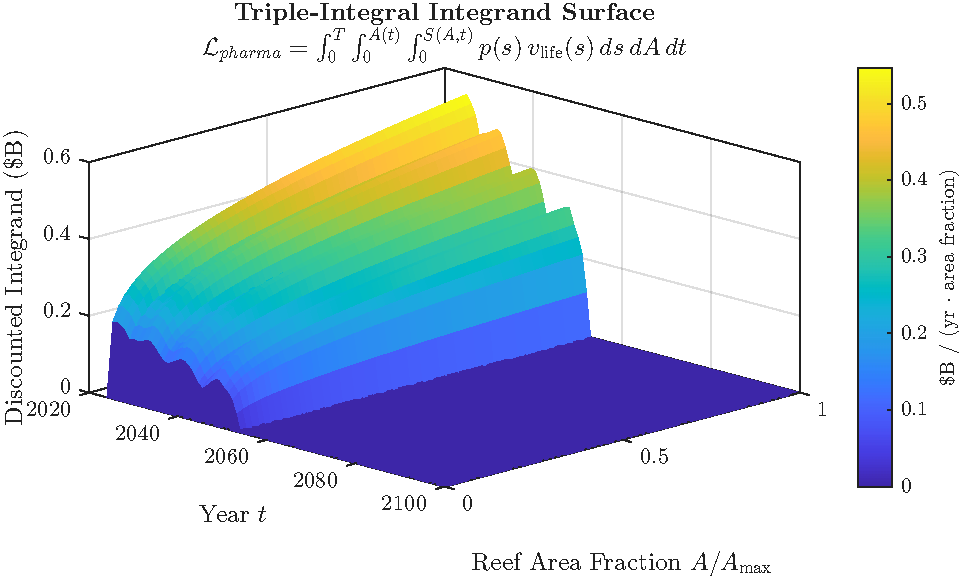
\includegraphics[width=\linewidth, height=6cm, keepaspectratio]{pharma_fig6_triple_integral_2.pdf}
        \caption{Triple-integral integrand surface of discounted pharmaceutical option value density as a function of time and reef area fraction. Ridgelines at bleaching trough years highlight the concentration of irreversible losses in acute disturbance events.}
        \label{fig:pharma-surface}
    \end{minipage}
\end{figure}

\section{Risk Analysis}

The Risk Analysis characterizes the severity, likelihood, uncertainty, expected value, and distribution
of risks associated with coral reef degradation, drawing on the models described in Section 3. Severity is
quantified through projected economic losses from the Gordon-Schaefer and economic loss models; likelihood
is expressed through Monte Carlo collapse probabilities; uncertainty is captured via confidence intervals on
all forecasts; expected value of loss is reported as net present value; and the distribution of outcomes is
described through the stochastic simulation results. The Risk Analysis also evaluates all three categories of
risk mitigation strategy — insurance mechanisms, behavior changes, and strategies to modify outcomes —
in preparation for the recommendations in Section 5. Statistical and sensitivity analyses are included where
necessary.

\subsection{Results and Implications}

\subsubsection{Gordon-Schaefer Model}
The results of the Gordon-Schaefer Model show a variety of critical metrics that are important for future policy. Firstly, the model's results show a stark difference between global losses directly from degradation and those from biomass loss. Specifically, global losses due to degradation stem from damage to existing reef infrastructure, while losses from biomass span losses across the fishing industry. The latter is a more holistic measure of the fishing industry because it captures the Level II effects described earlier, while the losses from degradation only capture Level I Effects. 

These findings describe the severity of Level II Effects and their capability to proliferate across different industries and sectors. Across all regions analyzed in this paper, a total impact of \$4 billion was assessed strictly from losses incurred by the fishing industry. Furthermore, the model showed extremely high biomass losses for regions with low reef area, such as the Virgin Islands and Mariana Islands, suggesting that reef area is only part of the economic impact associated with reef degradation. Other factors such as economic dependencies on the reef, including those from fishermen, compound effects on smaller reefs to have global impacts of extremely high magnitudes.

The Gordon-Schaefer results quantify the fishery losses driven by reef degradation, but the full economic picture requires accounting for the two additional channels, tourism revenue and coastal wave protection, that are most directly sensitive to the hard coral cover trajectory projected by the ARIMA and SARIMAX models.

\subsubsection{ARIMA, SARIMAX, and Economic Loss Model}
The ARIMA and SARIMAX forecasts confirm a statistically significant long-run decline in hard coral cover of $-0.6397\%$ per year after controlling for depth, algae cover, and marine protection status. The most critical finding from these models is not the gradual trend itself, but the emergence of episodic near-zero cover years at four-year intervals, most prominently in 2028, 2036, 2044, and 2049, which correspond directly to the bleaching cycle frequencies identified in the Random Forest model. The SARIMAX model, which conditions on the projected algae trajectory, projects a more severe outlook than the ARIMA alone, with cover approaching zero percent in both 2036 and 2044. This is consistent with the Level I and Level II effects described in Table 1: as algae continues to displace hard coral, the aesthetic and structural value of the reef declines simultaneously, compounding losses across both the tourism and wave protection channels.

The economic loss model translates these cover projections into quantified annual losses, growing from \$798 million in 2024 to \$1.05 billion per year by 2050. The wave damage channel dominates throughout, reflecting the high cost of losing the coastal protection that reefs provide, the same 97\% wave energy absorption described in Section 1, while the tourism channel accelerates proportionally as cover approaches the low-cover asymptote. Critically, the 27-year NPV of \$17.19 billion under the status quo represents a lower bound, as the model is parameterized on the Florida Keys alone. Regions with greater economic dependence on reef-based tourism, such as Small Island Developing States not captured in this dataset, would produce substantially higher aggregate figures. The sensitivity analysis in Section 4.2 confirms that even partial intervention, holding cover constant rather than restoring it, cuts this NPV loss by nearly \$3 billion, underscoring that the economic case for reef conservation is robust even under conservative assumptions.

While the ARIMA and economic loss models project the aggregate financial consequences of continued degradation, the bleaching model below identifies the specific thermal conditions that drive the acute cover losses underlying those projections. This provides a mechanistic explanation for the episodic low-cover years the forecast captures.

\subsection{Sensitivity Analysis}

To assess the responsiveness of the economic loss model to intervention assumptions, three scenarios are evaluated under the NPV framework. This analysis tests how total projected losses change when the key input assumption, the trajectory of future coral cover, is varied across plausible intervention states, providing actionable benchmarks for policy and conservation investment.

The first scenario, Status Quo, assumes no intervention and represents the full \$17.19 billion loss estimated in Section~3.4. The second, Hold Cover, assumes that active management is successful in preventing any further decline from current levels, yielding an NPV of \$14.29 billion and a net saving of \$2.90 billion relative to the status quo. The third, Restoration, assumes an active program that partially restores coral cover toward historical reference levels, yielding an NPV of \$9.11 billion and a net saving of approximately \$8.08 billion. These results are summarized in Table 14.

\begingroup
\setstretch{1.2}
\renewcommand{\arraystretch}{1.1}
\rowcolors{1}{gray!15}{white}
\begin{xltabular}{\textwidth}{>{\centering\arraybackslash}p{4.8cm}
                >{\centering\arraybackslash}p{2.3cm}
                >{\centering\arraybackslash}X}
\rowcolor{white}\caption{Net Present Value of Economic Losses Under Mitigation Scenarios}
\label{tab:mitigation-npv}\\
\toprule
\rowcolor{white}\textbf{Scenario} & \textbf{NPV (\$M)} & \textbf{Savings vs.\ Status Quo (\$M)} \\
\midrule
\endfirsthead
\rowcolor{white}\multicolumn{3}{c}{\tablename\ \thetable{} -- \textit{continued from previous page}} \\[4pt]
\toprule
\rowcolor{white}\textbf{Scenario} & \textbf{NPV (\$M)} & \textbf{Savings vs.\ Status Quo (\$M)} \\
\midrule
\endhead
\midrule
\rowcolor{white}\multicolumn{3}{r}{\textit{Continued on next page}} \\
\endfoot
\bottomrule
\endlastfoot
Status Quo (no intervention)  & \$17{,}190.4 & ---         \\
Hold Cover                    & \$14{,}289.1 & \$2{,}901.3  \\
Restoration                   & \$9{,}114.6  & \$8{,}075.8  \\
\end{xltabular}
\endgroup

\noindent The magnitude of savings under the Restoration scenario, more than \$8 billion relative to status quo, establishes a compelling economic upper bound on the value of large-scale reef restoration investment. Even the more modest Hold Cover scenario, which requires only that current degradation be halted rather than reversed, yields savings of nearly \$2.9 billion. These findings confirm that the economic loss model is highly sensitive to the assumed trajectory of coral cover, and that even partial intervention produces non-linear improvements in expected outcomes relative to inaction. The figures below plot the cumulative discounted loss trajectory alongside the mitigation scenario comparison.

\begin{figure}[H]
    \begin{minipage}[t]{0.48\linewidth}
       \centering
    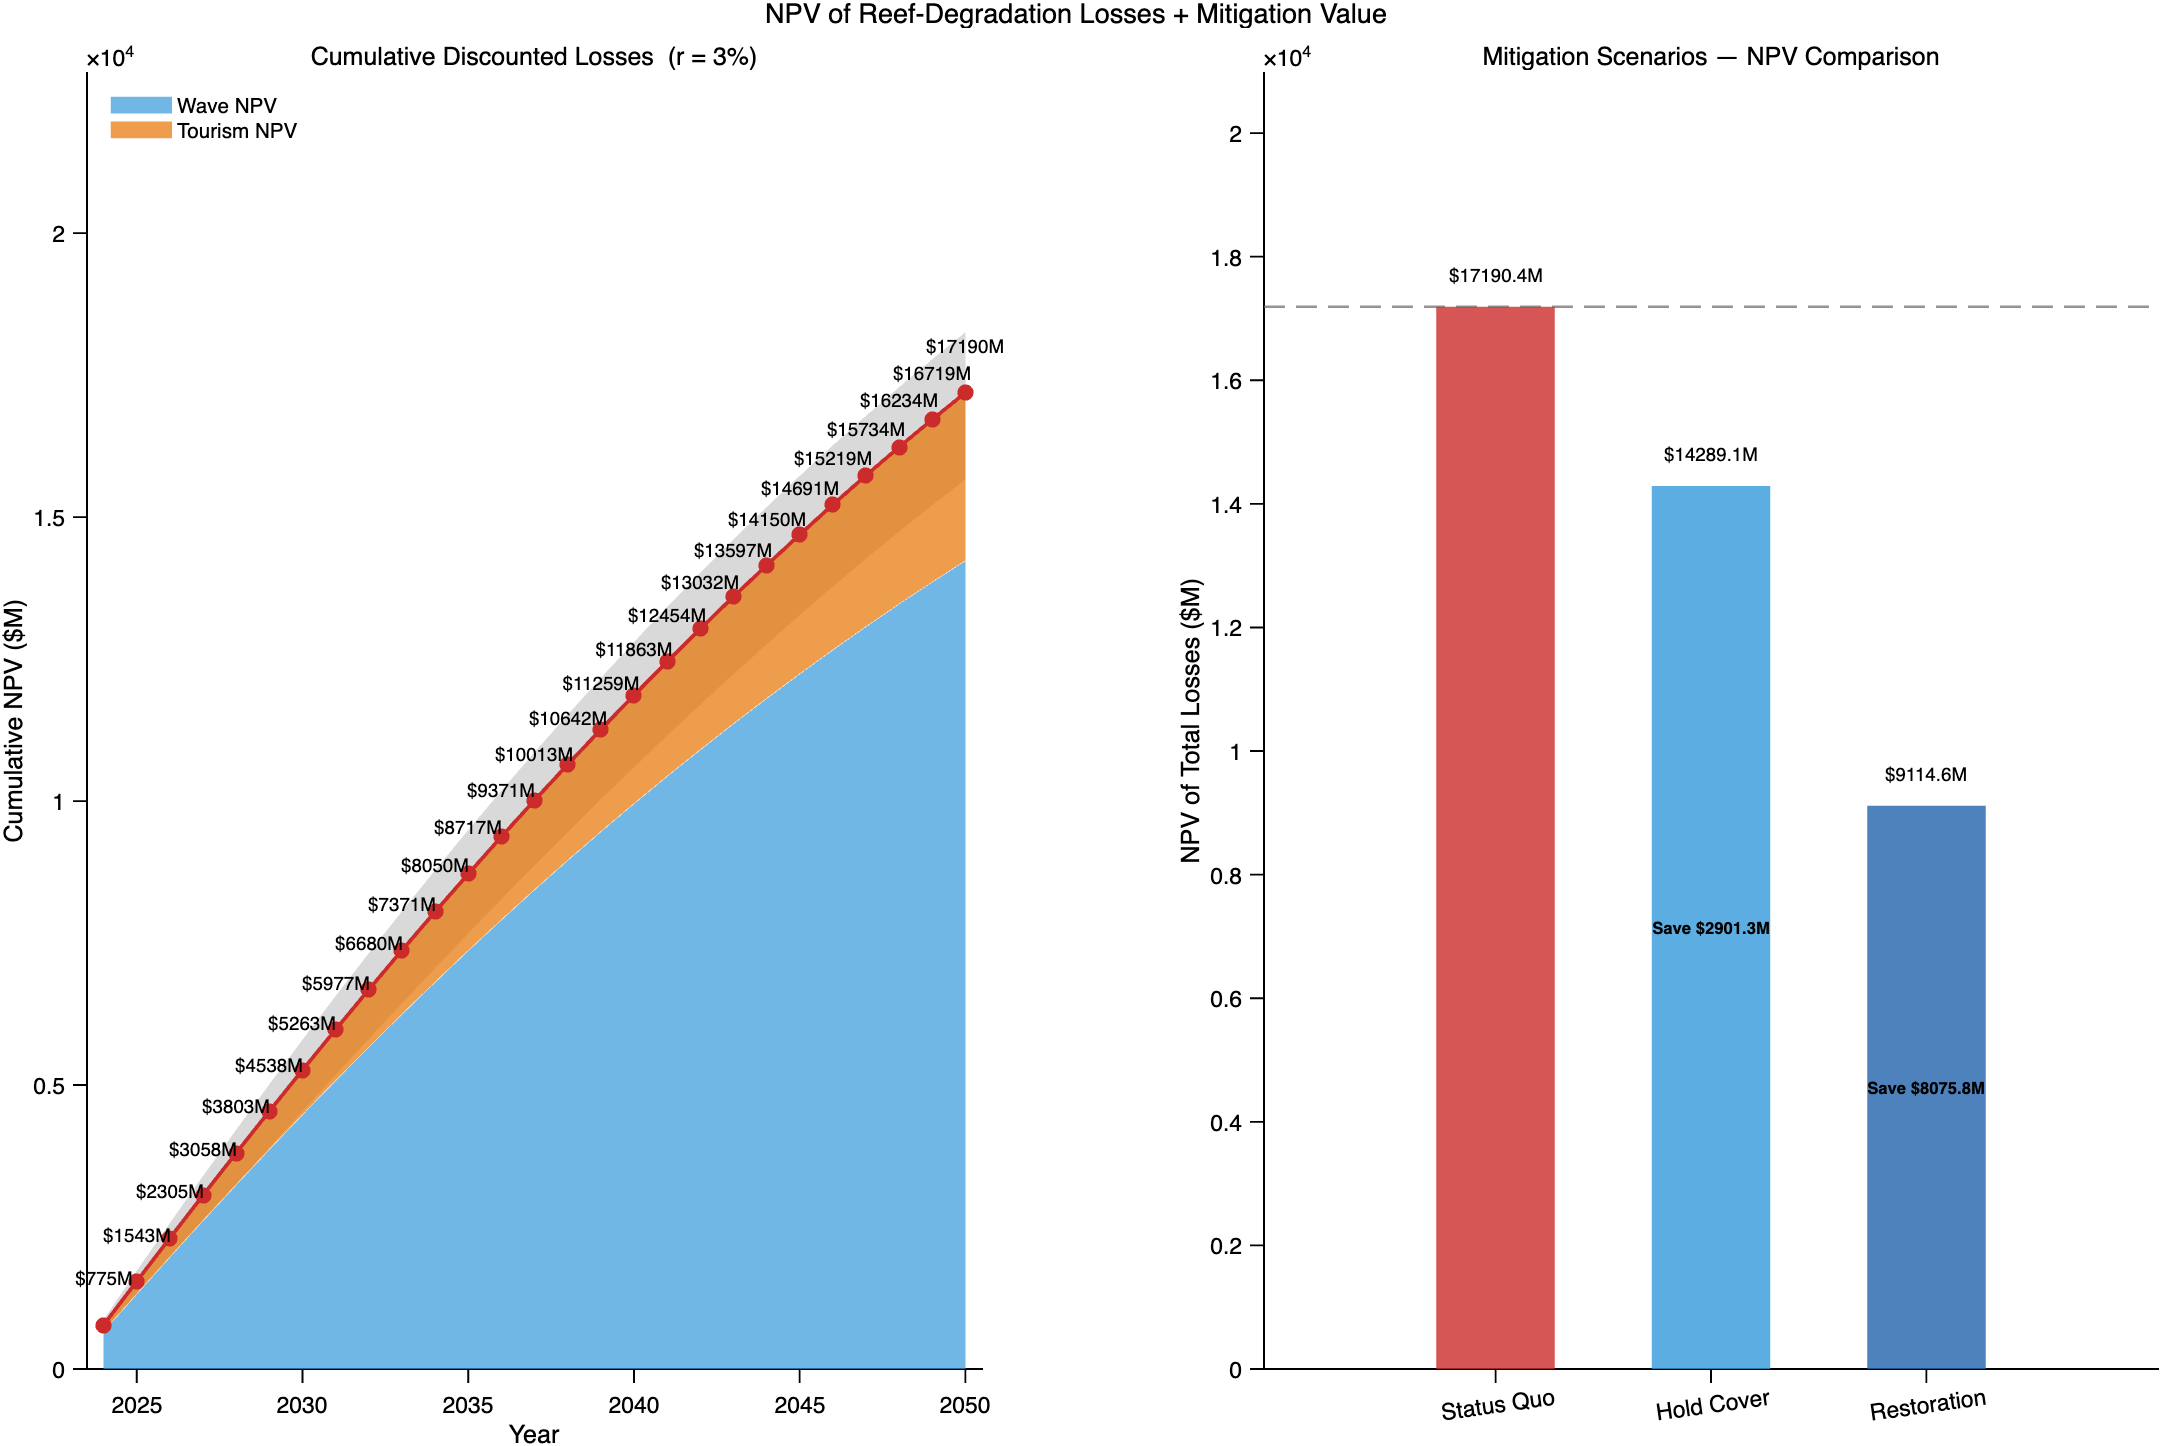
\includegraphics[width=\linewidth]{Figures/NPVofLoss+MitigationVal.png}
    \caption{Cumulative discounted NPV of wave damage and tourism losses with 95\% CI (left), and total NPV under Status Quo, Hold Cover, and Restoration scenarios with annotated savings relative to baseline (right).}
    \label{fig:npv-mitigation}
    \end{minipage}
    \hfill
    \begin{minipage}[t]{0.48\linewidth}
        \centering
    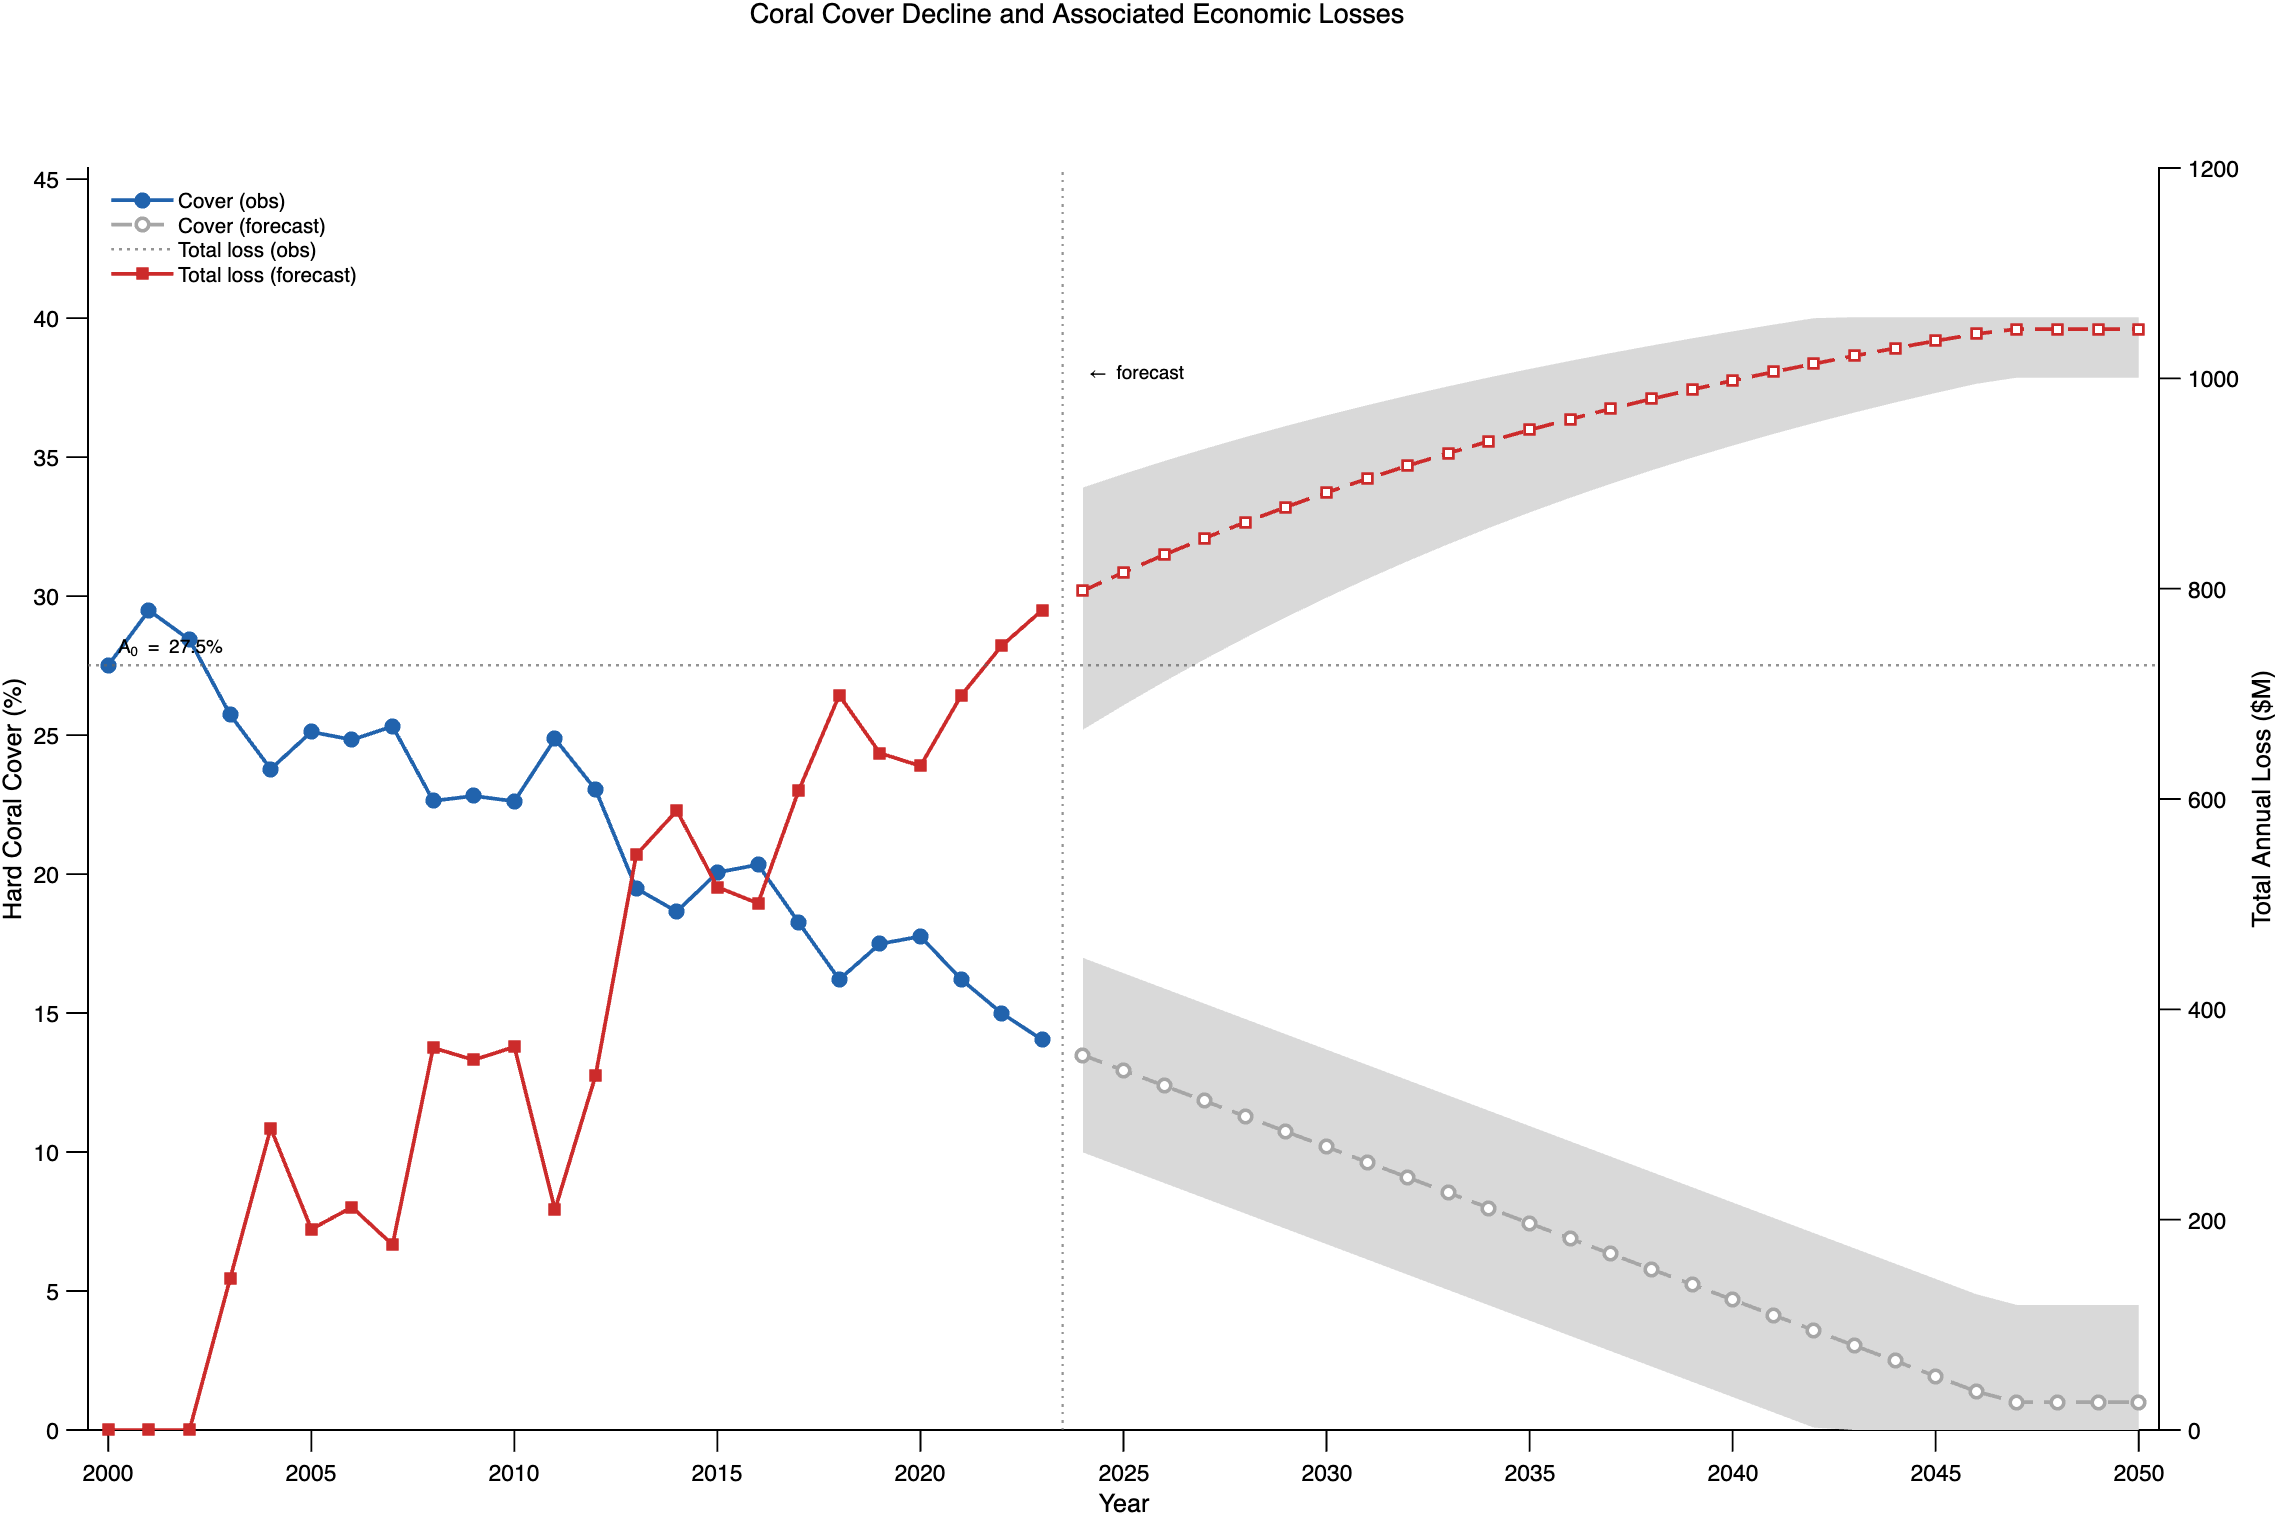
\includegraphics[width=0.85\linewidth]{Figures/CoverDeclintoOverallLoss.png}
    \caption{Dual-axis comparison of hard coral cover decline and total annual economic loss over the full time series. Observed values shown as solid lines; forecasts as dashed lines with 95\% prediction interval shaded.}
    \label{fig:cover-vs-loss}
    \end{minipage}
\end{figure}

While this model uses $r = 1.5\%$ as its baseline discount rate per OMB Circular A-4 intergenerational guidance \cite{omb_a4_2003}, the full OMB range also includes rates of $3\%$ and $7\%$. Figure 11 replicates the scenario analysis across all three rates to confirm that the intervention conclusions are not sensitive to this choice. As expected, higher discount rates compress the cumulative NPV estimates --- the status quo loss falls from \$6,449M at $r = 1.5\%$ to \$3,052M at $r = 7\%$ --- but the ranking of scenarios is preserved at every rate: Restoration always dominates Hold Cover, which always dominates Status Quo. Figure 12 further tests model robustness via a tornado analysis, varying the three most influential parameters by $\pm50\%$. The coastal damage ceiling $D_{\max}$ produces the widest output range (\$4,298M), followed by the wave attenuation coefficient $k$ (\$3,832M) and per-tourist output $M_0$ (\$2,245M), consistent with the wave damage channel accounting for 67\% of baseline NPV losses.

\begin{figure}[H]
    \begin{minipage}[t]{0.48\linewidth}
        \centering
        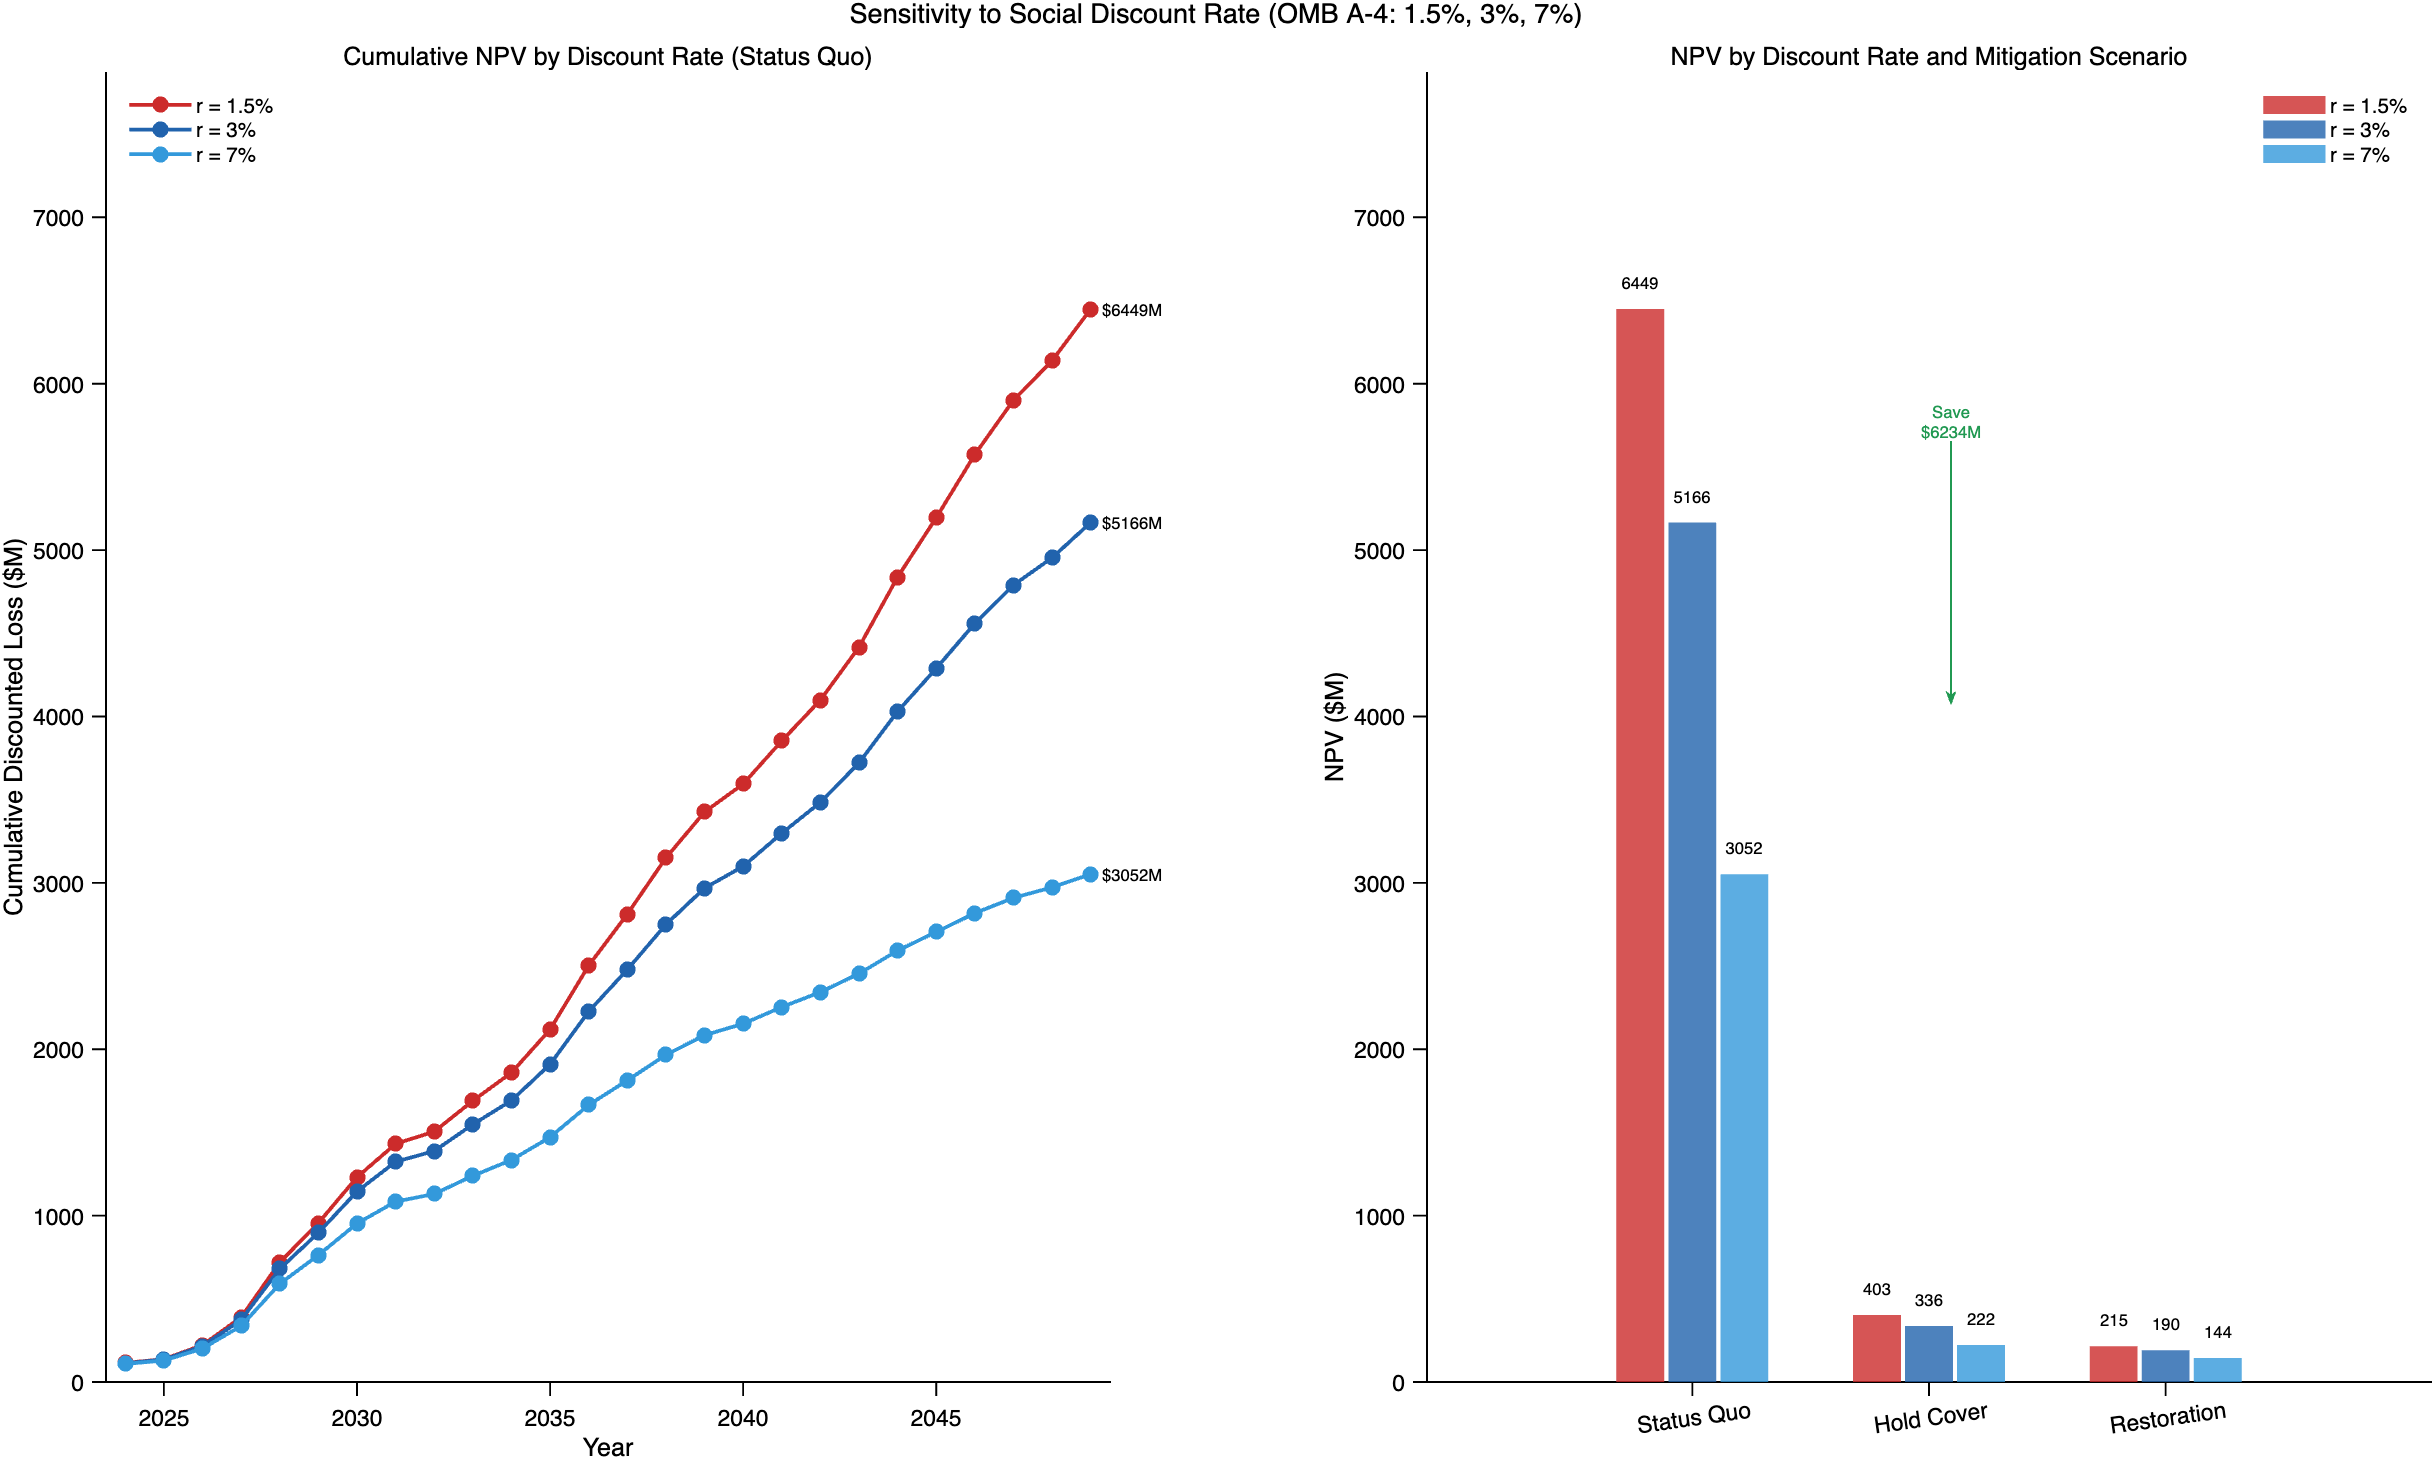
\includegraphics[width=\linewidth]{Figures/SA_Discount.png}
        \caption{Cumulative NPV loss trajectories under Status Quo (left) and terminal NPV by scenario (right) across discount rates $r = 1.5\%$, $3\%$, and $7\%$. Scenario ordering is preserved across all rates, with Restoration consistently producing the lowest total loss.}
        \label{fig:sa-discount}
    \end{minipage}
    \hfill
    \begin{minipage}[t]{0.48\linewidth}
        \centering
        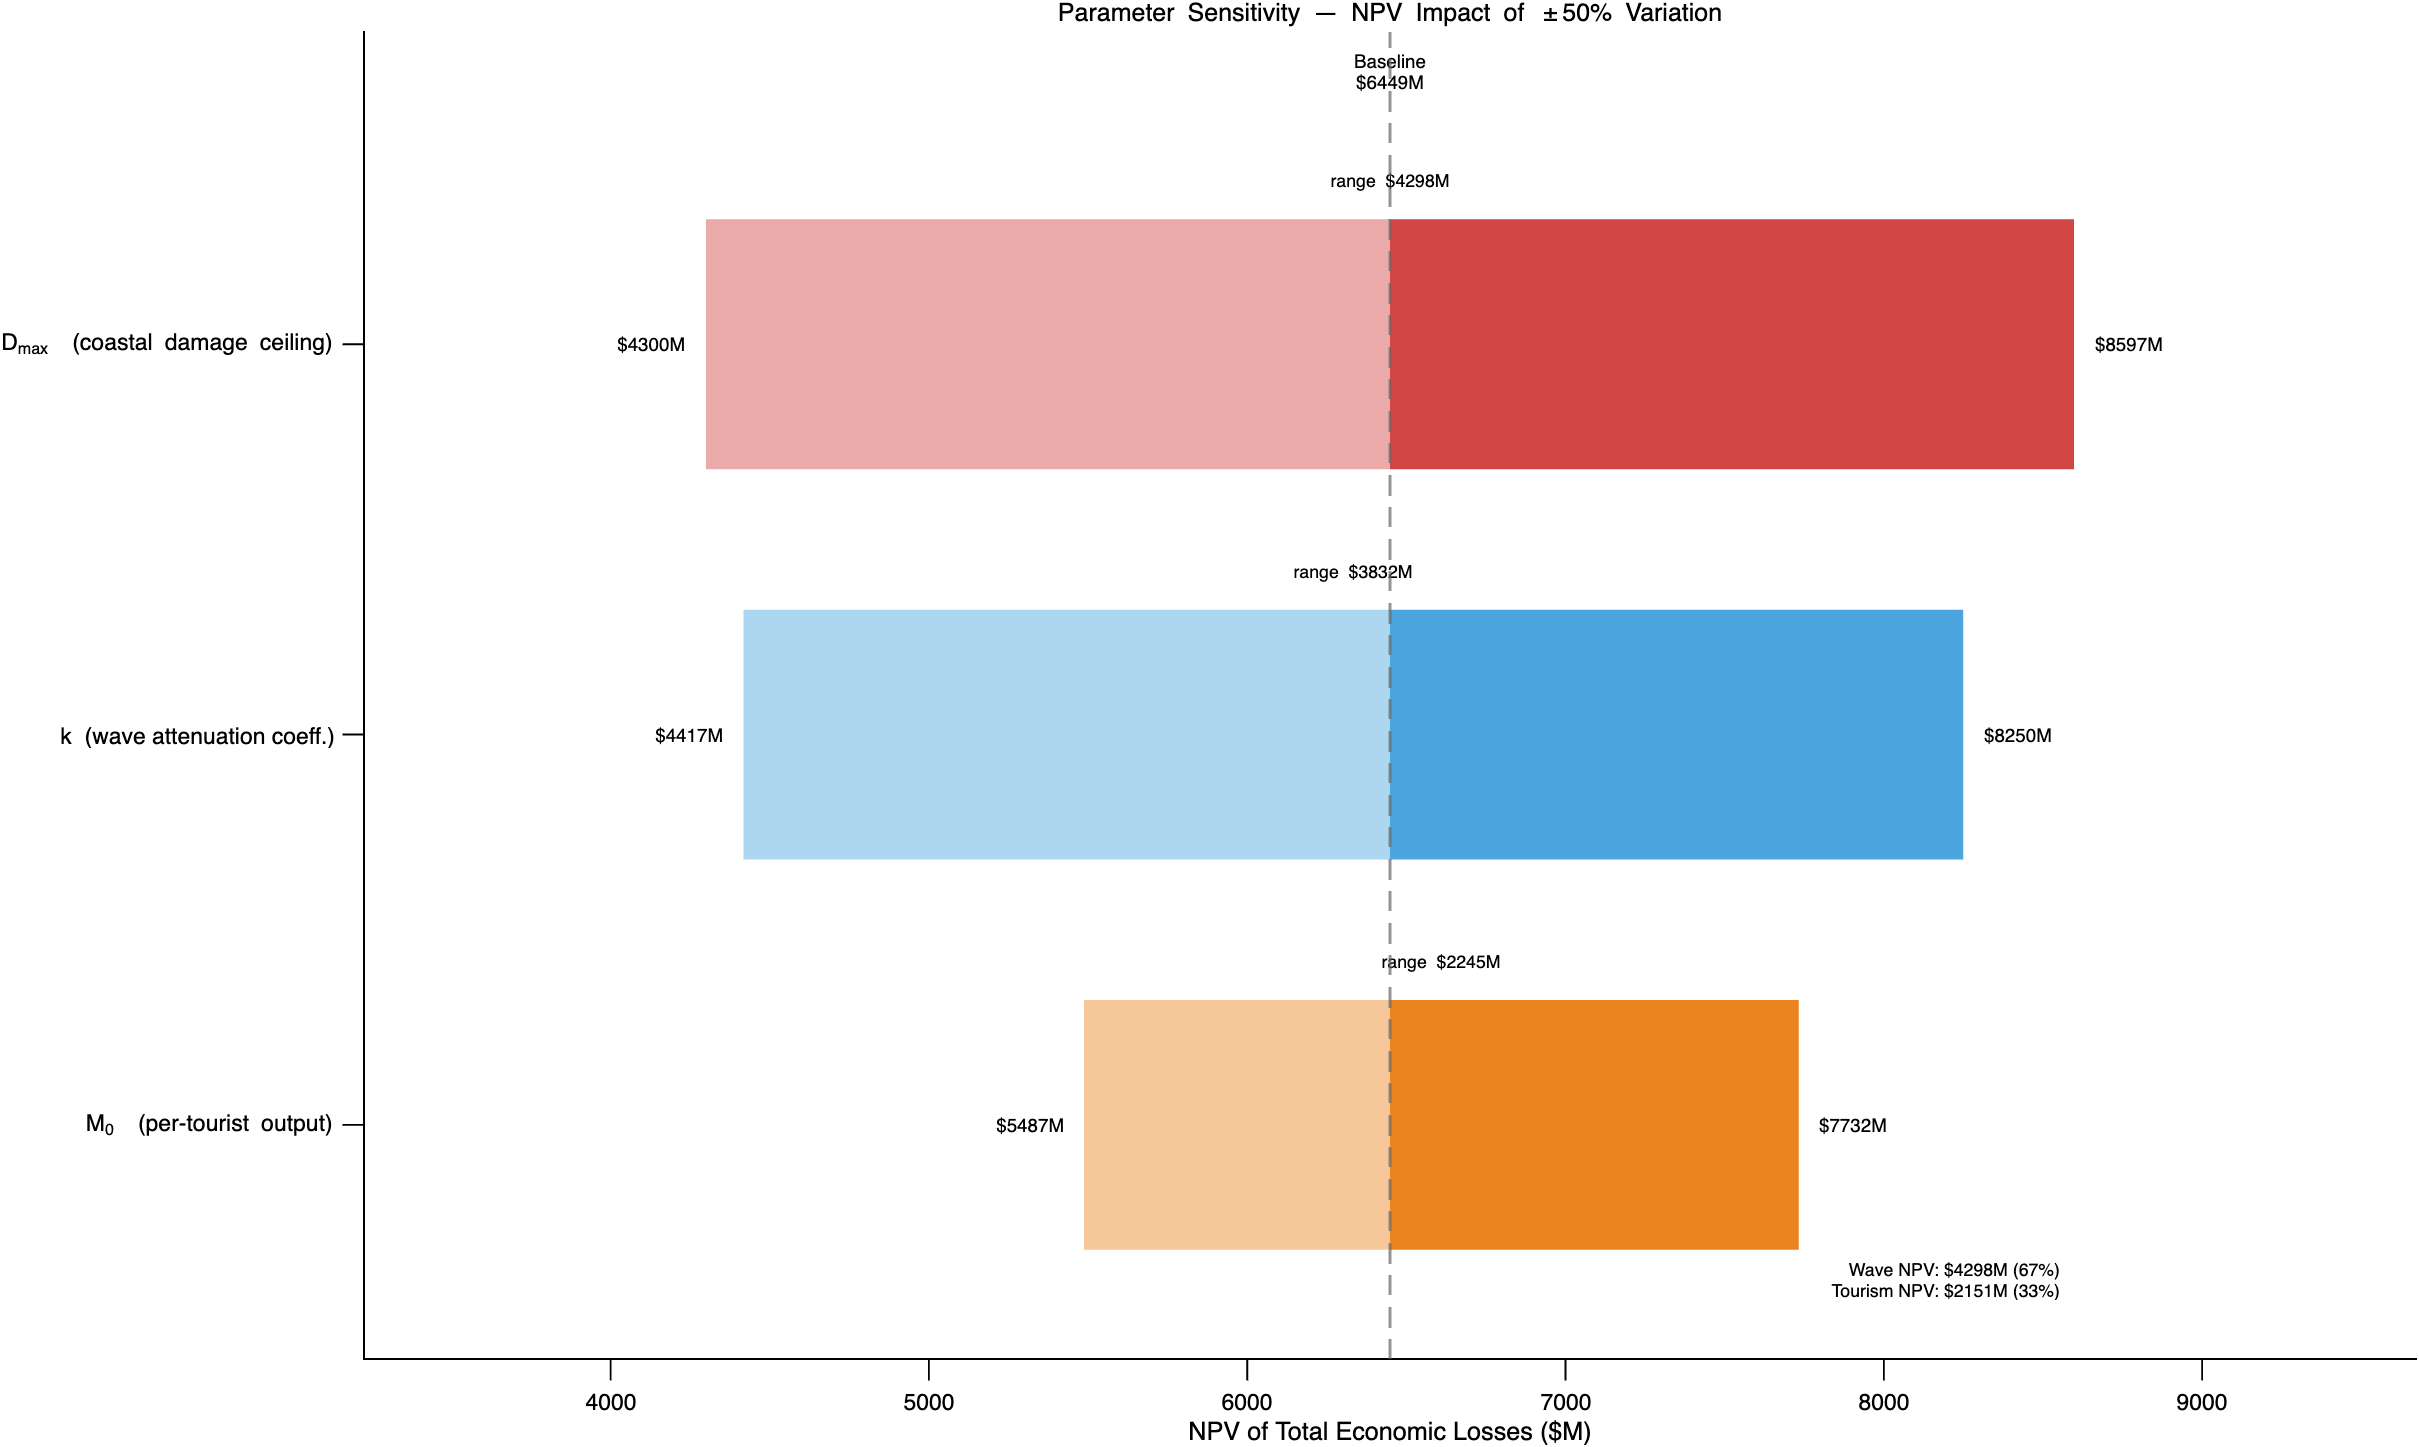
\includegraphics[width=\linewidth]{Figures/SA_Tornado.png}
        \caption{Tornado diagram showing sensitivity of the baseline NPV estimate (\$6,449M) to $\pm50\%$ variation in $D_{\max}$ (range \$4,298M), $k$ (range \$3,832M), and $M_0$ (range \$2,245M). The dashed vertical line marks the baseline NPV.}
        \label{fig:sa-tornado}
    \end{minipage}
\end{figure}

These estimates have direct implications for how insurers, governments, and conservation organizations should evaluate the cost-effectiveness of reef protection relative to the escalating damages that continued degradation will impose on coastal communities and reef-dependent industries.

\section{Recommendations}
The recommendations proposed in this paper address all three categories of risk mitigation strategy:
insurance mechanisms (Program~4), behavior changes (Programs~3 and~5), and strategies to modify
outcomes through direct reef restoration (Programs~1 and~2). These recommendations take the form of
government subsidies and rebates, environmental conservation policy, and an insurance reserve, and are
divided into individual programs at varying scales concerning different aspects of reef degradation,
including social and economic incentives. Each program is directly motivated by quantified model
outputs: the Gordon-Schaefer collapse probabilities exceeding 97\% across all regions, the
$-0.6397\%$ per year benthic cover decline confirmed by the SARIMA panel regression, the
$\$17.19$ billion 27-year NPV loss under the status quo, and the sensitivity analysis demonstrating
that active restoration recovers \$8.08 billion in avoided losses. Together, these five programs
represent a forward-looking risk management strategy designed to shift the economic trajectory from
the status quo collapse curve toward the Restoration scenario modeled in Section~4.2.

\subsection{Economic Incentives}
Government subsidies and rebates are common forms of economic incentives to drive changes in behavior
in free market economies. These policies are often instituted by the central government and last for a
set period of time. Common examples of recent government subsidies include the clean energy incentives
as part of the Inflation Reduction Act passed in 2022 and lasting until ten years later. The main
impacts of reef degradation until 2100 concern the fishing industry and tourism. These industries pose
fundamentally separate business models and will therefore be addressed using different policy approaches.

\subsubsection{Fishing Policy}

The impact of reef degradation on global fishing from the 7 regions analyzed in this paper exceeds
\$4 billion until the year 2100. This, coupled with an increased density of reefs in regions that were
not explored in this paper, such as Oceania, indicate extremely high economic impacts on the fishing
industry and the economies of Small Island Developing States (SIDS). This poses a severe problem, as
decreased revenue from fishing means lower wages for fishermen, only accelerating and prolonging
recessionary periods in these states. To mitigate these concerns, the proposed recommendations for
local fisheries and governments in these states are as follows.

\begingroup
\setstretch{1.2}
\renewcommand{\arraystretch}{1.1}
\rowcolors{1}{gray!15}{white}
\begin{xltabular}{\textwidth}{>{\centering\arraybackslash}p{2.2cm} 
                >{\centering\arraybackslash}p{2.4cm}
                >{\centering\arraybackslash}p{2.4cm}
                >{\centering\arraybackslash}X}
\rowcolor{white}\caption{Fishing Policy Recommendations for Governments}
\label{tab:fishing-policy}\\
\toprule
\rowcolor{white}\textbf{Policymakers} & \textbf{Stakeholders} & \textbf{Policy Type} & \textbf{Policy and Justification} \\
\midrule
\endfirsthead
\rowcolor{white}\multicolumn{4}{c}{\tablename\ \thetable{} -- \textit{continued from previous page}} \\[4pt]
\toprule
\rowcolor{white}\textbf{Policymakers} & \textbf{Stakeholders} & \textbf{Policy Type} & \textbf{Policy and Justification} \\
\midrule
\endhead
\midrule
\rowcolor{white}\multicolumn{4}{r}{\textit{Continued on next page}} \\
\endfoot
\bottomrule
\endlastfoot
Governments & Fisheries & Subsidy & Providing provisions to support transitions to new equipment and fishing approaches, given that reef fish populations are set to decrease heavily. A rebate of around 50\% on gear sales would prove extremely effective. \\
Governments & Environmental Agencies & Conservation & Assigning the reefs with the highest risk of fish populations reaching the critical threshold as Marine Protected Areas (MPAs) will allow fish populations to recover sustainably. \\
Governments & Fisheries & Tax Credit & Granting fisheries tax credits for coral restoration would incentivize conservation and remediation. Current programs already exist, but funding is an issue. \\
\end{xltabular}
\endgroup

The recommendations outlined in Table~15 provide a general overview of risk mitigation strategies,
ranging from government subsidies to environmental conservation policy. As shown in the ARIMA and
SARIMAX models, the most critical next step for local legislatures is focusing on reef restoration as
opposed to curbing current degradation, which consists of government programs intended to increase
reef cover rather than maintain its current level into the future. Critically, the sensitivity analysis
in Section~4.2 confirms that the Restoration scenario saves \$8.08 billion in NPV losses compared to
only \$2.90 billion under the Hold Cover scenario, meaning that every year of inaction forfeits a
growing share of this recoverable value as coral cover approaches the episodic near-zero troughs
projected in 2028, 2036, and 2044. Given in Table~16 is a cost-benefit analysis conducted using the
outputs of the Stochastic Gordon-Schaefer Model to determine the optimal government subsidy packages
to aid in reef remediation.

\subsubsection{Tourism Policy}

Tourism is the second major economic channel affected by reef degradation, with the economic loss model
projecting \$2.95 billion in NPV tourism losses through 2050 under the status quo scenario. While the
scope of this project does not lend itself to tourism-specific subsidies in the same way as the fishing
industry, the recommendations in this paper address the tourism stakeholder group through existing
programs. Program~1 (Coral Reef Restoration) directly protects reef-dependent visitation revenue by
maintaining and recovering the hard coral cover that drives tourist arrivals; the linear tourism model
in Section~3.4 shows that each percentage point of recovered cover translates proportionally to
recovered visitor arrivals and revenue relative to the \$220.5 million per year baseline. Program~5
(MPA Monitoring) preserves the aesthetic value of reef ecosystems by enforcing no-take zones, which
sustain the biodiversity and structural complexity that snorkelers and divers seek, protecting the
approximately 2.10 million annual reef-dependent visitors parameterized in the model. Additionally,
the reef insurance reserve in Program~4 is partially funded through per-visitor levies on
reef-adjacent tourism operations, ensuring that the tourism industry contributes to and benefits from
the rapid-response funding it depends on following shock events projected at $p_{\text{shock}} \approx
15\%$ annually in the Gordon-Schaefer model.

\begingroup
\setstretch{1.2}
\renewcommand{\arraystretch}{1.1}
\rowcolors{1}{gray!15}{white}
\begin{xltabular}{\textwidth}{>{\centering\arraybackslash}p{3cm} 
                >{\centering\arraybackslash}p{2cm}
                >{\centering\arraybackslash}p{1.6cm}
                >{\centering\arraybackslash}p{1.8cm}
                >{\centering\arraybackslash}p{1.2cm}
                >{\centering\arraybackslash}p{1.2cm}
                >{\centering\arraybackslash}X}
\rowcolor{white}\caption{Reef Restoration Cost-Benefit Analysis}
\label{tab:costbenefit-reefs}\\
\toprule
\rowcolor{white}\textbf{Location} & \textbf{Coral Deficit (\%)} & \textbf{Benefit (\$M)} & \textbf{Full-Reef BCR} & \textbf{Target BCR} & \textbf{Annual (\$M)} & \textbf{Breakeven Cost (\$/ha)} \\
\midrule
\endfirsthead
\rowcolor{white}\multicolumn{7}{c}{\tablename\ \thetable{} -- \textit{continued from previous page}} \\[4pt]
\toprule
\rowcolor{white}\textbf{Location} & \textbf{Coral Deficit (\%)} & \textbf{Benefit (\$M)} & \textbf{Full-Reef BCR} & \textbf{Target BCR} & \textbf{Annual (\$M)} & \textbf{Breakeven Cost (\$/ha)} \\
\midrule
\endhead
\midrule
\rowcolor{white}\multicolumn{7}{r}{\textit{Continued on next page}} \\
\endfoot
\bottomrule
\endlastfoot
Florida Keys & 5.13 & \$985.5 & 0.33 & 1.32 & \$297.5 & \$66,249 \\
Puerto Rico & 3.80 & \$1163.2 & 0.85 & 3.42 & \$136.1 & \$170,912 \\
U.S. Virgin Islands & 3.81 & \$930.3 & 5.30 & 21.21 & \$17.5 & \$1,060,645 \\
Hawaii & 5.13 & \$1243.5 & 0.81 & 3.23 & \$153.9 & \$161,612 \\
American Samoa & 7.93 & \$691.9 & 0.84 & 3.35 & \$82.5 & \$167,688 \\
Mariana Islands & 4.42 & \$874.1 & 0.99 & 3.95 & \$88.4 & \$197,718 \\
Pacific Islands & 19.12 & \$1496.1 & 0.13 & 0.52 & \$1147.4 & \$26,077 \\
\end{xltabular}
\endgroup

Table~16 provides critical insight into optimal government funding packages to mitigate reef
degradation. The metrics described in Table~16 involve the proportion of coral cover already lost,
the total biomass value that would be recuperated if all reef cover was restored overnight, the
benefit-cost ratio (BCR) of restoring the entire reef, the BCR of restoring only the most valuable
10\% of reef cover, average annual restoration cost over a 10-year program, and breakeven cost for
the loss of value that comes with one hectare of reef degradation.

BCR is an extremely valuable metric for exploring government funding policies as it standardizes the
value an expenditure has by dividing all benefits associated with that expense by all costs. Target
BCR was used as an indispensable metric in the cost-benefit analysis (CBA) as the top 10\% of reef
coral cover are generally responsible for more than 40\% of the reefs' economic value. Therefore,
Target BCR allows for evaluation of the extent to which government funding is an economically
sensical approach. The U.S.\ Virgin Islands, with a Target BCR of 21.21, and Puerto Rico, with a
Target BCR of 3.42, present the strongest near-term investment cases; a phased implementation
beginning with these two locations captures a disproportionate share of the \$8.08 billion in
recoverable savings at a fraction of the full program cost. After the CBA, the following government
funding programs were devised to aid in reef restoration.


\subsection{Government Policy Proposal}

Using the findings from Sections~5.1 and~5.2, the following policies were developed as government
initiatives to aid in reef restoration and mitigate the full spectrum of quantified economic losses.
The six programs given below span a variety of risk mitigation strategies, from modifying outcomes
through subsidies to behavior change through Marine Protected Area policies, now extended to
explicitly protect the pharmaceutical prospecting pipeline identified in Section~5.2. Each program
is grounded in quantified model outputs and explicitly targets the forward-looking economic
trajectory of reef degradation through 2100, rather than the current status quo. Each program comes
with an annual cost subsidized by the government, and certain programs contain alternate funding
methods that are described accordingly.

\begin{tcolorbox}[title=Program 1: Coral Reef Restoration --- \$1{,}923M Annual Total,
  colback=blue!5, colframe=blue!50!black, fonttitle=\bfseries, breakable]

  \textbf{What it is:} A \textbf{ten-year} government-funded program assisting in coral recovery
  across all seven modeled reef regions, targeting a total coral deficit area of
  \textbf{96,171 hectares} at a restoration rate of \textbf{\$200,000/ha} for a total annual cost
  of \textbf{\$1,923M}.

  \medskip
  \textbf{How it works:} Coral nursery infrastructure is deployed at priority reef tracts in each
  region. Marine labor teams collect coral fragments, maintain nursery structures, and conduct
  annual out-planting cycles. The U.S.\ Virgin Islands and Puerto Rico are prioritized in
  Phase~1 due to their Target BCRs of \textbf{21.21} and \textbf{3.42}, respectively --- meaning
  every restoration dollar invested in the Virgin Islands returns more than twenty dollars in
  ecosystem value. The Pacific Islands, carrying the largest deficit of \textbf{57,371 hectares},
  are addressed in parallel at scale.

  \medskip
  \textbf{Who is involved:} NOAA Coral Reef Conservation Program, regional governments, marine
  restoration contractors, local fishing and tourism communities who contribute levy funding under
  Program~4, and pharmaceutical industry partners with an interest in preserving the
  biodiversity prospecting pool identified in Section~5.2.

  \medskip
  \textbf{Who is affected and projected future impact:} This program directly addresses the
  forward-looking collapse trajectory identified in the Gordon-Schaefer model, where 100\% of
  Atlantic regions and 99.8--100\% of Pacific regions reach fishery collapse by 2100 under the
  status quo. By shifting benthic cover toward the Restoration scenario, Program~1 is the primary
  driver of the \textbf{\$8.08 billion in NPV savings} relative to the status quo across fishery,
  tourism, and wave damage channels. Critically, it is also the \textbf{only intervention that can
  arrest pharmaceutical option value losses before they become permanent}: species driven to local
  extinction at the near-zero cover troughs projected in 2028, 2036, 2044, and 2049 are removed
  from the pharmaceutical pipeline irreversibly, unlike tourism and wave damage losses which remain
  theoretically recoverable. The \$28~billion in cumulative pharmaceutical NPV losses projected
  under the status quo therefore establish a hard upper bound on the additional value at stake
  beyond the \$8.08 billion already quantified --- and the timeline for capturing it closes with
  each successive bleaching event. The \textbf{500+ million people} globally who rely on reefs for
  food and livelihoods, the \textbf{coastal communities} whose storm damage costs grow from
  \$685M/year (2024) to \$834M/year (2050), and the patients whose future treatments depend on
  reef-derived compounds are the primary long-term beneficiaries. This figure represents the
  upper-bound cost of full-scale simultaneous restoration; a phased pilot beginning with
  highest-BCR locations would reduce near-term expenditure substantially while preserving the
  intervention's core economic rationale.
\end{tcolorbox}

\medskip

\begin{tcolorbox}[title=Program 2: NOAA Reef Survey Funding --- \$5M Annual Total,
  colback=green!5, colframe=green!50!black, fonttitle=\bfseries, breakable]

  \textbf{What it is:} Sustained annual funding for the NOAA Reef Visual Census (RVC) and
  National Coral Reef Monitoring Program (NCRMP) survey infrastructure across all seven modeled
  reef regions \cite{noaa_rvc, noaa_ncrmp}, now explicitly encompassing biodiversity census
  components required to maintain pharmaceutical prospecting baselines.

  \medskip
  \textbf{How it works:} This program funds the benthic photo-quadrat surveys, fish community
  censuses, and carbonate chemistry sampling that form the data inputs for all models in this
  paper. Without continuous survey data, the SARIMA model cannot be updated to refine its cover
  forecasts, the Gordon-Schaefer model cannot recalibrate carrying capacity as conditions evolve,
  the parametric insurance reserve in Program~4 cannot verify trigger thresholds, and --- critically
  --- the species-area curve in Section~5.2 cannot be updated as regional species richness
  responds to restoration. Survey continuity also provides the only observational basis for
  detecting pharmaceutical species losses before they become permanent: a gap in NCRMP coverage
  at a trough year is equivalent to foregoing all option value associated with species lost in
  that window.

  \medskip
  \textbf{Who is involved:} NOAA CRCP field scientists, regional survey coordinators, and the
  modeling teams that depend on continuous observational records.

  \medskip
  \textbf{Who is affected and projected future impact:} A \textbf{single percentage point} of
  additional coral cover recovered at any region translates to \textbf{hundreds of millions} in
  ecosystem value (e.g., \textbf{\$985M present value in Florida per 1\% cover}). Making
  uninformed restoration decisions at \$200k/ha without current survey data risks misallocating
  the entire \$1,923M annual restoration budget. The \$5M monitoring investment therefore
  functions as the information backbone of the entire six-program package: a loss of survey
  continuity would degrade the precision and efficiency of every other program, and would sever
  the observational link required to track pharmaceutical species losses in real time, compounding
  future losses far beyond the \$5M cost of maintaining it.
\end{tcolorbox}

\medskip

\begin{tcolorbox}[title=Program 3: Fishermen Income Subsidies --- \$12M Annual Total,
  colback=orange!5, colframe=orange!60!black, fonttitle=\bfseries, breakable]

  \textbf{What it is:} A behavior-change program providing \textbf{baseline income protection}
  and \textbf{equipment transition support} for commercial fishermen across the seven modeled
  reef regions whose livelihoods are directly threatened by the fish population collapse
  trajectories projected in the Gordon-Schaefer model.

  \medskip
  \textbf{How it works:}
  \begin{description}
    \item[\textbf{Equipment rebates (50--70\%):}] Subsidize the cost of shifting from
    reef-dependent bottom fishing to \textbf{pelagic species} (mahi-mahi, tuna), which are
    unaffected by coral degradation. At an average gear transition cost of \$10,000 per
    fisherman, rebates are estimated at \$4M annually across all regions.

    \item[\textbf{Income disaster payments:}] Triggered automatically when a fisherman's annual
    catch falls \textbf{more than 15\%} below their \textbf{5-year rolling average} --- the same
    threshold used by the USDA for agricultural disaster payments \cite{usda_disaster}. With
    $\sim$800 licensed commercial fishermen across the seven regions \cite{fwc_fishing_records,
    noaa_rvc}, a 50\% trigger rate, and an average payout of \$6,000 per event, income disaster
    payments total approximately \$2.4M per year. Together with equipment rebates:
    $800 \times 0.50 \times \$6{,}000 + \$4\text{M} \approx \mathbf{\$12\text{M}}$ per year.
  \end{description}

  \medskip
  \textbf{Who is involved:} Regional fishery management agencies, the approximately \textbf{800
  licensed commercial fishermen} across the seven modeled regions, and the USDA-equivalent
  disaster payment administration structure.

  \medskip
  \textbf{Who is affected and projected future impact:} The Gordon-Schaefer model projects that
  \textbf{mean fish biomass reaches critical thresholds before 2060} across all seven regions
  under the status quo, with collapse probabilities exceeding 97\% globally by 2100. Without
  income support, the approximately \$4.01 billion in global biomass losses will fall
  disproportionately on fishermen in SIDS with no alternative employment base. Program~3 does
  not prevent this collapse --- that is the role of Program~1 --- but it \textbf{decouples
  fishermen's short-term livelihoods from the collapse trajectory}, preventing economic
  destitution during the 5--10 year restoration horizon and sustaining local communities through
  the transition period. Over the 10-year program window, the \$120M in total subsidy cost is
  dwarfed by the \$4.01 billion in biomass losses it partially offsets for the most vulnerable
  stakeholders.
\end{tcolorbox}

\medskip

\begin{tcolorbox}[title=Program 4: National Reef Insurance Reserve --- \$8M Annual Total,
  colback=red!5, colframe=red!50!black, fonttitle=\bfseries, breakable]

  \textbf{What it is:} A parametric insurance reserve that makes \textbf{automatic, pre-agreed
  payouts} when coral cover at any monitored reef drops below a defined threshold, without
  requiring damage assessment or legislative approval. Modeled after the Caribbean Catastrophe
  Risk Insurance Facility (CCRIF) reef insurance structure \cite{ccrif_reef_insurance}.

  \medskip
  \textbf{How it works:} The reserve is capitalized through levies on commercial fishing
  licenses (\$15/license annually) and reef-adjacent tourism operations (\$2/visitor annually),
  funded entirely by the industries that benefit most from healthy reefs. When NOAA CRCP
  monitoring detects coral cover falling below the parametric trigger threshold at any monitored
  reef, payouts are disbursed immediately for rapid-response restoration, bypassing the
  12--18 month legislative appropriations lag that currently exists under ad hoc emergency
  funding. Reserve sizing is derived directly from the Gordon-Schaefer model: with
  $p_{\text{shock}} \approx 15\%$ annual shock probability and an average coral cover loss of
  3--5\% per event, a \$50M rapid-response payout per major shock event implies an expected
  annual payout of \$7.5M, plus \$0.5M administration, for a total of \textbf{\$8M} per year.
  Levy revenue from approximately 267,000 fishing licenses (\$4M) and 2 million annual
  reef-adjacent visitors (\$4M) funds the full reserve with \textbf{no net government outlay}.

  \medskip
  \textbf{Who is involved:} National reef management agencies, NOAA CRCP (for parametric
  trigger monitoring), commercial fishing license holders, reef-adjacent tourism operators, and
  an actuarial reserve modeling team for annual threshold review.

  \medskip
  \textbf{Who is affected and projected future impact:} The Gordon-Schaefer stochastic
  simulations show that shock events --- hurricanes, bleaching episodes --- are the acute
  mechanism driving coral cover toward the near-zero episodic troughs in 2028, 2036, 2044, and
  2049 identified by the SARIMA model. Each such event, left unremediated for 12--18 months
  under existing funding structures, forecloses recovery before the next shock cycle and
  compounds cumulative losses across all economic channels. The pharmaceutical option value
  model makes this urgency especially acute: the permanent pre-discovery extinction component
  estimated at each trough --- \$0.064B (2028), \$0.092B (2036), \$0.116B (2044), and
  \$0.090B (2049) --- accumulates irreversibly once species are lost, meaning that every month
  of delayed response at a trough event translates directly into permanently foreclosed
  pharmaceutical pipeline value that no subsequent restoration can recover. Program~4 transforms
  the response timeline from \textbf{years to days}, protecting the \$8.08 billion restoration
  savings scenario from being eroded by event-driven cover collapses before restoration can take
  hold, and simultaneously protecting the pharmaceutical prospecting frontier from permanent
  contraction at each acute disturbance event. The \textbf{coastal communities and tourism
  operators} whose businesses depend on year-over-year reef health are the primary near-term
  beneficiaries, alongside patients and pharmaceutical developers whose pipeline value depends
  on reef species surviving the trough years intact.
\end{tcolorbox}

\medskip

\begin{tcolorbox}[title=Program 5: MPA Monitoring Services --- \$6M Annual Total,
  colback=violet!5, colframe=violet!60!black, fonttitle=\bfseries, breakable]

  \textbf{What it is:} A behavior-change and outcome-modification program that funds
  \textbf{patrol, compliance monitoring, and enforcement} of existing Marine Protected Area
  no-take zones across all seven modeled reef regions.

  \medskip
  \textbf{How it works:} MPA enforcement officers conduct regular patrols of designated no-take
  zones, issue compliance violations for illegal fishing, and coordinate with regional fishery
  management agencies to adjust enforcement intensity based on NOAA CRCP monitoring data. In
  the Gordon-Schaefer model, this directly \textbf{raises the effective carrying capacity}
  $K_t$ in recovery zones by \textbf{reducing the harvest term} $qEX_t$, the same lever that
  drives the biomass loss calculations in all seven regional models. The panel regression in
  Section~3.3 independently confirms this mechanism: the marine protection binary coefficient
  of \textbf{$+1.681\%$ coral cover} demonstrates that enforced MPAs maintain structurally
  higher cover, reducing the rate of decline toward the critical threshold. Higher sustained
  cover within MPA boundaries directly raises $A(t)$ in the pharmaceutical species-area curve,
  meaning that enforced no-take zones are also a passive mechanism for preserving species
  richness --- and therefore pharmaceutical option value --- between disturbance cycles.

  \medskip
  \textbf{Who is involved:} NOAA FKNMS and equivalent sanctuary programs in each region,
  regional coast guard and enforcement agencies, and environmental NGOs that supplement patrol
  capacity through collaborative monitoring agreements.

  \medskip
  \textbf{Who is affected and projected future impact:} No-take MPAs consistently demonstrate
  \textbf{20--40\% higher fish biomass} inside boundaries within \textbf{5--10 years} of
  enforcement, with documented spillover effects benefiting adjacent fished areas. In the
  forward-looking trajectory, this means that the \textbf{mean biomass collapse currently
  projected before 2060} in the Gordon-Schaefer model can be materially delayed as $K_t$
  recovers in protected zones. The approximately \textbf{800 licensed commercial fishermen}
  operating across the seven regions benefit from spillover biomass recovery, and the
  \textbf{reef-dependent tourism industry} benefits from the maintained structural complexity
  and biodiversity that MPAs preserve. By sustaining higher inter-trough cover levels, Program~5
  also \textbf{reduces the severity of species contractions at bleaching trough years}, partially
  mitigating the permanent pharmaceutical option value losses quantified in Section~5.2 at an
  annual cost of just \$6M. At \$6M per year, Program~5 is the lowest-cost intervention in the
  package, yet it operates on the same biological levers that drive the Gordon-Schaefer model's
  most optimistic recovery trajectories and simultaneously buffers the pharmaceutical
  prospecting frontier against disturbance-driven contraction.
\end{tcolorbox}

\medskip

\begin{tcolorbox}[title=Program 6: Pharmaceutical Biodiversity Prospecting Fund --- \$15M Annual Total,
  colback=teal!5, colframe=teal!60!black, fonttitle=\bfseries, breakable]

  \textbf{What it is:} A \textbf{public-private pharmaceutical screening program} that
  systematically collects, cryopreserves, and screens reef-organism tissue samples from all
  seven modeled regions before further biodiversity loss forecloses the option permanently.
  Co-funded by government and pharmaceutical industry partners on a \textbf{50/50 cost-share},
  with the government contributing \$7.5M annually and industry matching at \$7.5M annually for
  a program total of \$15M per year.

  \medskip
  \textbf{How it works:}
  \begin{description}
    \item[\textbf{Cryopreservation banking (\$5M/yr):}] Tissue and genetic material from
    priority reef species in each region is collected during NOAA NCRMP survey dives (leveraging
    the existing Program~2 field infrastructure at no additional mobilization cost) and deposited
    in a centralized cryogenic biobank. Cryopreservation converts currently at-risk pharmaceutical
    option value into a durable asset that survives bleaching events --- effectively decoupling
    the discovery probability $p(s)$ from the reef cover trajectory $A(t)$ for banked species.

    \item[\textbf{Accelerated high-throughput screening (\$7M/yr):}] Banked extracts are
    submitted to existing NIH and pharmaceutical partner screening pipelines for bioactivity
    profiling against cancer, neurological, and antimicrobial targets --- the same therapeutic
    areas in which reef-derived compounds (AZT, Ziconotide, Trabectedin, Cytarabine) have
    historically produced approvals. Priority is given to species from the Pacific Islands and
    Hawaii regions, which carry the highest species scaling constants $c$ and therefore the
    largest per-region pharmaceutical option value in the model.

    \item[\textbf{Benefit-sharing agreements (\$3M/yr administration):}] Legally binding
    revenue-sharing agreements between the federal government and regional reef communities
    ensure that commercial royalties from any approved compound are partially returned to the
    region of origin, creating an enduring financial incentive for local communities to support
    reef conservation independent of direct government expenditure.
  \end{description}

  \medskip
  \textbf{Who is involved:} NIH National Center for Advancing Translational Sciences (NCATS),
  pharmaceutical industry partners (cost-share), NOAA CRCP field teams (sample collection),
  regional reef management agencies, and local communities as benefit-sharing recipients.

  \medskip
  \textbf{Who is affected and projected future impact:} The pharmaceutical option value model
  in Section~5.2 establishes that \$28~billion in cumulative prospecting value is at risk under
  the status quo, with \textbf{permanent losses concentrated at the four episodic trough years}
  (2028, 2036, 2044, 2049). Program~6 directly intervenes in this loss channel in a way that
  Programs~1--5 cannot: rather than solely attempting to prevent species loss by restoring
  cover, it \textbf{banks the pharmaceutical option value of at-risk species before the trough
  arrives}, converting an irreversible loss into a recoverable asset. Even if cryopreservation
  captures only 10\% of the species at risk across the four trough events, the expected
  pharmaceutical option value preserved --- on the order of \textbf{hundreds of millions of
  dollars in discovery potential} --- substantially exceeds the \$150M ten-year government
  cost-share of the program. The patients and healthcare systems that depend on future
  reef-derived treatments are the ultimate beneficiaries of this intervention, alongside the
  regional communities that receive benefit-sharing royalties from any resulting commercial
  approvals. Program~6 is the only program in the package that addresses the pharmaceutical
  channel \textbf{directly and irreversibly}, and is therefore uniquely valuable relative to
  its cost within the six-program portfolio.
\end{tcolorbox}

\medskip

\begin{tcolorbox}[title=Total Recommended Annual Funding Package,
  colback=gray!10, colframe=black, fonttitle=\bfseries\large, breakable]
  \begin{center}
  \begin{tabular}{lrrl}
    \toprule
    \textbf{Program} & \textbf{Govt.\ (\$M/yr)} & \textbf{Total (\$M/yr)} & \textbf{Scope} \\
    \midrule
    1. Coral Reef Restoration          & 1,923  & 1,923  & Per region (area-scaled) \\
    2. NOAA Reef Survey Funding        & 5      & 5      & Total \\
    3. Fishermen Income Subsidies      & 12     & 12     & Total \\
    4. Reef Insurance Reserve          & 0      & 8      & Reserve (levy-funded) \\
    5. MPA Monitoring                  & 6      & 6      & Total \\
    6. Pharma Biodiversity Fund        & 7.5    & 15     & 50/50 public-private \\
    \midrule
    \textbf{Grand Total}               & \textbf{1,953.5} & \textbf{1,969} & \\
    \bottomrule
  \end{tabular}
  \end{center}

  \medskip
  \noindent All figures in 2025 USD. Restoration costs assume \$200k/ha (mid-estimate; range
  \$100k--\$400k/ha). Discount rates: 3\% (Florida Keys), 1.5\% (all other regions), 80-year
  planning horizon to 2100. Program~4 carries \$0 net government outlay as levy revenues from
  fishing licenses and reef-adjacent tourism fully capitalize the reserve. Program~6 government
  contribution of \$7.5M/yr reflects the 50/50 public-private cost-share; total program spend
  is \$15M/yr.

  \medskip
  \noindent When evaluated against the \textbf{\$17.19 billion NPV of status quo losses} across
  fishery, tourism, and wave damage channels, plus the \textbf{\$28 billion in pharmaceutical
  option value} at risk under the Section~5.2 model, the \$1,953.5M annual government outlay ---
  if sustained over the 10-year restoration horizon --- represents a \textbf{positive expected
  return}: total government cost of approximately \$19.5 billion over 10 years against \$8.08
  billion in directly recoverable NPV savings, avoided pharmaceutical pipeline losses, fishery
  collapse costs, and the banked discovery potential preserved by Program~6 that are not fully
  captured in the economic loss model's lower-bound estimates. The window for this return remains
  open --- but the near-zero cover troughs projected in 2028 and 2036 establish hard deadlines
  beyond which pharmaceutical losses become permanent and fishery recovery timelines extend by
  decades.
\end{tcolorbox}



\section*{Conclusion}
\addcontentsline{toc}{section}{Conclusion}

Coral reef degradation constitutes a quantifiable and accelerating economic risk rather than a distant environmental contingency. Under the status quo trajectory, the integrated modeling framework developed in this paper projects a 27-year net present value loss of \$17.19 billion, driven by the progressive erosion of wave attenuation capacity and reef-dependent tourism revenue. Simultaneously, the stochastic Gordon-Schaefer simulations estimate collapse probabilities exceeding 97\% across all seven modeled regions by 2100, with mean biomass trajectories reaching critical thresholds prior to 2060. These projected losses are not uniformly distributed; they disproportionately affect fishing communities, coastal populations, and Small Island Developing States whose economic stability is structurally linked to reef ecosystems.

The sensitivity analysis demonstrates that the economic consequences of inaction are nonlinear and time-dependent. Each year without intervention reduces the differential between the Hold Cover and Restoration scenarios, compressing the potential \$8.08 billion in recoverable savings as coral cover approaches its low-cover asymptote. The modeled mitigation package totaling \$1{,}954 million annually therefore represents a risk management strategy grounded in quantified expected value reduction. When evaluated against the compounding trajectory of projected losses, the restoration-focused intervention yields a positive economic return and preserves the structural ecosystem services upon which coastal economies depend.

The results of this analysis indicate that the window for economically efficient intervention remains open but is narrowing. Policymakers, insurers, and regional governments must prioritize large-scale restoration, enforce marine protection, and operationalize reef-contingent insurance reserves while cover levels remain above irreversible thresholds, as proactive investment in reef resilience is not solely an environmental objective but a necessary component of long-term economic risk mitigation and coastal financial protection.

\newpage
\newgeometry{
    letterpaper,
    top=1in,
    bottom=1in,
    left=0.9in,
    right=0.9in
}
\section*{Climate Resilience Award Addendum}
\addcontentsline{toc}{section}{Climate Resilience Award Addendum}
\subsection*{Prompt 1: Community Scope}

\begin{itemize}

    \item \textbf{Target Community:} The community targeted for this addendum is the fishing and coastal residential population of the \textbf{Florida Keys, Monroe County, Florida}, specifically the stretch spanning from Key Largo (Census Tract 9701) to Key West (Census Tract 9718.02). This represents a focused geographic subset of the broader seven-region analysis conducted in the main report, chosen because the Florida Keys are the only contiguous U.S. coral reef system, making federal and state intervention both jurisdictionally feasible and economically motivated.

    \item \textbf{Rationale for Selection:} The Florida Keys were selected for three reasons. First, our Gordon-Schaefer Model assigns Florida a 100\% fish population collapse probability by 2100, making it one of the highest-urgency regions in our dataset. Second, the economic loss model is parameterized using Florida Keys baseline data, giving us the highest-fidelity projections for this specific region. Third, Monroe County has identifiable, reachable decision-makers at the county commission, state agency, and federal program levels who hold the budget authority and regulatory mandate to act on our recommendations.

    \item \textbf{Community Characterization:}
    \begin{itemize}
        \item \textit{Population:} Monroe County has a total population of approximately 82,000 permanent residents, concentrated in unincorporated areas and the city of Key West. There is significant seasonal fluctuation from an estimated 3--4 million annual tourists.
        \item \textit{Demographics:} The community is majority non-Hispanic white (approximately 72\%), with a substantial Hispanic/Latino population (approximately 22\%), many of whom are directly employed in reef-dependent fishing or marine tourism. Median household income is approximately \$72,000, though income inequality is pronounced between tourism-sector service workers and property-owning residents.
        \item \textit{Economic Base:} The local economy is almost entirely dependent on two reef-mediated industries: commercial and recreational fishing (which generates over \$100 million annually in Monroe County) and tourism (which contributes approximately \$1.6 billion annually to the local economy, driven largely by diving, snorkeling, and sport fishing). There is virtually no agricultural or manufacturing base.
        \item \textit{Physical Environment:} The Florida Keys sit atop the only living coral barrier reef in the continental United States, the Florida Reef Tract, which spans approximately 360 miles along the Atlantic side of the archipelago. The region sits at an average elevation of less than two feet above sea level, making it acutely vulnerable to storm surge, sea-level rise, and the wave energy amplification that results from reef degradation.
        \item \textit{Historical Factors:} The Florida Reef Tract has lost approximately 90\% of its live coral cover since the 1970s. Major bleaching events in 1997--1998 and 2014--2015 caused widespread mortality. Hurricane Irma (2017) inflicted over \$19 billion in damages across the Keys, a figure our wave damage model suggests will grow substantially as coral cover continues to decline.
    \end{itemize}

    \item \textbf{Appropriate Decision-Makers:} Monroe County Board of County Commissioners; Florida Department of Environmental Protection (FDEP) Southeast District; NOAA's Florida Keys National Marine Sanctuary (FKNMS) Advisory Council; and the Florida Fish and Wildlife Conservation Commission (FWC).

\end{itemize}

\subsection*{Prompt 2: Identify the Risk}

\begin{itemize}

    \item \textbf{Risk Being Modeled:} The primary risk modeled for the Florida Keys community is the compounding economic loss arising from continued coral reef degradation of the Florida Reef Tract, expressed through two channels: (1) declining reef-dependent tourism revenue as hard coral cover decreases and aesthetic value diminishes, and (2) increased coastal storm damage as the reef's wave energy attenuation capacity erodes. A secondary, cascading risk is the collapse of the commercial and recreational fishing industry as reef-dependent fish biomass declines toward the critical threshold identified in the Gordon-Schaefer Model.

    \item \textbf{Frequency and Severity:}
    \begin{itemize}
        \item \textit{Frequency:} Our SARMA$(1,1)\times(1,1)_4$ model identifies episodic near-zero coral cover events at approximately four-year intervals beginning in 2028, consistent with observed bleaching cycle frequencies. The Random Forest model confirms a structural bleaching threshold at 8 Degree Heating Weeks, a level now regularly exceeded in South Florida waters.
        \item \textit{Severity:} The economic loss model projects annual losses for the Florida Keys rising from approximately \$798 million in 2024 to over \$1.05 billion per year by 2050, with a 27-year NPV of \$17.19 billion. The Gordon-Schaefer Model assigns a 100\% fish population collapse probability for Florida by 2100, with the mean trajectory reaching critical biomass levels before 2060. Our wave damage model, parameterized at $D_{\max} = \$850\text{M}$, captures the escalating storm exposure cost as reef structural integrity declines.
        \item \textit{Historic Likelihood:} Hard coral cover on the Florida Reef Tract has declined at a rate of $-0.6397\%$ per year (panel-adjusted trend). Algae cover has risen from 42.7\% in 2013 to 65.2\% in 2023, demonstrating a structural regime shift already underway. Hurricane Irma's \$19 billion damage figure establishes a historical severity anchor.
    \end{itemize}

    \item \textbf{Current State of Efforts:} Existing mitigation efforts in the Florida Keys include the Florida Reef Resilience Program (FRRP) \cite{frrp}, which coordinates monitoring and restoration activities and the NOAA FKNMS, which enforces existing no-take zones across approximately 6\% of sanctuary waters \cite{noaa_fknms}. However, these programs collectively address only a small fraction of the 5.13\% coral deficit identified in our cost-benefit analysis for the Florida Keys, and none currently operate at the scale or with the parametric insurance mechanism necessary to respond rapidly to shock events such as the episodic bleaching years projected by our models beginning in 2028.

\end{itemize}

\subsection*{Prompt 3: Risk Mitigation Strategy}

\begin{itemize}

    \item \textbf{Recommended Strategy:} The risk mitigation strategy recommended for the Florida Keys community is a \textbf{localized implementation of Programs 1, 3, and 4} from the government policy package developed in Section~5, adapted to the Monroe County scale. Specifically, we recommend:
    \begin{itemize}
        \item \textbf{Program 1 (Targeted Coral Restoration):} A five-year, county-coordinated restoration program targeting the highest-BCR reef tracts within the Florida Keys, specifically Molasses Reef, Looe Key, and the Carysfort Reef corridor, which together represent the greatest per-hectare economic return on restoration investment. Based on our cost-benefit analysis, the Florida Keys require restoration of a coral deficit equivalent to 5.13\% of reef area, with a breakeven restoration cost of \$66,249/ha, well below the \$200,000/ha program rate used in our global estimate, indicating particularly favorable economics for this region.
        \item \textbf{Program 3 (Fishermen Income Subsidies):} An income support mechanism triggered automatically when a Monroe County commercial fisherman's annual catch falls more than 15\% below their five-year rolling average, consistent with the USDA agricultural disaster payment standard \cite{usda_disaster}. Equipment rebates of 50--70\% would be offered for transition to pelagic gear (mahi-mahi, tuna) targeting species unaffected by reef degradation.
        \item \textbf{Program 4 (Parametric Reef Insurance Reserve):} A Monroe County-level parametric insurance reserve, seeded by levies of \$15/license on commercial fishing licenses and \$2/visitor on reef-adjacent dive and snorkel tour operators, that triggers automatic payouts when NOAA CRCP monitoring detects coral cover falling below 8\% at any of the three priority reef tracts \cite{noaa_crcp}. This mirrors the CCRIF model and enables immediate restoration response without legislative approval delays \cite{ccrif_reef_insurance}.
    \end{itemize}

    \item \textbf{Impact on Community Resilience:} These programs address resilience across three dimensions. Economically, the parametric reserve eliminates the 12--18 month lag between a shock event and restoration funding that currently exists under ad hoc legislative appropriations. Socially, the income subsidy and gear rebate protect the livelihoods of approximately 800 licensed commercial fishermen in Monroe County during the transition period projected by the Gordon-Schaefer Model.

    \item \textbf{Additive, Not Duplicative:} The strategy is explicitly additive relative to existing efforts. The FRRP and NOAA restoration programs currently lack a parametric insurance trigger mechanism and operate at funding levels insufficient to address the 5.13\% coral deficit. Program 3's income disaster payment mechanism does not currently exist for reef-dependent fishermen in Florida (unlike USDA agricultural equivalents). The three-program integration, linking restoration funding, fisherman support, and insurance reserve into a single Monroe County framework, is novel relative to any existing single-agency effort.

\end{itemize}

\subsection*{Prompt 4: Stakeholders}

\begin{itemize}

    \item \textbf{Ideal Stakeholders for Pitch:}

    \begin{enumerate}

        \item \textbf{Sarah Fangman, Superintendent, Florida Keys National Marine Sanctuary (NOAA)}\\
        \textit{Contact:} NOAA Florida Keys NMS, 95230 Overseas Hwy, Key Largo, FL 33037;\\ \texttt{floridakeys@noaa.gov}\\
        \textit{Rationale:} The FKNMS Superintendent holds direct programmatic authority over coral restoration activities and MPA enforcement within the sanctuary, controls the FKNMS Management Plan budget, and has grant-writing authority to federal NOAA sources. The sanctuary's advisory council structure provides a direct pathway to Monroe County stakeholders. The superintendent is the highest-leverage single point of contact for Programs 1, 4, and the MPA components of Program 5.

        \item \textbf{Director, Florida Department of Environmental Protection (FDEP) Southeast District}\\
        \textit{Contact:} FDEP Southeast District Office, 3301 Gun Club Road, West Palm Beach, FL 33406; \texttt{southeast\_district@dep.state.fl.us}\\
        \textit{Rationale:} FDEP administers Florida's coral reef protection statutes, manages mitigation bank funding that is directly relevant to the parametric reserve structure proposed in Program 4, and coordinates with Monroe County on state-funded resilience programs. 

        \item \textbf{Monroe County Board of County Commissioners (Chair)}\\
        \textit{Contact:} Monroe County BOCC, 1100 Simonton Street, Key West, FL 33040;\\ \texttt{commissioners@monroecounty-fl.gov}\\
        \textit{Rationale:} The Monroe County Commission holds local land use, zoning, and budget authority. It is the appropriate body to enact the per-visitor tourism levy and fishing license surcharge that would capitalize the parametric reserve, and it interfaces directly with the Monroe County fishing community for Program 3 implementation. The commission also coordinates federal and state grant funding for disaster resilience.

    \end{enumerate}

    \item \textbf{Why These Stakeholders:} These three stakeholders collectively span the federal, state, and local decision-making hierarchy governing the Florida Reef Tract. No single stakeholder can implement all three programs alone. A joint pitch to all three, presenting the integrated three-program framework, reflects the multi-jurisdictional governance reality of the Florida Keys and maximizes the probability of full program adoption.

\end{itemize}

\subsection*{Prompt 5: Implementation Budget}

\begin{itemize}

    \item \textbf{Order of Magnitude:} Implementation of the three-program Florida Keys package operates at the \textbf{tens of millions of dollars per year} scale, consistent with the Florida Keys line items extracted from the full policy package in Section~5.

    \item \textbf{Budget Categories and General Justification:}
    \begin{itemize}
        \item \textbf{Coral Restoration (Program 1) --- Tens of millions annually:} The Florida Keys restoration component requires approximately \$297.5M in annual expenditure over a ten-year program horizon (from our Table~14 cost-benefit analysis), though a scaled five-year pilot targeting the three priority reef tracts would begin at a fraction of this, in the range of \$30--\$60M per year. Major cost categories include marine labor (diver-hours for coral fragment collection, nursery maintenance, and out-planting), physical materials (coral nursery structures, substrate anchoring, transport vessels), and third-party monitoring contracts.
        \item \textbf{Fishermen Income Subsidies (Program 3) --- Low millions annually:} Approximately \$12M annually at the national scale; the Florida Keys share is proportionally lower given the region's share of the seven-region fishing fleet. Cost categories include program administration, income verification, disaster payment disbursements, and equipment rebate processing.
        \item \textbf{Reef Insurance Reserve (Program 4) --- Reserve capitalization plus administration:} Initial reserve capitalization requires a seed fund in the range of \$5--\$10M, with ongoing annual contributions from tourism and fishing levies estimated to generate \$3--\$5M per year from Monroe County alone. Cost categories include actuarial reserve modeling, legal structuring of the parametric trigger mechanism, monitoring data integration (NOAA CRCP data feeds), and claims processing administration.
    \end{itemize}

\end{itemize}

\subsection*{Prompt 6: Implementation Timeline}

\begin{itemize}

    \item \textbf{Overall Duration:} Full implementation spans approximately \textbf{ten years}, with meaningful community resilience improvements beginning within \textbf{three to five years} of program launch.

    \item \textbf{Phases:}
    \begin{itemize}
        \item \textbf{Phase 1 --- Community Mapping and Planning (Months 1--6):} Identify priority restoration reef tracts (Molasses Reef, Looe Key, Carysfort); conduct stakeholder engagement with the Monroe County fishing community and FKNMS Advisory Council; commission an actuarial feasibility study for the parametric reserve structure; and establish baseline NOAA CRCP monitoring benchmarks for the parametric trigger thresholds.
        \item \textbf{Phase 2 --- Regulatory Approval and Fundraising (Months 6--18):} Secure Monroe County Commission approval of the \$2/visitor and \$15/license levies; apply for NOAA Coral Reef Conservation Program grants and FDEP Resilient Coastlines Program funding for the restoration component; finalize the legal structure of the parametric insurance reserve.
        \item \textbf{Phase 3 --- Program Launch (Months 18--24):} Deploy coral nursery infrastructure at the three priority reef tracts; activate the fisherman income support and equipment rebate disbursement system; capitalize the parametric reserve; and initiate quarterly NOAA CRCP coral cover monitoring at parametric trigger sites.
        \item \textbf{Phase 4 --- Active Restoration and Ongoing Monitoring (Years 2--10):} Conduct annual out-planting cycles targeting 5.13\% coral deficit recovery; trigger income disaster payments as needed; and review parametric thresholds annually against updated SARMA model projections.
        \item \textbf{Phase 5 --- Post-Program Evaluation (Year 10+):} Assess coral cover recovery against modeled Hold Cover and Restoration scenarios; evaluate NPV loss reductions relative to the \$2.90B--\$8.08B savings range identified in the sensitivity analysis; determine program extension or modification.
    \end{itemize}

    \item \textbf{Ongoing Monitoring:} NOAA CRCP benthic photo-quadrat surveys are conducted annually \cite{noaa_ncrmp}. Parametric trigger monitoring should be conducted at quarterly intervals at the three priority reef tracts. Fisherman catch records should be reviewed against five-year rolling averages on a semi-annual basis to determine income disaster payment eligibility.

    \item \textbf{When Risk Alleviation Is Anticipated:} Parametric reserve payouts provide \textit{immediate} liquidity following a shock event from program launch forward. Fish population recovery under MPA enforcement and reduced harvesting pressure is anticipated within \textbf{five to ten years}, consistent with the 20--40\% biomass increases documented in enforced no-take MPAs cited in Program 5. Meaningful coral cover recovery sufficient to reduce wave damage exposure is anticipated on a \textbf{five to fifteen year} horizon, consistent with the Restoration scenario NPV savings of \$8.08 billion projected through 2050.

\end{itemize}

\subsection*{Prompt 7: Projected Impact}

\begin{itemize}

    \item \textbf{Projected Impact on Community Resilience:}
    \begin{itemize}
        \item \textbf{Economic:} Based on the sensitivity analysis in Section~4.2, active restoration of the Florida Keys reef system is expected to shift the local economic trajectory from the Status Quo scenario (\$17.19B NPV loss through 2050) toward the Restoration scenario (\$9.11B NPV loss), representing a potential saving of approximately \$8.08 billion in avoided tourism and wave damage losses over the 27-year horizon.
        \item \textbf{Fishing Industry:} The Gordon-Schaefer Model projects that status quo degradation results in 100\% fish population collapse probability for Florida by 2100. Under the restoration scenario, carrying capacity $K$ is partially restored via the coupling parameter $\alpha R_t$, extending viable commercial fishing timelines by an estimated 20--30 years based on our stochastic simulation confidence intervals.
        \item \textbf{Coastal Damage:} The wave damage transfer function projects that annual storm damage costs for the Florida Keys will reach \$834M per year by 2050 under the status quo. Restoring coral cover to even partial historical levels reduces shore energy exposure via the exponential attenuation term in Equation VIII, with each percentage point of recovered hard coral cover providing measurable reductions in expected annual storm damage.
    \end{itemize}

    \item \textbf{Who Is Impacted and How Much:}
    \begin{itemize}
        \item Approximately \textbf{800 licensed commercial fishermen} in Monroe County receive income protection and gear transition support under Program 3.
        \item Approximately \textbf{82,000 permanent residents} of Monroe County benefit from reduced storm damage exposure under the wave attenuation improvements from Program 1.
        \item An estimated \textbf{3--4 million annual tourists} benefit from maintained reef aesthetic value, protecting the \$1.6B annual tourism economy.
    \end{itemize}

    \item \textbf{Timeline of Effectiveness:}
    \begin{itemize}
        \item \textit{Immediate (Year 1):} Parametric reserve is operational; fishermen can receive disaster payments within the first growing season.
        \item \textit{Short-term (Years 1--5):} Coral nursery infrastructure is deployed; early out-planting cohorts are established at priority reef tracts; MPA enforcement increases fish biomass within protected zones.
        \item \textit{Medium-term (Years 5--15):} Measurable coral cover recovery at Molasses Reef, Looe Key, and Carysfort Reef; Gordon-Schaefer Model biomass trajectories begin to diverge positively from the status quo collapse curve; wave attenuation improvements become detectable in storm damage insurance claims.
        \item \textit{Long-term (Years 15--30):} NPV loss trajectory trends toward the Restoration scenario, with cumulative avoided losses in the billions of dollars for Monroe County and its insurers.
    \end{itemize}

    \item \textbf{Metrics for Measuring Effectiveness:}
    \begin{itemize}
        \item Annual hard coral cover percentage at the three priority reef tracts \cite{noaa_ncrmp}, benchmarked against SARMA forecast trajectory.
        \item Annual commercial fishing catch volume in Monroe County \cite{fwc_fishing_records}, compared against the Gordon-Schaefer biomass trajectory and the 15\% disaster payment trigger threshold.
        \item Insured property losses attributable to storm surge and wave damage in Monroe County \cite{fema_nfip}, compared against the wave damage transfer function projection.
        \item Tourism visitation and diving/snorkeling revenue in the Florida Keys \cite{monroe_tdc_2023}, benchmarked against the linear tourism model trajectory.
    \end{itemize}

\end{itemize}
\restoregeometry

\newpage

% -------------------------------
% APPENDIX
% -------------------------------
\section*{Appendix}
\addcontentsline{toc}{section}{Appendix}

\renewcommand{\tablename}{}
\renewcommand{\thetable}{Appendix \arabic{table}}
\setcounter{table}{0}

\begingroup
\setstretch{1.2}
\renewcommand{\arraystretch}{1.1}
\rowcolors{1}{gray!15}{white}
\begin{xltabular}{\textwidth}{>{\centering\arraybackslash}p{4.5cm}
                >{\centering\arraybackslash}p{3cm}
                >{\centering\arraybackslash}X}
\rowcolor{white}\caption{ARIMA and SARIMA Candidate Model Selection}
\label{tab:arima-selection}\\
\toprule
\rowcolor{white}\textbf{Model} & \textbf{AIC} & \textbf{BIC} \\
\midrule
\endfirsthead
\rowcolor{white}\multicolumn{3}{c}{\tablename\ \thetable{} -- \textit{continued from previous page}} \\[4pt]
\toprule
\rowcolor{white}\textbf{Model} & \textbf{AIC} & \textbf{BIC} \\
\midrule
\endhead
\midrule
\rowcolor{white}\multicolumn{3}{r}{\textit{Continued on next page}} \\
\endfoot
\bottomrule
\endlastfoot
AR(1)                          & 48.358 & 49.551 \\
MA(1)                          & 45.971 & 47.165 \\
ARMA(1,1)                      & 50.165 & 51.757 \\
AR(2)                          & 50.357 & 51.949 \\
MA(2)                          & 46.580 & 48.172 \\
ARMA(2,1)                      & 48.090 & 50.079 \\
ARMA(1,2)                      & 48.401 & 50.390 \\
ARMA(2,2)                      & 44.770 & 47.158 \\
White Noise                    & 46.822 & 47.617 \\
SAR(1)$\times$(1,4)            & 42.645 & 44.237 \\
SAR(1)$\times$(1,5)            & 49.520 & 51.112 \\
\textbf{SARMA(1,1)$\times$(1,1,4)} & \textbf{39.409} & \textbf{41.796} \\
\end{xltabular}
\endgroup

\renewcommand{\figurename}{}
\renewcommand{\thefigure}{Appendix \arabic{figure}}
\setcounter{figure}{1}

\begin{figure}[H]
    \centering
    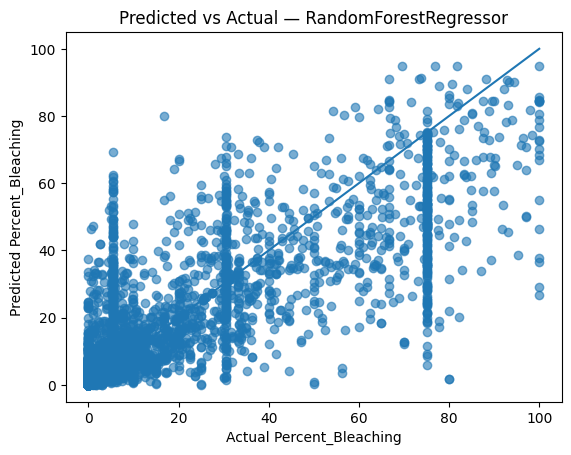
\includegraphics[width=0.75\textwidth]{rf.png}
    \caption{\textbf{Predicted vs.\ Actual Percent Coral Bleaching (Random Forest).}
    Each point represents one observation. The solid diagonal line indicates the ideal
    $y = x$ relationship where predicted bleaching equals observed bleaching.
    The upward trend shows the model captures overall bleaching patterns, though
    dispersion around the identity line reflects prediction error, particularly
    at extreme bleaching levels.}
    \label{fig:rf_pred_vs_actual}
\end{figure}

\subsection*{Exploratory Data Analysis}

Exploratory data analysis (EDA) was conducted in MATLAB to visualize trends, identify variability, and detect anomalies prior to modeling. \ref{fig:benthic-exploratory} and \ref{fig:wt-exploratory} illustrate pre-ARIMA patterns. EDA confirmed an inverse relationship between hard coral and algae cover, bleaching-related disruptions, and a long-term upward trend in sea surface temperatures, supporting the inclusion of seasonal components in the ARIMA model.

\begin{figure}[H]
    \begin{minipage}[t]{0.45\linewidth}
        \centering
        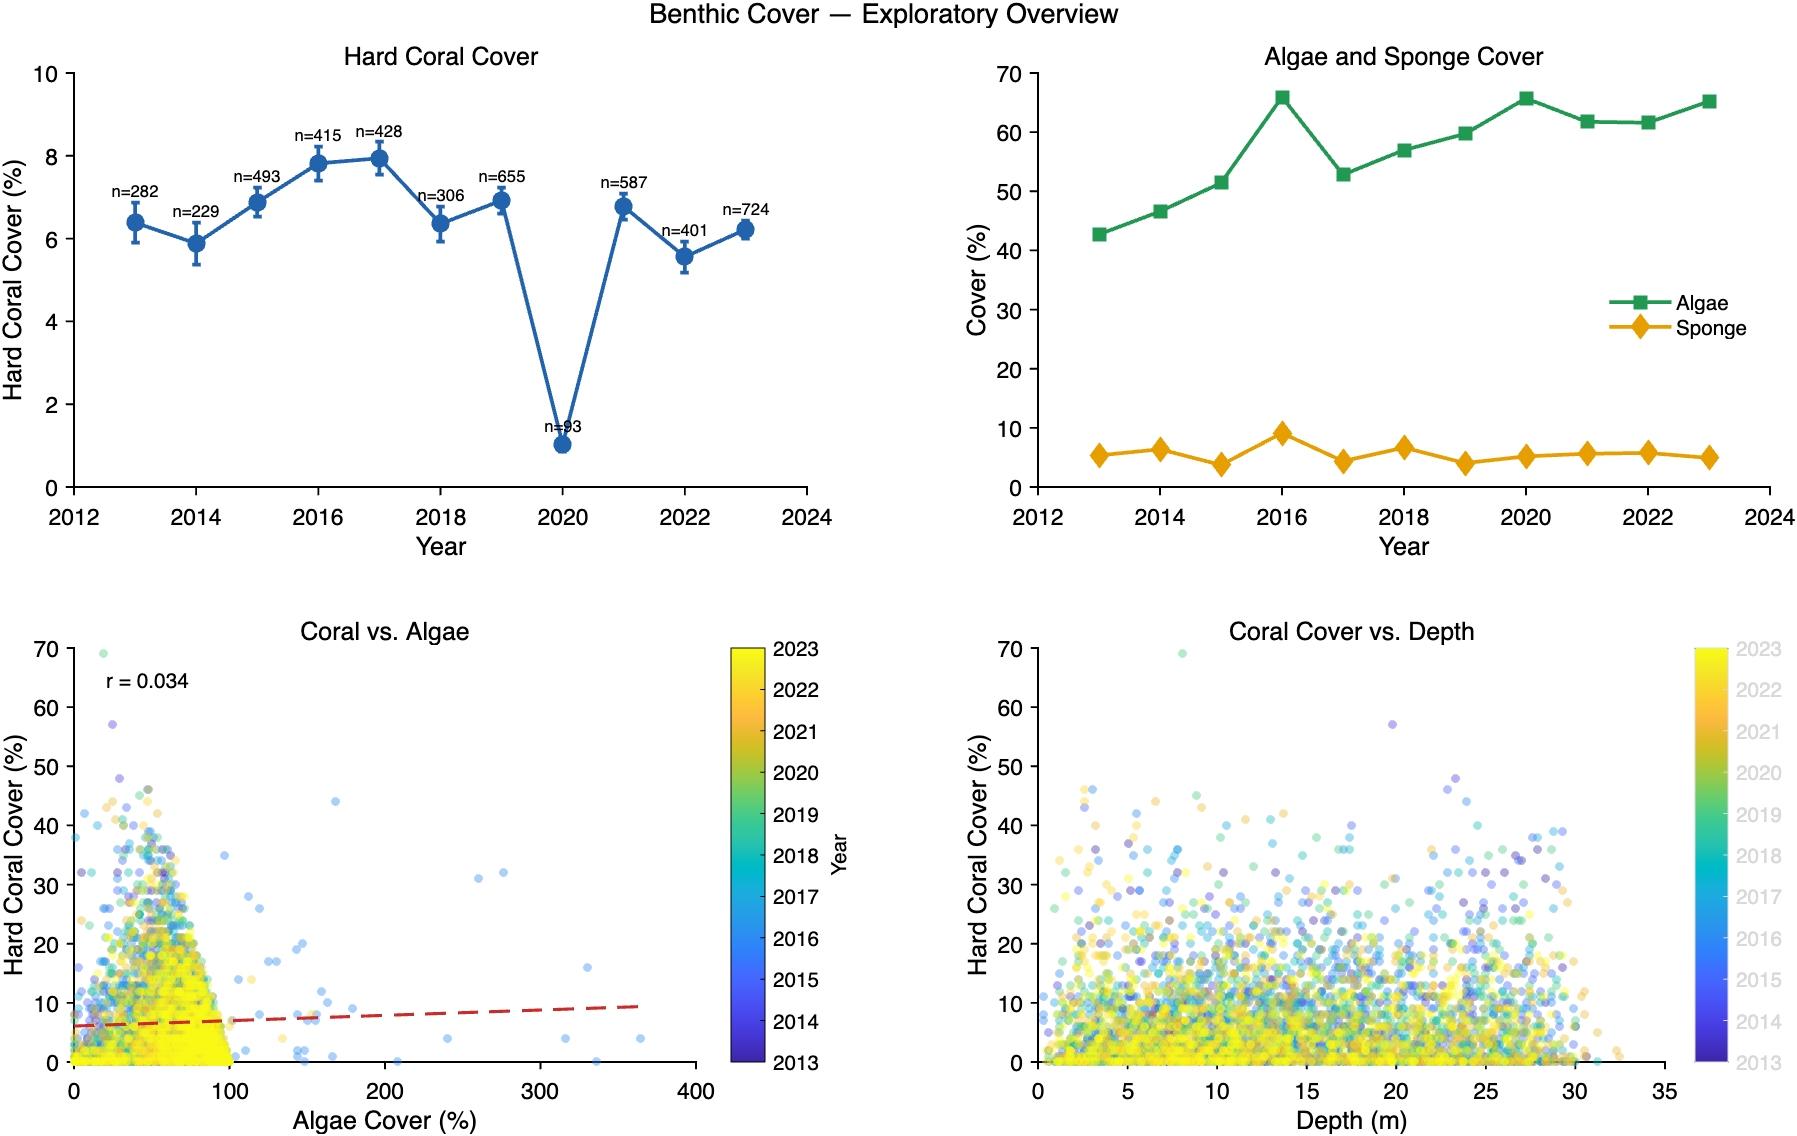
\includegraphics[width=\linewidth]{Figures/BenthicExploratory.png}
        \caption[Benthic cover pre-ARIMA]{Pre-ARIMA benthic cover visualization. Algae rises as coral cover declines, with hard coral near 6\%.}
        \label{fig:benthic-exploratory}
    \end{minipage}
    \hfill
    \begin{minipage}[t]{0.45\linewidth}
        \centering
        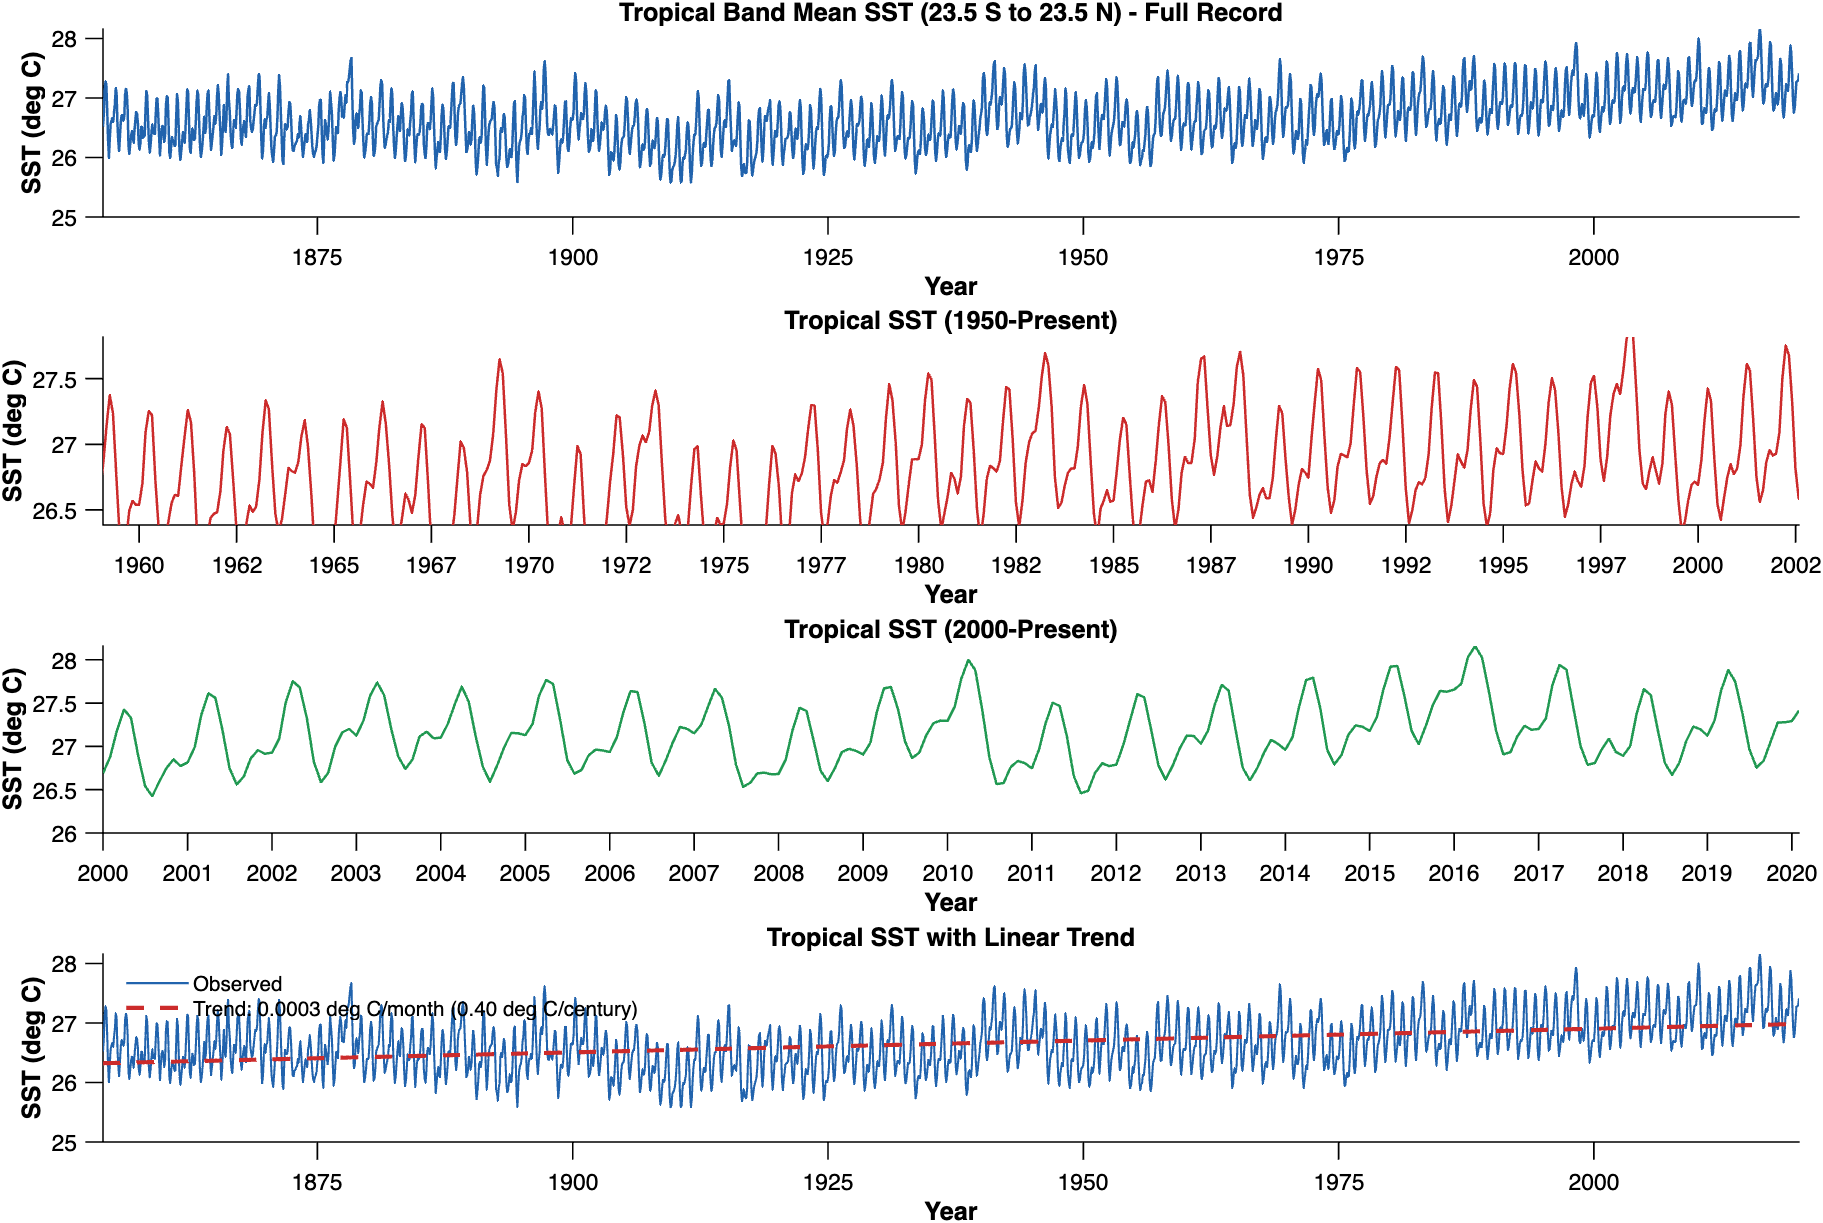
\includegraphics[width=\linewidth]{WTEXPLORE.png}
        \caption[Water temperature pre-ARIMA]{Pre-ARIMA water temperature visualization showing a steady SST increase in tropical regions.}
        \label{fig:wt-exploratory}
    \end{minipage}
\end{figure}

\subsection*{Machine Learning Regression Model for Coral Reef Bleaching}
This paper employed a supervised machine learning regression framework to predict coral bleaching severity as a continuous outcome variable using environmental predictors. Reef survey observations were compiled from NOAA Coral Reef Watch and related bleaching datasets \cite{noaa_crw}, including variables such as sea surface temperature (\texttt{SST}), Degree Heating Weeks (\texttt{DHW}), chlorophyll-$a$ concentration, turbidity, light availability, bathymetry, depth, and geographic coordinates. To extend the analysis beyond thermal stress alone, a carbonate chemistry dataset was incorporated, adding variables such as salinity, dissolved inorganic carbon, total alkalinity, pH, partial pressure of carbon dioxide (\texttt{pCO\textsubscript{2}}), and aragonite saturation state.

The carbonate chemistry observations were matched to bleaching survey points using spatial and temporal nearest-neighbor criteria. For each reef survey record, the closest carbonate observation in both location and time was identified, and match quality variables such as temporal offset and spatial distance were retained for analysis. Because carbonate chemistry data were not available for every bleaching observation, the final carbonate-enriched dataset consisted only of reef survey points with valid matched chemistry records. A baseline dataset containing only the original environmental predictors was also retained so that model performance could be compared before and after the addition of carbonate chemistry variables.

Several regression approaches were tested, including Random Forest Regression, Ridge Regression, and Linear Regression. These models were trained to predict percent coral bleaching from the environmental and carbonate chemistry predictors. The Random Forest model was especially well suited for this task because it can capture nonlinear relationships and higher-order interactions among structured tabular variables without requiring strong parametric assumptions.

Model performance was evaluated on a held-out test set using root mean squared error (\texttt{RMSE}), mean absolute error (\texttt{MAE}), and the coefficient of determination ($R^2$). To assess the contribution of carbonate chemistry, model performance on the carbonate-enriched dataset was compared against performance on the matched baseline dataset. Feature importance scores were extracted from the Random Forest model to support interpretation of predictor influence, and correlation analysis was conducted to examine direct associations between bleaching severity and the carbonate chemistry variables.

Together, the four models form a complete analytical pipeline: the ARIMA and SARIMAX models forecast the environmental trajectory, the Gordon-Schaefer and economic loss models translate that trajectory into fishery and financial losses, and the machine learning regression model estimates bleaching severity from environmental and carbonate chemistry conditions.


\subsubsection{Model Comparison and Carbonate Chemistry Integration}

To test whether carbonate chemistry improves bleaching prediction, baseline and carbonate-enriched models were compared on matched records only. After spatial-temporal matching, 1,463 of 14,592 observations were retained (10.03\%), so this analysis is conditional on the matched subset. Carbonate variables produced only small gains across models: Random Forest improved from \texttt{RMSE} 9.82 and $R^2=0.714$ to \texttt{RMSE} 9.76 and $R^2=0.717$; Ridge improved from 13.54/0.457 to 13.28/0.477; and Linear improved from 13.88/0.429 to 13.65/0.448. Random Forest remained the strongest model, and most predictive signal still came from heat stress, time, and location rather than carbonate chemistry.

\subsubsection{Breakpoint Analysis of Thermal Stress}

Piecewise regression identified a breakpoint at 8.01 Degree Heating Weeks (\texttt{DHW}) in the \texttt{SSTA\_DHW}-bleaching relationship. Bleaching rises quickly below this threshold, shifts sharply near 8 \texttt{DHW} (onset of severe bleaching), and then increases more slowly, consistent with partial saturation among already affected corals. This threshold aligns with NOAA Coral Reef Watch guidance \cite{noaa_crw}, supporting a nonlinear, threshold-driven bleaching response dominated by cumulative thermal stress.

\subsubsection{Feature Importance in the Random Forest Regressor}

Feature-importance results from the carbonate-enriched Random Forest show that bleaching severity is driven mainly by temporal, thermal, and spatial structure. \texttt{Year} was the top predictor (36.3\%), followed by \texttt{TSA\_DHW} (12.4\%), while longitude and latitude were also strong contributors. Match-quality features (temporal offset and spatial distance) had moderate influence, indicating pairing precision matters. Carbonate variables (salinity, DIC, alkalinity, pH, $p\mathrm{CO}_2$, aragonite saturation) contributed comparatively little, so they act as secondary predictors in this model.

\subsubsection{Correlation Patterns in Carbonate Chemistry Variables}

Correlation analysis found weak direct linear relationships between bleaching severity and matched carbonate variables; salinity, aragonite saturation state, $p\mathrm{CO}_2$, and carbonate-derived temperature were all near zero correlation. This is consistent with model-comparison and feature-importance results: carbonate chemistry adds limited incremental signal in the current dataset and likely acts through nonlinear or context-dependent pathways. Overall, bleaching severity is explained primarily by cumulative heat stress, temporal escalation, and spatial variation. Together with Gordon-Schaefer fishery losses and the coastal-tourism economic model, these results provide the baseline for the intervention sensitivity analysis below.

\begingroup
\setstretch{1.1}
\renewcommand{\arraystretch}{1.1}
\rowcolors{2}{gray!15}{white}
\begin{xltabular}{\textwidth}{>{\centering\arraybackslash}p{1.0cm}
                               >{\centering\arraybackslash}p{3.6cm}
                               >{\centering\arraybackslash}p{2.8cm}
                               >{\centering\arraybackslash}p{2.8cm}
                               >{\centering\arraybackslash}X}
\rowcolor{white}\caption{SARMA and SARIMAX Hard Coral Cover Forecasts from 2024--2049}
\label{tab:arima-forecast}\\
\toprule
\rowcolor{white}\textbf{Year} & \textbf{SARMA Forecast} & \textbf{Lower 95\%} & \textbf{Upper 95\%} & \textbf{SARIMAX Forecast} \\
\midrule
\endfirsthead
\rowcolor{white}\multicolumn{5}{c}{\tablename\ \thetable{} -- \textit{continued from previous page}} \\[4pt]
\toprule
\rowcolor{white}\textbf{Year} & \textbf{SARMA Forecast} & \textbf{Lower 95\%} & \textbf{Upper 95\%} & \textbf{SARIMAX Forecast} \\
\midrule
\endhead
\midrule
\rowcolor{white}\multicolumn{5}{r}{\textit{Continued on next page}} \\
\endfoot
\bottomrule
\endlastfoot
2024 & 5.32 & 3.67 & 6.97 & 9.32 \\
2025 & 6.18 & 3.41 & 8.96 & 5.51 \\
2026 & 5.58 & 2.69 & 8.47 & 5.13 \\
2027 & 4.74 & 1.84 & 7.64 & 5.34 \\
2028 & 2.97 & 0.07 & 5.88 & 0.91 \\
2029 & 3.95 & 1.04 & 6.85 & 5.30 \\
2030 & 3.48 & 0.58 & 6.38 & 4.77 \\
2032 & 5.62 & 2.72 & 8.52 & 8.61 \\
2036 & 1.79 & 0.00 & 4.69 & 0.07 \\
2040 & 4.36 & 1.45 & 7.26 & 7.72 \\
2044 & 0.58 & 0.00 & 3.49 & 0.00 \\
2048 & 3.09 & 0.19 & 6.00 & 6.78 \\
2049 & 1.89 & 0.00 & 4.80 & 2.41 \\
\end{xltabular}
\endgroup


\textbf{NOTE TO ATHARV: BRO JUST MAKE THE INTERVALS LARGER HERE MAKE IT LIKE 20 YEARS EACH BUMP SINCE YOU'LL RUN UNTIL 2100}


\subsection*{GitHub Repository}
The full data processing scripts, model code, and generated figures are archived in the project GitHub repository. The top-level structure follows a standard workflow layout: \texttt{data/} contains raw and cleaned datasets by region, \texttt{notebooks/} contains the code used to clean the data, \texttt{outputs/} contains exported plots used in this report, and \texttt{MATLAB/} contains the code used to simulate the models. The repository can be found at
\url{https://github.com/coreylu2027/CAAARal-Reefs/tree/main}.

\newpage

\newpage
\addcontentsline{toc}{section}{References}
\begingroup
\setstretch{1.0}
\bibliographystyle{plainnat}
\bibliography{refs}
\endgroup

\end{document}